\documentclass[degree=bachelor]{thuthesis}
% 选项:
%   type=[bachelor|master|doctor|postdoctor], % 必选
%   secret,                                   % 可选
%   pifootnote,                               % 可选(建议打开)
%   openany|openright,                        % 可选,基本不用
%   arial,                                    % 可选,基本不用
%   arialtoc,                                 % 可选,基本不用
%   arialtitle                                % 可选,基本不用

% 所有其它可能用到的包都统一放到这里了,可以根据自己的实际添加或者删除。
\usepackage{thuthesis}
\newcommand{\transpose}[1]{\ensuremath{#1^{\scriptscriptstyle T}}}
\DeclareMathOperator*{\rgmax}{argmax}
\DeclareMathOperator*{\rgmin}{argmin}
\DeclareMathOperator{\Tr}{Tr}
% 定义所有的图片文件在 figures 子目录下
\graphicspath{{figures/}}

% 可以在这里修改配置文件中的定义。导言区可以使用中文。

\begin{document}

%%% 封面部分
\frontmatter
\thusetup{
  %******************************
  % 注意:
  %   1. 配置里面不要出现空行
  %   2. 不需要的配置信息可以删除
  %******************************
  %
  %=====
  % 秘级
  %=====
  secretlevel={秘密},
  secretyear={10},
  %
  %=========
  % 中文信息
  %=========
  ctitle={无线网络中定位信息的时空传播机理研究},
  cdegree={理学学士},
  cdepartment={数学科学系},
  cmajor={数学与应用数学},
  cauthor={赵丰},
  csupervisor={沈渊\quad 副教授},
  %cassosupervisor={梁恒\quad 副教授}, % 副指导老师
  ccosupervisor={梁恒\quad 副教授}, % 联合指导老师
  % 日期自动使用当前时间,若需指定按如下方式修改:
  % cdate={超新星纪元},
  %
  % 博士后专有部分
  cfirstdiscipline={计算机科学与技术},
  cseconddiscipline={系统结构},
  postdoctordate={2009年7月——2011年7月},
  id={编号}, % 可以留空: id={},
  udc={UDC}, % 可以留空
  catalognumber={分类号}, % 可以留空
  %
  %=========
  % 英文信息
  %=========
  etitle={An Introduction to \LaTeX{} Thesis Template of Tsinghua University v\version},
  % 这块比较复杂,需要分情况讨论:
  % 1. 学术型硕士
  %    edegree:必须为Master of Arts或Master of Science(注意大小写)
  %             “哲学、文学、历史学、法学、教育学、艺术学门类,公共管理学科
  %              填写Master of Arts,其它填写Master of Science”
  %    emajor:“获得一级学科授权的学科填写一级学科名称,其它填写二级学科名称”
  % 2. 专业型硕士
  %    edegree:“填写专业学位英文名称全称”
  %    emajor:“工程硕士填写工程领域,其它专业学位不填写此项”
  % 3. 学术型博士
  %    edegree:Doctor of Philosophy(注意大小写)
  %    emajor:“获得一级学科授权的学科填写一级学科名称,其它填写二级学科名称”
  % 4. 专业型博士
  %    edegree:“填写专业学位英文名称全称”
  %    emajor:不填写此项
  edegree={Doctor of Engineering},
  emajor={Computer Science and Technology},
  eauthor={Xue Ruini},
  esupervisor={Professor Zheng Weimin},
  eassosupervisor={Chen Wenguang},
  % 日期自动生成,若需指定按如下方式修改:
  % edate={December, 2005}
  %
  % 关键词用“英文逗号”分割
  ckeywords={协作定位,费舍尔信息矩阵,定位误差下界,矩阵代数,连分式},
  ekeywords={Cooperative localization, Fisher informaton matrix, Position error bound, Matrix algebra, Continued fraction}
}

% 定义中英文摘要和关键字
\begin{cabstract}
对于目标实时位置的获取是无线通信技术应用的重要组成部分。在多个目标节点的定位场景下,基于目标节点相互之间的距离信息的协作定位技术能够有效提高定位精度。但是协作定位网络也不可避免的存在定位误差,如何根据网络中的拓扑特点和几何参数尽可能降低定位误差是这一领域热门的研究课题。特别的,随着定位网络规模的扩大和时间上的延长,各种测量数据如何影响定位误差是本文研究的内容。

  本文从高斯信号模型出发,从费舍尔信息矩阵的角度刻画了定位误差的时空衰减特性。本文主要运用了矩阵代数的运算规则推导了费舍尔信息矩阵特征值的闭式表达式,并利用函数的连分式展开的分析方法求出了定位误差的时空衰减速度的量阶,从而揭示了定位误差与协作信息的关系的一般机理。

  本文在单节点时间协作问题上得出了一般情形下误差下界的连分式表达形式,并且在理论上证明了采样时间间隔趋于零时的误差下界和节点的运动轨迹无关的性质,这对于单节点路径规划与运动控制有一定的理论指导意义。
\end{cabstract}

% 如果习惯关键字跟在摘要文字后面,可以用直接命令来设置,如下:
% \ckeywords{协作定位,费舍尔信息矩阵, 定位误差下界,矩阵代数,连分式}

\begin{eabstract}
The acquisition of real-time target position is an important part of application in wireless communication technology. For situations where positions of multiple agents are required, cooperative localization technology based on distance measure information between agents can significantly improve the localization accuracy. However, localization error is unavoidable in cooperative localization network and it is a vital topic in this field to investigate how to decrease localization error based on topological characteristics and geometrical parameter. In particular, it is the main focus of this article to make research on how the localization error is affected by distance measure information, as the scale of the network is growing and observation time is prolonging.

Starting from Gaussian signal model, this article discussed the spatial-temporal decaying characteristics of localization error from the perspective of Fisher information matrix. Applying rules of matrix algebra, the closed form of eigenvalues for special Fisher information matrix is derived; With the method of continued fraction analysis, the decaying order of localization error propagation speed is derived, which shows the general mechanism of the relationship between localization error and cooperative information.

In this article, general form of error bound is derived in continued fraction form for single agent temporal cooperation case, and we proved that the error bound is unrelated with trajectory of the agent as the sampling time interval tends to zero. This result could show some insights in the domain of trajectory planning and motion control of network agent.

\end{eabstract}

% \ekeywords{\TeX, \LaTeX, CJK, template, thesis}

% 如果使用授权说明扫描页,将可选参数中指定为扫描得到的 PDF 文件名,例如:
\makecover

%% 目录
\tableofcontents

%% 符号对照表
\begin{denotation}[3cm]
\item[$N_b$] 锚点数量
\item[$\bm{p}_i$] 第i个待定位节点的位置,在时间协作中表示目标节点各个时刻的位置
\item[$\bm{P}$] 全部要估计的待定位节点的位置向量,即$(\bm{p}_1,\bm{p}_2,\dots,\bm{p}_{N_a})$
\item[$\bm{p}^b_i$] 第i个锚点的位置
\item[$f(x_1,\dots,x_n|\theta)$] 参数$\theta$已知条件下随机变量$X_1,\dots,X_n$联合概率密度函数
\item[$\bm{I}(\bm{p})$] 关于待定位节点位置$\bm{p}$的费舍尔信息矩阵
\item[$N_a$] 待定位节点数量,在时间协作中表示采样的数量
\item[$\sigma^2_{i}$] 待定位节点和锚点i之间测距的方差
\item[$\sigma^2_{i,j}$] 节点i和节点j之间测距的方差
\item[$\bm{u}_{i,j}$] 节点i和节点j之间的单位方向向量,时间协作中表示采样时刻$t_i$和$t_j$之间目标节点的位置变化向量
\item[$\bm{C}_{i,j}$] 费舍尔信息矩阵位于i行j列的元素的相反数
\item[$\Delta t$] 时间协作中采样时间间隔
\item[$\lambda_{i}$] $\sigma^2_{i}$的倒数
\item[$\bm{u}_i$] 待定位节点和锚点i之间的单位方向向量,时间协作中表示第i个时刻的位置和第i+1个时刻的位置之间的单位方向向量
\item[$\phi_i$] $\bm{u}_i$的方向角,时间协作中表示第$t_i$时刻$\bm{u}_{i,i+1}$的方向角
\item[$\bm{A}^{-1}_{1\times2,1\times2}$] 方阵$\bm{A}$的逆阵由前两行和前两列决定的子矩阵
\end{denotation}



%%% 正文部分
\mainmatter
\chapter{引言}
\label{cha:intro}

\section{研究背景}
%background info here
对于目标的实时位置的获取是无线通信技术的应用的重要一部分\cite{indoorPos},其在仓库管理、车辆导航与编队、军事演习等方面有着广泛的应用前景。


%tech info here
通常一个无线定位系统可以依赖于GPS卫星定位,但在室内定位的场合,由于微波被建筑物散射等原因,定位效果并不理想。在这种情况下需要根据应用的场景开发
地面无线定位系统。通常一个地面无线定位系统会事先部署一些位置已知的锚点(基站),并采用某个特殊的频段的电磁波如超宽带(Ultra Wideband)与位置未知的目标节点进行通信。在锚点处可以通过测量无线信号到达的时间或信号强度等信息估计出某个基站与场景中目标节点的距离,
%如果是对目标的追踪的情形可以利用两个时刻间速度的测量结果得到距离信息,
利用统计学的方法对这些数据进行实时的处理,可以估计出目标节点的位置或运动的轨迹。


%non-cooperative case to cooperative case
传统的定位方法是只利用锚点和目标节点彼此之间的测距信息对目标节点进行定位,在一些环境比较苛刻的定位场景,要达到较高的定位精度锚点部署的密度和功耗都要比较大,因而需要的成本也随之提高。在有多个目标节点的定位场景下,随着技术的成熟近年来发展出了利用目标节点之间相互通信得到的距离信息的协作定位技术,协作定位技术不仅利用了目标节点和已知位置的锚点之间的信息,还利用了目标节点彼此之间的定位信息,不仅可以提高定位精度,也降低了开销。
已知协作网络中的测量信息后,网络中各个节点在上一轮的位置信息可以用来校准它的邻居节点的位置以提高定位精度,多轮的协作使网络中的节点可以和超出其通信范围的其他较远的节点间接地协作,并最终达到稳态,这是静态协作网络的典型场景。
在对节点的位置有实时性要求的场合,网络中各个节点还可以利用自身之前时刻位置的估计值来对自身当前时刻进行定位,这方面比较著名的算法有卡尔曼滤波\cite{KF}等方法。

%algorithm property analysis
协作定位技术已经有了一定的研究基础,目前已经有大量的文献针对定位算法展开探讨,对定位算法的性能分析需要对定位误差能够量化,定位误差最常采用的方法是使用估计量的均方误差来量化。如果估计量是无偏的,可以知道估计量的均方误差总是在克拉美罗界之上\cite{siyi}。克拉美罗界是根据估计量的费舍尔信息量计算出来的均方误差的理论下界,因此费舍尔信息量可以作为衡量定位精度的理论上界。在本文中我们将主要从费舍尔信息量的角度研究定位误差。

从原始信号中可以提取的观测数据的有多种,一般常用的有信号到达时间(time-of-arrival),信号到度角度(angle-of-arrival),以及接收信号强度(received-signal-strength)等。基于这些不同的观测数据建立的模型有一定区别,由此导出的定位误差下界也不相同。文献\cite{LimitBound}针对不同的观测量研究了定位误差下界的规律,在本文的研究中主要针对信号到达时间这一观测,因为由信号到达时间乘以光速即可得到距离的测量量,所以本文在数学模型第\ref{cha:model}章中直接假设距离是观测量。

实际定位系统中无线信号受环境条件的限制,传播过程中会出现非视距(non-light-of-sight)和多径(multi-path)等问题\cite{indoorPos},这给定位误差的分析增加了难度,为了反映实际,通常在数学模型中会把由非视距和多径效应带来的额外信道参数作为未知的估计量与节点的位置估计量一并考虑\cite{LimitBound}。另一个性能瓶颈是不同节点之间彼此的数字时钟不一定完全同步(clock synchronization)而引入的测距误差\cite{indoorPos},时钟同步问题一方面可以通过系统设计尽量减轻其带来的影响,另一方面也可以用统计的方法将时钟偏移作为未知参数,在数据处理阶段进行处理来降低时钟不同步带来的定位误差。本文中的模型为能够研究问题的机理而建立的模型比较简单,并不考虑这些信道参数带来的影响。

对定位误差理论下界的研究工作不仅可以为不同的定位算法提供可以参照的最优定位结果,也可以指导定位网络中节点的部署。在研究方法方面可以采用理论推导和仿真比较相结合的方法:在理论推导方面,文献\cite{LimitBound}探讨了多径和非视距传播对定位误差下界的影响,并推导了定位误差下界的上下界;对于定位误差界随链路衰减的特征在文献\cite{siyi}中已经有了一些比较宏观的刻画。在文献\cite{LimitBound},\cite{siyi}的研究工作基础上,本文进一步分析这个定位误差下界随着定位网络规模的扩大和采样时间间隔的缩短的规律,探究协作定理网络的信息耦合机理。

%research of others in synthesis
%  在文献\cite{LimitBound2}中为研究定位误差下界提出了等效费舍尔信息矩阵、信息椭圆等概念,同时对两个节点协作的简单场景分析了定位误差和定位%信息强度的关系;本文中会引用\cite{LimitBound2}中相关的结论,同时在必要之处会采用新的数学方法给出更加简洁的结论推导。
\section{研究问题}
%content
%research current state here
在本人的研究中,会首先建立定位网络的数学模型并根据建立的模型推导定位误差下界的一般表达式,然后分别针对若干特殊的定位网络推导误差下界的解析表达式,并根据解析表达式辅助以必要的数值计算分析定位性能随网络的时空规模的变化规律。

%focus
\section{文章结构}
本文的研究重点是特殊定位网络误差下界的推导,在第(\ref{cha:model})章中给出了问题的数学模型,主要分非协作定位场景(\ref{section:noncooperative_localization})、空间协作定位场景(\ref{section:cooperative_localization})、时间协作定位场景(\ref{section:temporal_cooperative_localization})三部分,(\ref{section:model_discussion})一节中对模型的合理性进行了进一步讨论。
在第(\ref{cha:content3})章中分别对上一节提出的数学模型进行初步的分析和求解,其中非协作情形(\ref{section:circle_general})针对小节(\ref{section:noncooperative_localization})的模型,空间两个节点协作(\ref{section:two_node_cooperation})
针对(\ref{section:cooperative_localization})的模型。
在第(\ref{cha:content4})章中分别对上一节提出的数学模型进行深入的分析和求解,其中N个节点两两协作(\ref{section:complete_graph_cooperation})、大规模正方形和正六边形网络协作(\ref{section:square_and_hexagon_network})
针对(\ref{section:cooperative_localization})的模型,一个节点时间上的协作(\ref{section:linear_network})针对(\ref{section:temporal_cooperative_localization})的模型。
最后第(\ref{cha:content5})章对全文使用的数学方法和取得的成果进行了总结。
\chapter{数学模型}\label{cha:model}
\section[非协作定位场景]{非协作定位场景}\label{section:noncooperative_localization}

        考虑一个平面定位场景中部署了$N_b$个位置已知的\textbf{锚点},锚点的位置记为$\{\bm{p}^b_1,\bm{p}^b_2,...\bm{p}^b_{N_b}\}$,现在要对场景中一个\textbf{位置未知}的节点进行定位,待定位节点的位置为$\bm{p}$,如图(\ref{fig:non_cooperative_spatial})所示。
        \begin{figure}
          \centering
        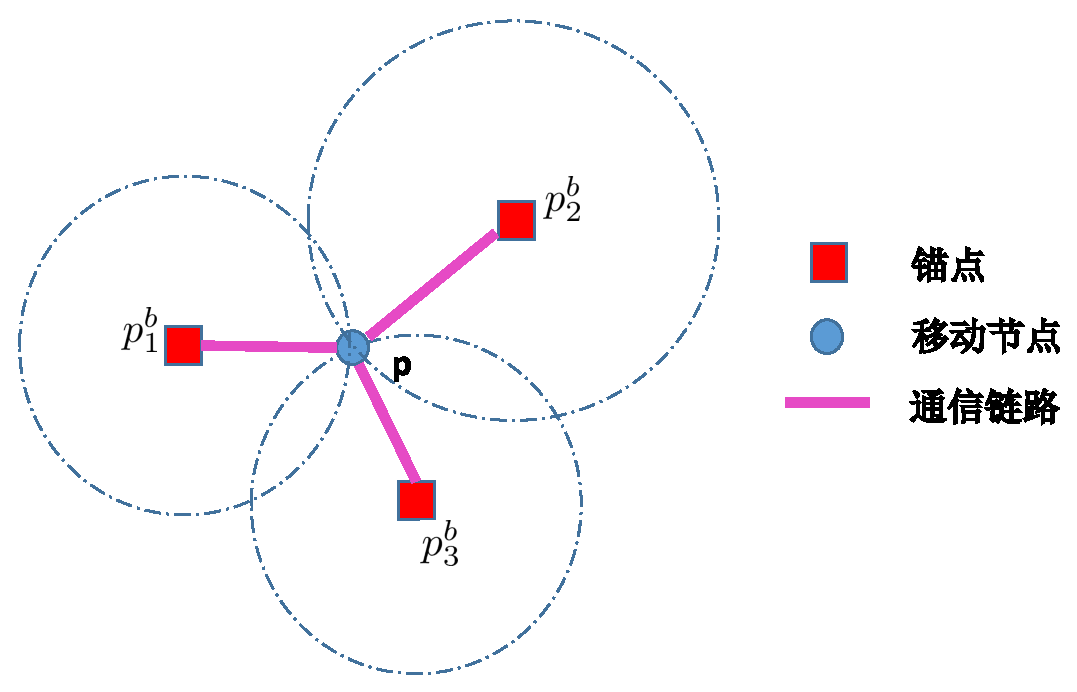
\includegraphics[width=300pt]{non_cooperative_spatial.eps}
          \caption{非协作静态场景下的定位}\label{fig:non_cooperative_spatial}
        \end{figure}
假设\textbf{待定位节点}和每一个锚点都可以相互通信进行无线测距,距离测量量服从均值为$||\bm{p}^b_i-\bm{p}||$,方差为$\sigma_i$的正态分布$X_i$。

$N_b$个\textbf{独立}测量量的联合概率分布为:
\begin{equation}\label{eq:single}
f(x_1,...x_{N_b}|\textbf{p})=\prod_{i=1}^{N_b}\frac{1}{\sqrt{2\pi\sigma_i^2}}exp\left(-\frac{(x_i-||\bm{p}^b_i-\bm{p}||)^2}{2\sigma_i^2}\right).
\end{equation}

根据点估计的理论,对于一个无偏估计量,它的方差的下界是\textbf{费舍尔信息量}(Fisher Information)的倒数,称之为\textbf{克拉美罗界}(Crame Rao Bound),在本文的讨论中,也称之为定位误差下界(Spatial Position Error Bound),它的计算公式为:
\begin{equation}\label{eq:SPEB_formula}
  \text{SPEB}=\text{tr}(\bm{I(\bm{p})}^{-1}).
\end{equation}
  % - A title should summarize the slide in an understandable fashion
  %   for anyone how does not follow everything on the slide itself.


{费舍尔信息矩阵}
以节点的\textbf{2维}位置为待估计参数,费舍尔信息量推广为\textbf{费舍尔信息矩阵}(Fisher Information Matrix)。

对于我们的模型问题,费舍尔信息矩阵有如下的形式:
\begin{equation}\label{eq:uu}
I(\bm{p})=\displaystyle\sum_{i=1}^{N_b}\frac{1}{\sigma_i^2}\bm{u}_i\bm{u}_i^{\textrm{T}}
\end{equation}
其中
\begin{equation}
\bm{u_i}=\frac{\bm{p}^b_i-\bm{p}}{||\bm{p}^b_i-\bm{p}||}.
\end{equation}


\section[协作定位场景]{协作定位场景}\label{section:cooperative_localization}

考虑一个平面定位场景中不仅部署了$N_b$个位置已知的锚点,还有$N_a$个位置未知的待定位节点,某些位置未知的节点之间可以\textbf{彼此测距},如图(\ref{fig:cooperative_spatial})所示。第i和第j个未知节点距离测量量服从均值为$||\bm{p}_i-\bm{p}_j||)$,方差为$\sigma_{ij}$的正态分布$X_{ij}$。
        \begin{figure}
          \centering
          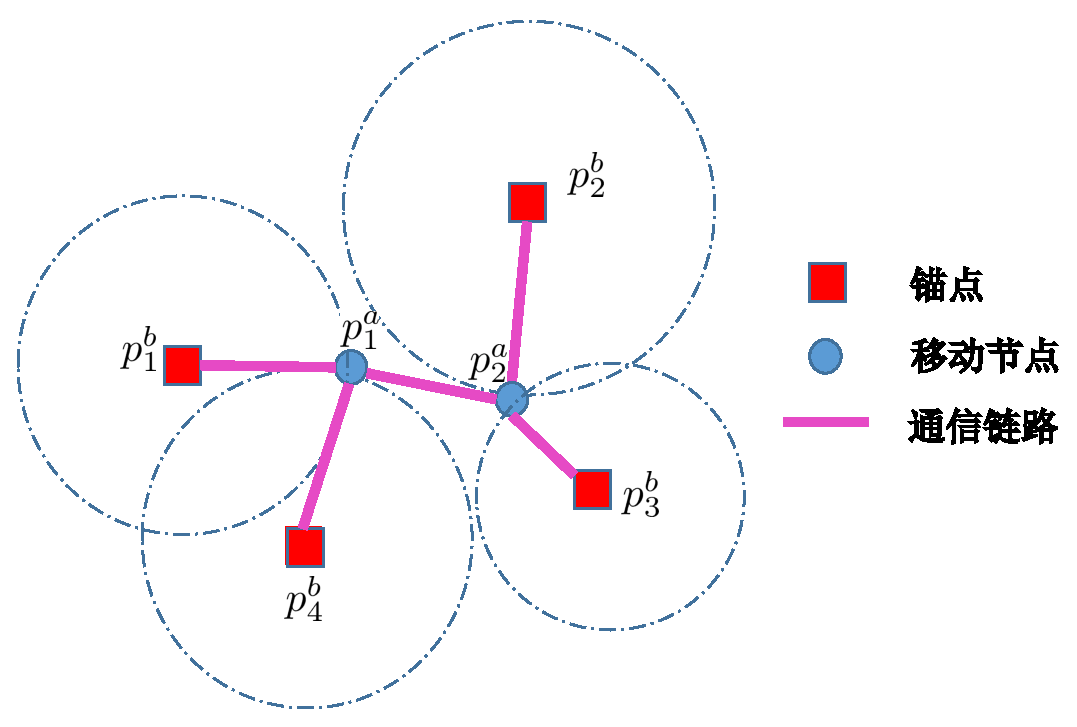
\includegraphics[width=300pt]{cooperative_spatial.eps}
          \caption{协作静态场景下的定位}\label{fig:cooperative_spatial}
        \end{figure}

以$N_a$个未知节点的位置$\{p_i\}$作为待估计的参数,可以得到测距量的联合概率密度函数为

\begin{equation}
F(\bm{X}|\bm{P})=\prod_{i=1}^{N_a} f(x^i_1,...x^{i}_{N_b}|\bm{p_i})\prod_{(i,j)\in \mathcal{E}}\frac{1}{\sqrt{2\pi\sigma_{ij}^2}}exp\left(-\frac{(x_{ij}-||\bm{p}_i-\bm{p}_j||)^2}{2\sigma_{ij}^2}\right).
\end{equation}
上式中f的具体表达式为式(\ref{eq:single}),$\mathcal{E}$表示可以彼此测距的未知节点的二元组的集合,而$x_t^i$表示第t个锚点和第i个未知节点的距离测量量。


仿照单节点时费舍尔信息矩阵的推导,关于$2N_a$个参数$\{p_i\}$的费舍尔信息矩阵$\bm{I}(\bm{P})$有如下的表达形式:
\begin{equation}\label{eq:general_fim}
\bm{I}(\bm{P})=
\left(
\begin{array}{cccc}
I(\bm{p}_1)+&-\bm{C}_{1,2}&...&-\bm{C}_{1,N_a}\\
\sum_{j\in \{1,..N_a\}\backslash\{1\}}\bm{C}_{1,j}&&&\\
&&&\\
-\bm{C}_{1,2} & I(\bm{p}_2)+
&...&-\bm{C}_{2,N_a}\\
&\sum_{j\in \{1,..N_a\}\backslash \{2\}}\bm{C}_{2,j}&&\\
&&&\\
\vdots &\vdots&\ddots &\vdots\\
&&&\\
&&&I(\bm{p}_{N_a})+\\
-\bm{C}_{1,N_a}&-\bm{C}_{2,N_a}&...& \sum_{j\in \{1,..N_a\}\backslash\{N_a\}}\bm{C}_{N_a,j}\\
\end{array}
\right).
\end{equation}
上面的式子中$I(\bm{p}_i)$表示$N_b$个锚点对未知节点距离测量的贡献,和前面的(\ref{eq:uu})式相同。$C_{i,j}=\bm{1}_{(i,j)\in E}\bm{u}_{ij}\bm{u}_{ij}^{\textrm{T}} /\sigma^2_{ij}$,表示未知节点i和j协作的矩阵。
$\bm{u}_{ij}=\frac{\bm{p}_i-\bm{p}_j}{||\bm{p}_i-\bm{p}_j||}$表示未知节点i和j的方向向量。
\section[时间协作定位]{时间协作定位}\label{section:temporal_cooperative_localization}

\subsection{单个待测节点时间协作定位}

考虑一个平面定位场景中有一个待定位的移动节点,场景中部署的$N_b$个位置已知的锚点分别在在$t_1,\dots,t_{N_a}$时刻对该节点进行定位,移动节点可以通过自身的加速度传感器对自己的速度有测量,如图(\ref{fig:cooperative_single_temporal})所示。
        \begin{figure}
          \centering
          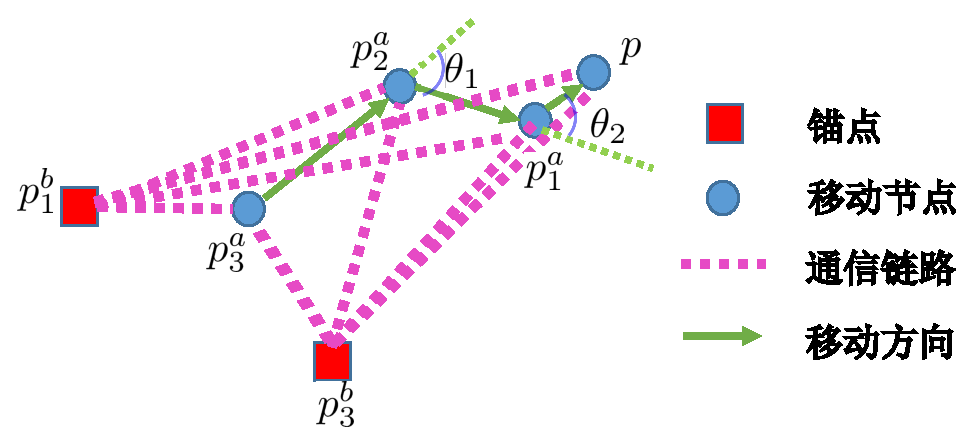
\includegraphics[width=300pt]{cooperative_single_temporal.eps}
          \caption{协作动态场景下的定位}\label{fig:cooperative_single_temporal}
        \end{figure}

假设测量时间间隔比较小使得相邻测量间节点速度方向可近似看作不变,速度测量值服从均值为$v$,方差为$\sigma_{v}$的正态分布$V_{ij}$。
那么以节点各时刻的的位置$\{p_i\}$作为待估计的参数,可以得到包括相邻时刻间的所有测距量的联合概率密度函数为
\begin{equation}
F(\bm{X}|\bm{P})=\prod_{i=1}^{N_a} f(x^i_1,...x^{i}_{N_b}|\bm{p_i})
\prod_{i=1}^{N_a-1}\frac{1}{\sqrt{2\pi}\sigma_v(t_{i+1}-t_i)}
exp\left(-\frac{(v_{i,i+1}(t_{i+1}-t_i)-||\bm{p}_i-\bm{p}_{i+1}||)^2}{2\sigma_v^2(t_{i+1}-t_i)^2}\right).
\end{equation}
费舍尔信息矩阵关于$2N_a$个参数$\{p_i\}$的费舍尔信息矩阵有如下的表达形式:
\begin{equation}\label{eq:time_cooperation_matrix}
\bm{I}(\bm{P})=
\left(
\begin{array}{ccccc}
I(\bm{p}_1)+\bm{C}_{1,2}&-\bm{C}_{1,2}&\bm{0}&\dots&\bm{0}\\
&&&&\\
-\bm{C}_{1,2} & I(\bm{p}_2)+\bm{C}_{1,2}+\bm{C}_{2,3}&-\bm{C}_{2,3}&\dots&\bm{0}\\
\vdots &\vdots&\ddots &\vdots&\vdots\\
&&&&\\
\bm{0}&\bm{0}&...& -\bm{C}_{N_a-1,N_a}&\bm{C}_{N_a-1,N_a}+I(\bm{p}_{N_a})\\
\end{array}
\right).
\end{equation}
上面的式子中若将2乘2的矩阵看作单位元素,则是一个三对角的矩阵。$I(\bm{p}_i)$表示$N_b$个锚点对未知节点距离测量的贡献,和前面的(\ref{eq:uu})式相同。$C_{i,i+1}=\bm{1}_{(i,j)\in E}\bm{u}_{ij}\bm{u}_{ij}^{\textrm{T}} /(\sigma_v^2(t_{i+1}-t_i)^2)$,表示未知节点i和j协作的矩阵,$\bm{u}_{ij}$表示未知节点i和j的方向向量。

\subsection{两个待测节点时间上一次协作}

考虑一个平面定位场景中有两个待定位的移动节点$p,q$,在初始时刻$t_1$两个移动节点之间有一次测距,服从无偏的标准差为$\sigma$的正态分布,之后时刻$t_2,\dots,t_{N_a}$两个节点不再协作,在各个时刻场景中部署的$N_b$个位置已知的锚点都可以对两个节点进行定位,移动节点可以通过自身的加速度传感器对自己的速度有测量,
假设时间间隔比较小使得相邻测量间节点速度方向可近似看作不变,速度测量值分别服从方差为$\sigma_i$的正态分布$V_i$和标准差为$\sigma'_i$的正态分布$V'_i$(均值未知,但测量是无偏的),同时假设每个节点从$t_i$到$t_{i+1}$时刻的角度符从$[0,2\pi]$的正态分布,但角度没有测量量,是未知参数。我们试图研究初始时刻$t_1$两个移动节点之间的一次测距对后续$t_n$时刻每个节点的定位精度平均来说还有多大的贡献?

针对两个节点各时刻的的位置$\{p_i,q_i\}$共计$2N_a$个二维向量作为待估计的参数,可以得到包括相邻时刻间的所有测距量的联合概率密度函数为
\begin{equation}
\begin{split}
F(\bm{X}|\bm{P})&=\frac{1}{\sqrt{2\pi\sigma^2}}exp\left(-\frac{(x-||\bm{p}_1-\bm{q}_1)^2}{2\sigma^2}\right)\prod_{i=1}^{N_a}
f(x^i_1,...x^{i}_{N_b}|\bm{p_i})
\prod_{i=1}^{N_a} f(x^i_1,...x^{i}_{N_b}|\bm{q_i})\\
&\prod_{i=1}^{N_a-1}\frac{1}{\sqrt{2\pi}\sigma_i(t_{i+1}-t_i)}
exp\left(-\frac{(v_i(t_{i+1}-t_i)-||\bm{p}_i-\bm{p}_{i+1}||)^2}{2\sigma_i^2(t_{i+1}-t_i)^2}\right)\\
&\prod_{i=1}^{N_a-1}\frac{1}{\sqrt{2\pi}\sigma'_i(t_{i+1}-t_i)}
exp\left(-\frac{(v'_i(t_{i+1}-t_i)-||\bm{q}_i-\bm{q}_{i+1}||)^2}{2\sigma^{'2}_i(t_{i+1}-t_i)^2}\right).
\end{split}
\end{equation}
我们可以将第二个模型问题与线性网络单节点时间协作建立联系,只需对上面概率密度函数中出现的符号重排即可:
将两移动节点在$t_1$时刻的协作的边作为链路的中心,该链路记为$l$,左右各有$N_a$个节点,分别表示各节点$t_i$时刻的位置。
以其中一个移动节点为参照,研究其$t_{N_a}$时刻的位置在有无$l$的影响,无$l$时,协作链路长度只有$N_a-1$,有$l$时,协作链路长度是$2N_a-1$,增加了$N_a$条链路的协作信息。于是得到的费舍尔信息矩阵与式(\ref{eq:time_cooperation_matrix})形式相同,维数为$4N_a$。

\section{本章小结}\label{section:model_discussion}
上面三小节给出了三种典型的定位场景,一般来说:
\begin{itemize}
  \item 如果测量误差$\sigma$有一个最小的阀值的话,部署的锚点不能离目标节点太近以及多个目标节点之间的距离也不能太近,否则正态分布有可能产生负的距离量,在这个限制下,于是随着网络中目标节点数目的增加,满足我们的模型的平面定位网络的覆盖范围也随之增大。
  \item 另外目标节点由于信道等原因,一般只能和距离自身比较近的其他目标节点进行通信,体现在式(\ref{eq:general_fim})描述的矩阵上即为$\bm{I}(\bm{P})$是大型稀疏矩阵。
  \item 在动态协作网络中,相邻两次测量的时间间隔$\Delta t$越小,对节点整个轨迹的追踪会更准确。但相邻两次测量的时间间隔受客观条件的限制不能无限小,研究$\Delta t \to 0$,时定位误差下界的性态只是在理论上有指导意义,实际系统无法实现。
\end{itemize}

\chapter{简单网络}\label{cha:content3}

\section{非协作单节点定位网络}\label{section:circle_general}
非协作单节点定位网络的性能描述可以借助一种比较直观的方式,为此引入以下\textbf{信息椭圆}的概念\cite{LimitBound}:
\begin{definition}
信息椭圆是参数空间$\theta$上由费舍尔信息矩阵定义的空间曲面:
\begin{equation}\label{eq:ie}
\bm{x}^{\textrm{T}} \,\bm{I}_{\theta}^{-1}\bm{x}=1,\bm{x}\in \mathbb{R}^{2N}.
\end{equation}
\end{definition}
信息椭圆各个主轴的长度衡量了特征值的大小,代表了该方向的定位精度。
下面研究二维情形下由$I(\bm{p})=\sum \lambda_i \bm{u}_i \bm{u}_i^{\textrm{T}} $决定的信息椭圆的形状,即求$I(\bm{p})$的特征值和特征向量。
将二维向量看成复平面的复数,$I(\bm{p})$看成复平面上的线性算子,作用规则是$I(\bm{p})\bm{x}=\sum \lambda_i (\bm{x}\cdot\bm{u}_i)\bm{u}_i$,其值域仍在复平面内,算子$I(\bm{p})$的特征值$\lambda$和特征向量$\bm{y}$满足$I(\bm{p})\bm{y}=\lambda \bm{y}$。


设$\bm{x}$幅角为$\theta$,$\bm{u}_i$幅角为$\phi_i$,由$I(\bm{p})\bm{x}=\sum \lambda_i (\bm{x}\cdot\bm{u}_i)\bm{u}_i$
可得
\begin{equation}
\sum \lambda_i \cos(\theta-\phi_i)e^{i\phi_i}=\lambda e^{i\theta}.
\end{equation}
利用虚部为0的条件,可以进一步得到:
$\theta,\lambda$满足方程组
\begin{align}\label{eq:fim_eq_1}
\begin{cases}
0&=\sum \lambda_i \sin(2(\theta-\phi_i))\\
\lambda&=\sum \lambda_i \cos^2(\theta-\phi_i).
\end{cases}
\end{align}
下面给出关于矩阵$I(\bm{p})$有两个不同的特征值即信息椭圆非退化的一个充要条件:
\begin{theorem}
(\ref{eq:fim_eq_1})中$\lambda$有两个不同的实根当且仅当
\begin{equation}
\sum (\sin(2\phi_i)\lambda_i)^2+(\cos(2\phi_i)\lambda_i)^2 \neq 0.
\end{equation}
\end{theorem}

\begin{proof}
设$A:=\sum\sin(2\phi_i)\lambda_i,B:=\sum\cos(2\phi_i)\lambda_i$

充分性:若$\sqrt{A^2+B^2} \neq 0$,
设$\cos\phi=\frac{A}{\sqrt{A^2+B^2}},\sin\phi=\frac{B}{\sqrt{A^2+B^2}}$
等式$(\ref{eq:fim_eq_1})$可化为:
\begin{equation}
\cos(2\theta+\phi)=0.
\end{equation}
等式$(\ref{eq:fim_eq_1})$中第2式可化为:
\begin{align}\notag\label{eq:Lambda}
\lambda&=\frac{\sum \lambda_i}{2}+\frac{1}{2}\sqrt{A^2+B^2}\sin(2\theta+\phi)\\
&=\frac{\sum \lambda_i}{2}\pm\frac{1}{2}\sqrt{A^2+B^2}.
\end{align}
由条件$A^2+B^2\neq 0$故有两个不相同的实根。

必要性:反设A=0,B=0,则$\forall \theta$,等式$(\ref{eq:fim_eq_1})$成立,且
等式$(\ref{eq:fim_eq_1})$中第2式化为$\lambda=\frac{\sum \lambda_i}{2}$,只有一个特征根,对应$I(\bm{p})$退化为对角阵,矛盾。
\end{proof}
\begin{remark}

根据式(\ref{eq:Lambda})和(\ref{eq:SPEB_formula}),误差下界为
\begin{align}\notag\label{eq:SPEB_min}
\text{SPEB}&=\frac{1} {\tilde{\lambda_1}}+\frac{1}{\tilde{\lambda_2}}\\
&=\frac{4\sum \lambda_i}{(\sum \lambda_i)^2-(A^2+B^2)}
\end{align}
由此可以看出当$A^2+B^2=0$时误差下界最小,此时$I(\bm{p})$的两个特征值相等,信息椭圆退化为圆。

为进一步验证此结论,我们考虑一仿真情形:在单位正方形顶点部署4个锚点,定位强度量$\lambda_i=2+0.3\times(i-1)$,考虑目标节点的位置在每次定位中服从正方形内的二维均匀分布,仿真1000次后得到的定位误差下界和信息椭圆离心率的关系曲线如图\ref{fig:eccentricity}所示。
\begin{figure}
  \centering
  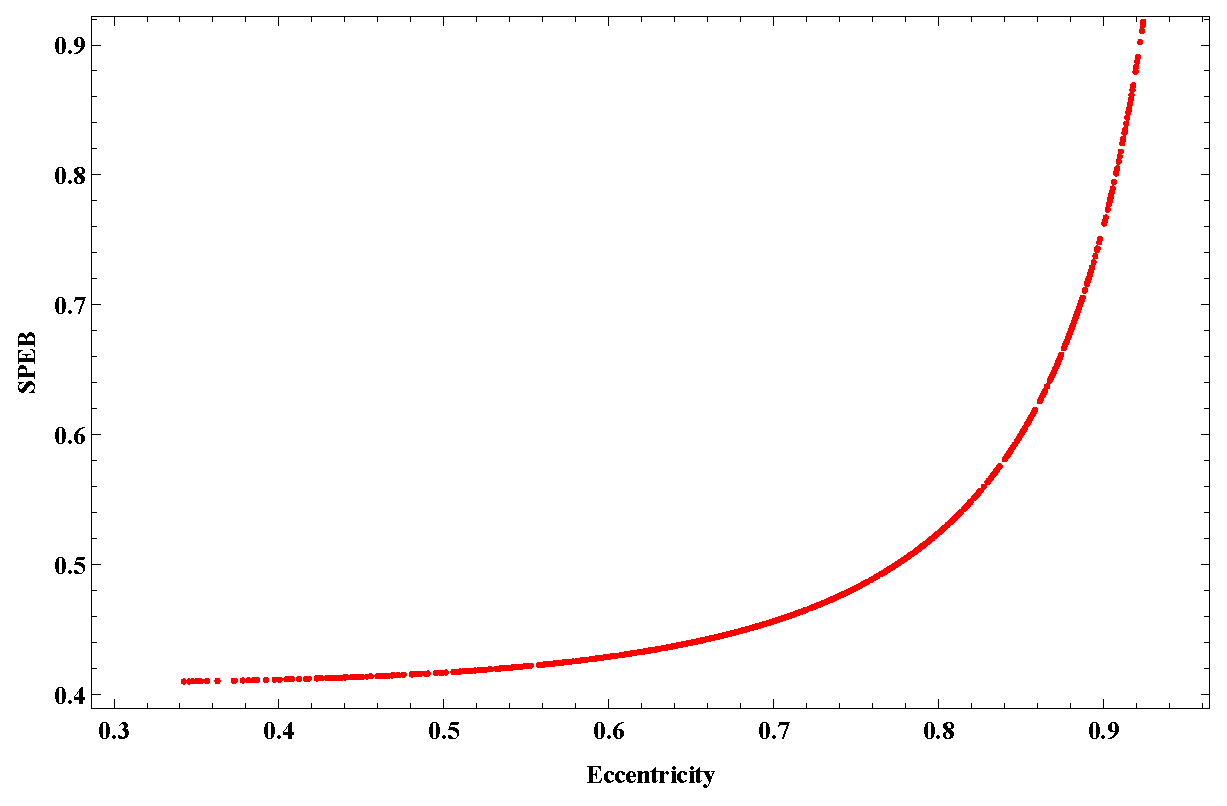
\includegraphics[width=400pt]{eccentricity_SPEB.eps}
  \caption{SPEB与信息椭圆离心率的关系}\label{fig:eccentricity}
\end{figure}
从图\ref{fig:eccentricity}可以看出:
\begin{itemize}
  \item 定位误差下界在$\lambda_i$给定的情况下完全由椭圆离心率决定,如果我们联立$e=\sqrt{1-\lambda_{\min}/\lambda_{\max}}$与式(\ref{eq:Lambda}),式(\ref{eq:SPEB_min})不难得出这个结论
  \item 定位误差下界是椭圆离心率的增函数,这与式(\ref{eq:SPEB_min})相吻合。在椭圆离心率比较小的情况下,误差下界已经接近$e=0$时的$1/\sum \lambda_i=0.408$。
\end{itemize}
\end{remark}
\section{两个未知节点协作的场景}\label{section:two_node_cooperation}
两个移动节点协作情况下,为求4维费舍尔信息矩阵特征多项式的表达式,需要下面的定理:
\begin{theorem}\label{thm:ShenIden}
设$J$是对称正定的矩阵,那么下式成立:
\begin{equation}\label{eq:ShenIden}
|J+\epsilon \bm{u}\bm{u}^{\textrm{T}} |=|J|+\epsilon \bm{u}^{\textrm{T}} J^*\bm{u}
\end{equation}
其中$J^*$表示J的伴随矩阵,满足等式$JJ^*=|J|\bm{I}$。
\end{theorem}
证明上面的定理需要如下两个引理:
\begin{lemma}\cite{aa}\label{lemma:block}
如果方阵$\bm{M}$可以写成分块的形式$\left(\begin{array}{cc}
A&B\\
C&D\\
\end{array}\right)$,而且A是可逆的对角阵,那么$\bm{M}$的行列式$|\bm{M}|=|A||D-CA^{-1}B|$
如果方阵$\bm{M}$可以写成分块的形式$\left(\begin{array}{cc}
A&B\\
C&D\\
\end{array}\right)$,而且A是可逆的对角阵,那么$\bm{M}$的行列式为
\begin{equation}
|\bm{M}|=|A||D-CA^{-1}B|.
\end{equation}
\end{lemma}
\begin{proof}
通过第三类初等变换方阵我们有
\begin{equation}
\left(\begin{array}{cc}
I&0\\
-CA^{-1}&I\\
\end{array}\right) \bm{M}=\left(\begin{array}{cc}
A&B\\
0&D-CA^{-1}B\\
\end{array}\right)
\end{equation}
两边同时取行列式即得要证明的式子。
\end{proof}

\begin{lemma}
如果$\bm{u}$是一个n维的列向量,$\bm{I}$是n维单位阵,则我们有行列式恒等式:
\begin{equation}\label{eq:con_eq}
|(1+\bm{u}^{\textrm{T}} \bm{u})\bm{I}-\bm{u}\bm{u}^{\textrm{T}} |=(1+\bm{u}^{\textrm{T}} \bm{u})^{n-1}.
\end{equation}
\end{lemma}
证明(\ref{eq:con_eq})需要下面的Woodbury 矩阵求逆公式:
\begin{equation}\label{eq:woodbury}
(A+UCV)^{-1}=A^{-1}-A^{-1}U(C^{-1}+VA^{-1}U)^{-1}VA^{-1}
\end{equation}
其中A,C均是可逆的方阵。


\begin{proof}
用数学归纳法证明,首先我们对$n=2$的情形直接验证可得(\ref{eq:con_eq})成立。
假设结论对n-1维的情形成立,设$\bm{u}=(\bm{v}^{\textrm{T}} ,u_n)^{\textrm{T}} $,其中$\bm{v}$是n-1维的列向量,那么对$\bm{v}/\sqrt{1+u_n^2}$用归纳假设有:
\begin{equation}
|(1+\frac{||\bm{v}||^2}{1+u_n^2})\bm{I}_{n-1}-\frac{\bm{v}\bm{v}^{\textrm{T}} }{1+u_n^2}|=(1+\frac{||\bm{v}||^2}{1+u_n^2})^{n-2}
\end{equation}
其中,$||\bm{v}||^2=\bm{v}^{\textrm{T}} \bm{v},||\cdot||$表示欧式空间的2范数。
由上式可得:
\begin{align*}
\begin{cases}
A:&=(1+u_n^2+||\bm{v}||^2)\bm{I}_{n-1}-\bm{v}\bm{v}^{\textrm{T}}\\
|A|&=(1+u_n^2)(1+u_n^2+||\bm{v}||)^{n-2}.
\end{cases}
\end{align*}
对n维的情形,$(1+\bm{u}^{\textrm{T}} \bm{u})\bm{I}-\bm{u}\bm{u}^{\textrm{T}} $可以写成分块矩阵的形式$\left(\begin{array}{cc}
A&-u_n\bm{v}\\
-u_n\bm{v}^{\textrm{T}} &||\bm{v}||^2+1\\
\end{array}\right)$。
由引理(\ref{lemma:block})得:
\begin{equation}\label{eq:LMidd}
|(1+\bm{u}^{\textrm{T}} \bm{u})\bm{I}-\bm{u}\bm{u}^{\textrm{T}} |=|A|(||\bm{v}||^2+1-u_n^2 \bm{v}^{\textrm{T}} A^{-1}\bm{v}).
\end{equation}
由Woodbury矩阵求逆公式:
\begin{equation}\label{eq:AInv}
A^{-1}=\frac{1}{1+||\bm{v}||^2+u_n^2}-\frac{\bm{v}(-1+||\bm{v}||^2/(1+||\bm{v}||^2+u_n^2))^{-1}\bm{v}^{\textrm{T}} }{(1+||\bm{v}||^2+u_n^2)^2}.
\end{equation}
将(\ref{eq:AInv})代入(\ref{eq:LMidd})中,化简即可得对n的情形要证的恒等式成立。
\end{proof}

\begin{proof}[定理(\ref{thm:ShenIden})证明]
式(\ref{eq:ShenIden})等价于:
\begin{equation}\label{eq:ShenIden_1}
|J+\epsilon \bm{u}\bm{u}^{\textrm{T}} |=|J|(1+\epsilon \bm{u}^{\textrm{T}} J^{-1}\bm{u}).
\end{equation}
因为J是对称正定的矩阵,所以存在正交矩阵Q,使得$J=QDQ^{-1}$,D是对角阵,
代入(\ref{eq:ShenIden_1})中得:
$|D+\epsilon \bm{y}\bm{y}^{\textrm{T}} |=|D|(1+\epsilon \bm{y}^{\textrm{T}} D^{-1}\bm{y})$
其中$\bm{y}=Q^{-1}\bm{u}$,因此我们只需对对角矩阵证明定理成立。
设J是n维对角阵,由Woodbury矩阵恒等式可得:
\begin{equation}
(J+\epsilon \bm{u}\bm{u}^{\textrm{T}} )^{-1}=J^{-1}-\frac{1}{\epsilon^{-1}+\bm{u}^{\textrm{T}} J^{-1}\bm{u}}J^{-1}\bm{u}\bm{u}^{\textrm{T}} J^{-1}.
\end{equation}
整理得:
\begin{equation}\label{eq:ShenIden_2}
(J+\epsilon \bm{u}\bm{u}^{\textrm{T}} )^{-1}=J^{-1}\frac{(1+\epsilon\bm{u}^{\textrm{T}} J^{-1}\bm{u})\bm{I}-\epsilon \bm{u}\bm{u}^{\textrm{T}} J^{-1}}{1+\epsilon\bm{u}^{\textrm{T}} J^{-1}\bm{u}}.
\end{equation}
如果我们能证明:
\begin{equation}
|(1+\epsilon\bm{u}^{\textrm{T}} J^{-1}\bm{u})\bm{I}-\epsilon \bm{u}\bm{u}^{\textrm{T}} J^{-1}|=(1+\epsilon\bm{u}^{\textrm{T}} J^{-1}\bm{u})^{n-1}
\end{equation}
则通过对(\ref{eq:ShenIden_2})两边取行列式即可得到要证的式子,这里设$J=\text{diag}(\lambda_1,...\lambda_n)$,取$y=\sqrt{\epsilon}(u_1/\sqrt{\lambda_1},...u_n/\sqrt{\lambda_n})$,那么上式和(\ref{eq:con_eq})具有相同的形式,因此定理结论成立。
\end{proof}
定理(\ref{thm:ShenIden})可以推广为如下一般形式,证明方法同上。
\begin{corollary}设$J$是对称正定的矩阵,则
\begin{equation}
|J+\epsilon \bm{u}\bm{v}^{\textrm{T}} |=|J|+\epsilon \bm{u}^{\textrm{T}} J^*\bm{v}.
\end{equation}
\end{corollary}
下面我们利用定理(\ref{thm:ShenIden})考虑两个节点协作的情形:
原4维FIM结构为:
\begin{equation}
A=\left(\begin{array}{cc}
\bm{\Sigma}_0+\epsilon \bm{u}\bm{u}^{\textrm{T}}  &-\epsilon \bm{u}\bm{u}^{\textrm{T}}  \\
-\epsilon \bm{u}\bm{u}^{\textrm{T}}  & \bm{\Sigma}_1+\epsilon \bm{u}\bm{u}^{\textrm{T}}
\end{array}
\right).
\end{equation}
通过坐标变换将$\bm{\Sigma}_0,\bm{\Sigma}_1$对角化可以得到等价的形式:
\begin{equation}
A=J+\epsilon\binom{\bm{v}}{-\bm{w}}(\bm{v}^{\textrm{T}} ,-\bm{w}^{\textrm{T}} )
\end{equation}
其中$v,w$为单位方向向量,方向角为$\theta$和$\phi$。而J是对角矩阵,第i个对角元为$\lambda_i$,这样特征多项式$|\lambda A-I|=0$就有简单的表达形式:

\begin{equation}\label{eq:4_characteristic_polynomial}
P(\lambda)= (\lambda-a_1)(\lambda-a_2)(\lambda-a_3)(\lambda-a_4)(1+\epsilon(\frac{\cos^2(\theta)}{\lambda-a_1}+
 \frac{\sin^2(\theta)}{\lambda-a_2}+\frac{\cos^2(\phi)}{\lambda-a_3}+\frac{\sin^2(\phi)}{\lambda-a_4})).
\end{equation}
利用SPEB的定义和式(\ref{eq:4_characteristic_polynomial}),可以得到相比于非协作的情形定位误差下界下降的成分为:
\begin{equation}
\Delta=\sum \frac{1}{\lambda_i}-\text{SPEB}_{\text{global}}=\xi\left(\frac{\cos^2(\theta)}{a_1^2}+\frac{\sin^2(\theta)}{a_2^2}+\frac{\cos^2(\phi)}{a_3^2}+\frac{\sin^2(\phi)}{a_4^2}\right)
\end{equation}
其中
\begin{equation}
\xi=\left(\frac{1}{\epsilon}+\frac{\cos^2(\phi)}{a_3}+\frac{\sin^2(\phi)}{a_4}+\frac{\cos^2(\theta)}{a_1}+\frac{\sin^2(\theta)}{a_2}\right)^{-1}.
\end{equation}
考察上面关于$\theta$和$\phi$的函数,我们有如下定理,推导过程见附录[\ref{B_F_0}]:
\begin{theorem}\label{theorem:2node_in_cooperation}
如果$\frac{1}{a_1}+\frac{1}{a_2}\geq \max\{\frac{1}{a_4},\frac{1}{a_3}\}$且$\frac{1}{a_3}+\frac{1}{a_4}\geq\max\{\frac{1}{a_1},\frac{1}{a_2}\}$,那么$\theta=\phi=\frac{\pi}{2}$是$\Delta$的最大值点。
\end{theorem}
\section{本章小结}\label{section:conclusion3}
  % Keep the summary *very short*.
  我们在本章中针对简单网络研究了通过改变角度参数使得误差下界最小这一问题,现总结如下:
  \begin{itemize}
  \item 对于非协作情形,如果能改变锚点部署的角度使得费舍尔信息矩阵是对角阵(信息椭圆退化成圆),则误差下界最小,但根据图\ref{fig:eccentricity}的结果,仿真1000次大部分情况下椭圆离心率在0.4以上,因此信息椭圆退化成圆只是一个理论最优的结果,实际系统很难达到。
  \item 对于两节点协作的情形,定理\ref{theorem:2node_in_cooperation}给出了一个充分条件以确定定位误差最小的情形。
  \end{itemize}


  尽管锚点贡献的信息椭圆在实际中很难退化成圆,但从\ref{section:two_node_cooperation}小节的推导来看,锚点贡献的信息是各向异性的情况下作理论推导会非常困难,文献\cite{LimitBound3}给出了三个节点协作场景下定位误差下界一般的表达式,但对于更多节点协作的情形,如果我们关心协作信息的特性,不妨简化锚点贡献的信息为各向同性的,这样做一方面是出于进一步理论分析的方便同时又不影响要研究的主要问题。
  因此在接下来的研究中,我们总是假设式(\ref{eq:general_fim})中出现的$I(\bm{p}_i)$是形如$c\bm{I}_2$的对角阵。
  在接下来的研究工作中我们会采用不同于\ref{section:two_node_cooperation}小节的数学方法来求解费舍尔信息矩阵的特征值。

\chapter{特殊结构网络}\label{cha:content4}
\section{特殊的全连接网络}\label{section:complete_graph_cooperation}
在协作定位网络的问题模型下,给出下面三个简化条件:
\begin{enumerate}
\item 锚点测距方差$\sigma_i^2=\frac{1}{a}$;
\item 未知节点彼此测距方差$\sigma^2_{ij}=\frac{1}{b}$;
\item $\mathcal{E}=\{(i,j)|1\leq i <j\leq N\},N:=N_a,\angle\bm{u}_j=\frac{2\pi j}{n}$。
\end{enumerate}
$\bm{I}(\bm{P})$的最大特征值和最小特征值可由\textbf{瑞利商}求出,关于瑞利商有如下定理:
\begin{theorem}\label{theorem:rayleigh}
  设$\bm{A}$是一个对称正定的矩阵,设$\bm{v}_{\lambda}$为A的特征值$\lambda$对应的特征向量,则:
\begin{align*}
\begin{cases}
\lambda_{\text{max}}&=\max_{||\bm{x}||=1} \transpose{\bm{x}}\bm{A}\bm{x}\\
\bm{v}_{\lambda_{\text{max}}}&=\rgmax_{||\bm{x}||=1} \transpose{\bm{x}}\bm{A}\bm{x}
\end{cases}\\
\begin{cases}
\lambda_{\text{min}}&=\min_{||\bm{x}||=1} \transpose{\bm{x}}\bm{A}\bm{x}\\
\bm{v}_{\lambda_{\text{min}}}&=\rgmin_{||\bm{x}||=1} \transpose{\bm{x}}\bm{A}\bm{x}.
\end{cases}
\end{align*}
\end{theorem}

在条件(1),(2)成立的情况下,费舍尔信息矩阵$I(\bm{p}_1,\dots,\bm{p}_N)=a\bm{I}_{2N}+b\bm{J}$,其中
\begin{equation}
\bm{J}_{ij}=\begin{cases}
\sum_{k=1,k\neq i}^N \bm{u}_{ik}\bm{u}_{ik}^{\textrm{T}} &i=j\\
-\bm{u}_{ij}\bm{u}_{ij}^{\textrm{T}} &i\neq j.
\end{cases}
\end{equation}
瑞利商为:
\begin{equation}
R(\bm{x})=b\sum_{i\leq j\leq N} (\bm{u}_{ij}^{\textrm{T}} (\bm{x}_i-\bm{x}_j))^2+a,\bm{x}_i\in \mathbb{R}^2
\end{equation}
当$\bm{x}_i=\bm{x}_j$或$(\bm{x}_i-\bm{x}_j)$与$\bm{u}_{ij}$正交时,瑞利商$R(\bm{x})$取到最小值,
利用定理(\ref{theorem:rayleigh}),关于$I(\bm{p}_1,\dots,\bm{p}_N)$的特征值,我们有如下定理:
\begin{theorem}
如果简化条件1和2成立,那么$I(\bm{p}_1,\dots,\bm{p}_N)$的最大特征值是$a+Nb$,最小特征值是a;
如果三个简化条件均成立,那么$\mathbb{R}_{2N}=V_{a+Nb}\oplus V_a\oplus V_{a+Nb/2}$,且$dim(V_a)=3,dim(V_{a+Nb/2})=2N-4$.
\end{theorem}
\begin{proof}
设$\mathring{p}_i$表示$\bm{p}_i$绕原点旋转$90^{\circ}$后的向量,$\bm{e}_1=(1,0),\bm{e}_2=(0,1)$,
则有
\begin{equation}
V_a \supset\text{span}\{\{\bm{\mathring{p}_1},\bm{\mathring{p}_2},\dots,\bm{\mathring{p}} _N\},\{\bm{e}_1,\bm{e}_1,\dots,\bm{e}_1\},\{\bm{e}_2,\bm{e}_2,\dots,\bm{e}_2\}\}:=K_a.
\end{equation}
下面证明$a+Nb$是$I(\bm{p}_1,\dots,\bm{p}_N)$的最大特征值,由Cauchy不等式:
\begin{align}\notag
R(\bm{y})&\leq b\sum_{i\leq j\leq N} ||\bm{u}_{ij}||^2||\bm{y}_i-\bm{y}_j||^2+a\\
&=b\sum_{i\leq j\leq N}||\bm{y}_i-\bm{y}_j||^2+a
\end{align}
取等条件是$\forall i,j\in \{1,2,...N\},i\neq j$,有$\bm{y}_i-\bm{y}_j$与$\bm{u}_{ij}$均平行,比如可以取
$\bm{y}_1-\bm{y}_j=k(\bm{p}_1-\bm{p}_j),j=2,...N$。
满足
$\bm{y}_i-\bm{y}_j=(\bm{y}_1-\bm{y}_j)-(\bm{y}_1-\bm{y}_i)
=k(\bm{p}_i-\bm{p}_j)\parallel \bm{u}_{ij}$。
这时原来2N个自由度的y还剩下$\bm{y}_1$和k三个自由度,考虑条件极值
$f(\bm{y})=\sum_{i\leq j\leq N} ||\bm{y}_i-\bm{y}_j||^2,\text{s.t } ||\bm{y}||=1$。
设矩阵T为:
\begin{equation}
\bm{T}=\left(
\begin{array}{cccc}
(N-1)\bm{I}_2&-\bm{I}_2&\dots&-\bm{I}_2\\
-\bm{I}_2&(N-1)\bm{I}_2&\dots&-\bm{I}_2\\
\vdots & \vdots & \ddots & \vdots\\
-\bm{I}_2& -\bm{I}_2 & \dots & (N-1)\bm{I}_2
\end{array}
\right)
\end{equation}
$\bm{T}$可以写成$\bm{T}=N\bm{I}-\bm{e}\bm{e}^{\textrm{T}} $,其中$\bm{e}=(\bm{I}_2,\dots,\bm{I}_2)^{\textrm{T}} $。而$f(\bm{y})=\bm{y}^{\textrm{T}} \bm{T}\bm{y}=N-(\bm{e}^{\textrm{T}} \bm{y})^{\textrm{T}} (\bm{e}^{\textrm{T}} \bm{y})\leq N$,取等条件是$\bm{e}^{\textrm{T}} \bm{y}=\bm{0}$。这个条件限制住了两个自由度,再加上$\bm{y}$模长为1的约束,前一次不等式取等剩下的三个自由度刚好够用,
所以$\bm{y}$按该方法可以唯一取到,其张成的子空间记为$K_b$。
具体求解可得
$\bm{y}_1=\frac{k}{N}\sum_{j=2}^N (\bm{p}_1-\bm{p}_j)$。
将$\bm{y}_i$的表达式代入$||\bm{y}||=1$中,可以解出唯一的$k^2=M$,
其中
\begin{equation}
M\sum_{i=1}^N||\sum_{j=1,j\neq i}^N(\bm{p}_1-\bm{p}_j)||^2=1.
\end{equation}
  在条件(3)$\angle\bm{u}_j=\frac{2\pi j}{n}$的进一步假设下,设$\bm{x}\in (K_a\oplus K_b)^{\bot}$,
  下面证明$\bm{x}$是矩阵$\bm{J}$的特征值为$\frac{N}{2}$对应的特征向量。
  由正交性条件,有:
\begin{align}
\begin{cases}
\sum \bm{x}_i^{(k)}&=0,k=1,2\\
\sum \bm{x}_i \cdot \bm{u}_i&=\sum x_i^{(1)} \cos(\frac{2\pi j}{n})+x_i^{(2)} \sin(\frac{2\pi j}{n})=0
\label{eq:coupling1}\\
\sum \bm{x}_i \cdot \mathring{\bm{u}}_i &=\sum -x_i^{(1)} \sin(\frac{2\pi j}{n})+x_i^{(2)} \cos(\frac{2\pi j}{n}) =0
\end{cases}
\end{align}
下面考虑$\bm{K}\cdot \bm{x}$的第j行为:
\begin{equation}\label{eq:tt}
\left(\bm{K}\cdot \bm{x}\right)_{(\cdot,j)}=\sum_{k\neq j}^n \frac{(\bm{u}_j-\bm{u}_k)^{\textrm{T}} (\bm{x}_j-\bm{x}_k)}{||\bm{u}_j-\bm{u}_k||^2}(\bm{u}_j-\bm{u}_k).
\end{equation}
我们要证明上面的式子等于$\frac{N}{2}\bm{x}_j$,为此,首先化简$(\bm{u}_j-\bm{u}_k)/||\bm{u}_j-\bm{u}_k||$有
\begin{equation}
\frac{(\bm{u}_j-\bm{u}_k)}{||\bm{u}_j-\bm{u}_k||}=\text{sgn}(j-k)\binom{-\sin\frac{\pi(j+k)}{n}}{\cos\frac{\pi(j+k)}{n}}.
\end{equation}
上面的式子中符号函数$\text{sgn}(j-k)$因为在式(\ref{eq:tt})中出现2次,所以相乘恒为1,它与求和指标k无关,可以作为公因子提取出来。
所以证明\begin{equation}
\sum_{k\neq j}^n \frac{(\bm{u}_j-\bm{u}_k)^{\textrm{T}} (\bm{x}_j-\bm{x}_k)}{||\bm{u}_j-\bm{u}_k||^2}(\bm{u}_j-\bm{u}_k)=\frac{N}{2}\bm{x}_j
\end{equation}
化简为分别证明:
\begin{align*}\label{eq:star1}
\sum ((-\sin\frac{(j+k)\pi}{n},\cos\frac{(j+k)\pi}{n})\binom{x_j^{(1)}-x_k^{(1)}}{x_j^{(2)}-x_k^{(2)}})
\cos\frac{(j+k)\pi}{n}&=\frac{N}{2}x_j^{(2)}\\
\sum ((-\sin\frac{(j+k)\pi}{n},\cos\frac{(j+k)\pi}{n})\binom{x_j^{(1)}-x_k^{(1)}}{x_j^{(2)}-x_k^{(2)}})
(-\sin\frac{(j+k)\pi}{n})&=\frac{N}{2}x_j^{(1)}
\end{align*}
式(\ref{eq:star1})第一个等式等价于证明:
\begin{equation}
\sum (-\sin\frac{(j+k)2\pi}{n},1+\cos\frac{(j+k)2\pi}{n})\binom{x_j^{(1)}-x_k^{(1)}}{x_j^{(2)}-x_k^{(2)}}=Nx_j^{(2)}.
\end{equation}
在式(\ref{eq:coupling1}))中,将式(\ref{eq:coupling1})中第二个等式乘以$\sin(\frac{2\pi k}{n})$与第三个等式乘以$\cos(\frac{2\pi k}{n})$相减得:
\begin{equation}
\sum x_i^{(1)}\sin\frac{(j+k)2\pi}{n}-x_i^{(2)}\cos\frac{(j+k)2\pi}{n}=0.
\end{equation}
利用上面这个等式即可证式(\ref{eq:star1})第一个等式。
在式(\ref{eq:coupling1}))中,将式(\ref{eq:coupling1})中第二个等式乘以$\cos(\frac{2\pi k}{n})$与第三个等式乘以$\sin(\frac{2\pi k}{n})$相加得:
\begin{equation}
\sum x_i^{(1)}\cos\frac{(j+k)2\pi}{n}+x_i^{(2)}\sin\frac{(j+k)2\pi}{n}=0.
\end{equation}
利用上面这个等式同理可证明式(\ref{eq:star1})第二个等式。
\end{proof}
\begin{remark}

\begin{itemize}
~\\
  \item 当场景中各待测节点相距较近,而锚点离各待测节点较远时,\ref{section:circle_general}小节说明了各向同性是锚点最优部署的形态,如果考虑锚点相对于各待测节点的分布范围是最优部署的,那么上面对锚点部署使得其贡献的信息量为$a\bm{I}$的假设成立,在之后的讨论中,我们均持此假设。
  \item 假设3是说各待测节点分布在一个圆上,因为各待测节点相距较近,在圆周半径不是很小的情况下,可以近似认为各节点相互测距方差均相等,即假设2成立。
  \item 通过对特征值的倒数和取平均,每个节点的误差下界的量级是$\frac{4}{bN}$,\ref{section:circle_general}小节最优部署下非协作情形每个节点的误差下界的量级是$\frac{2}{aN}$,相比之下可以看出在a=b的情况下增加2个协作节点才达到一个锚点的效果。
\end{itemize}

\end{remark}
\section{线型网络}\label{section:linear_network}
在动态协作定位网络的问题模型下,得到的费舍尔信息矩阵是块三对角矩阵,在时间段[0,T]内,为研究减小时间间隔对定位性能的提高,我们需要对原来的模型作出如下的简化:
\begin{itemize}
\item 锚点测距方差$\sigma_i^2=\frac{1}{a}$,
\item 未知节点彼此测距方差$\sigma^2_{ij}=\frac{1}{b}$。
\end{itemize}
那么费舍尔信息矩阵式(\ref{eq:time_cooperation_matrix})可化简为
\begin{equation}\label{eq:Pab}
I(\bm{P})=a\bm{I}+b\bm{J}.
\end{equation}
其中\begin{equation}
J=\left(
\begin{array}{ccccc}
\bm{u}_{1}\bm{u}_{1}^{\textrm{T}} &-\bm{u}_{1}\bm{u}_{1}^{\textrm{T}} &\bm{0}&\dots&\bm{0}\\
&&&&\\
-\bm{u}_{1}\bm{u}_{1}^{\textrm{T}} &\bm{u}_{1}\bm{u}_{1}^{\textrm{T}} +\bm{u}_{2}\bm{u}_{2}^{\textrm{T}} &-\bm{u}_{2}\bm{u}_{2}^{\textrm{T}} &\dots&0\\
&&&&\\
\vdots &\vdots&\ddots &\vdots&\vdots\\
\bm{0}&\dots&\bm{0}&-\bm{u}_{N-1}\bm{u}_{N-1}^{\textrm{T}} &\bm{u}_{N-1}\bm{u}_{N-1}^{\textrm{T}} \\
\end{array}
\right).
\end{equation}
并且$u_i:=u_{i,i+1}$,
我们可以用$\lim_{N\to \infty}\frac{\Tr(J^{-1})}{N}$来表征节点的各个时刻的位置平均定位误差下界,下面我们试图通过特征值的方法求出这一极限。


直接求解该问题需要如下两个引理:
\begin{lemma}\label{lemma:change}
设L是$m\times n$的矩阵,$a,\epsilon > 0$则
\begin{equation}
|a\bm{I}_m+\epsilon \bm{L}\bm{L}^{\textrm{T}} |=a^m|\bm{I}_n+\frac{\epsilon}{a} \bm{L}^{\textrm{T}} \bm{L}|.
\end{equation}
\end{lemma}
\begin{proof}
不妨设$a=\epsilon=1$,
考虑到
\begin{equation}
\left(\begin{array}{cc}
\bm{I}_n+\bm{L}^{\textrm{T}} \bm{L}&\bm{0}\\
\bm{L}&\bm{I}_m\\
\end{array}\right)\sim\left(\begin{array}{cc}
\bm{I}_n&-\bm{L}^{\textrm{T}} \\
\bm{L}&\bm{I}_m\\
\end{array}\right)\sim\left(\begin{array}{cc}
\bm{I}_n&-\bm{L}^{\textrm{T}} \\
0&\bm{I}_m+\bm{L}\bm{L}^{\textrm{T}} \\
\end{array}\right).
\end{equation}
其中$\sim$表示矩阵相抵,两边取行列式即得$|\bm{I}_m+\bm{L}\bm{L}^{\textrm{T}} |=|\bm{I}_n+\bm{L}^{\textrm{T}} \bm{L}|$,证毕。
\end{proof}


\begin{lemma}\label{lemma:special}
$\bm{S}$是一个n-1维的方阵,\begin{equation}
\bm{S}=\left(
\begin{array}{cccc}
0&1&\dots&0\\
1&0&\dots&0\\
\vdots&\vdots&\ddots&\vdots\\
0&\dots&1&0\\
\end{array}\right).
\end{equation}则$\bm{S}$的n-1个特征值为:
\begin{equation}
\lambda_j=2\cos(\frac{\pi j}{n}),j=1,2,...,n-1.
\end{equation}
\end{lemma}
\begin{proof}
首先可以用数学归纳法证明S的特征多项式有递推公式:\begin{equation}
P_n(\lambda)=\lambda P_{n-1}(\lambda)-P_{n-2}(\lambda)
\end{equation}
其中$P_n(\lambda)$对应n维的S。
其次证明
\begin{equation}
U_n(\lambda)=\frac{1}{\sqrt{1-(\frac{\lambda}{2})^2}}\sin((n+1)\arccos(\frac{\lambda}{2}))
\end{equation}
适合上面的递推关系式。
最后证明$U_n(\lambda)$是关于$\lambda$的多项式,而这只需要证明$U_1(\lambda),U_2(\lambda)$是多项式即可。
\end{proof}

$\bm{I}(\bm{p}_1,\dots,\bm{p}_N)$的特征多项式为\begin{equation}
p(\lambda)=|(\lambda-a)\bm{I}-b\bm{L}\bm{L}^{\textrm{T}} |
\end{equation}
其中L是2N乘以N的矩阵:
\begin{equation}
L=\left(
\begin{array}{ccccc}
\bm{u}_1&0&\dots&&0\\
-\bm{u}_1&\bm{u}_2&0&\dots&0\\
0&-\bm{u}_2&\bm{u}_3&\dots&0\\
\vdots &\vdots&&\ddots &\vdots\\
0&\dots&0&-\bm{u}_{N-1}&0\\
\end{array}
\right).
\end{equation}
为获得该多项式的全部零点,我们进一步设$u_i=(1,0)^{\textrm{T}} $,即目标节点作直线运动,后面可以看到直线运动对应着误差最小的情形。
根据引理(\ref{lemma:change}),
\begin{equation}
|(\lambda-a)\bm{I}-bLL^{\textrm{T}} |=(\lambda-a)^{2N}|\bm{I}_n-\frac{b}{\lambda-a}L^{\textrm{T}} L|
\end{equation}
其中$L^{\textrm{T}} L$是N阶方阵:
\begin{equation}
L^{\textrm{T}} L=\left(
\begin{array}{ccccc}
2&-1&\dots&&0\\
-1&2&-1&\dots&0\\
0&-1&2&\dots&0\\
\vdots &\vdots&&\ddots &\vdots\\
0&\dots&&0&0\\
\end{array}
\right).
\end{equation}
设$\bm{K}_{N-1}$为$L^{\textrm{T}} L$第N-1阶主子式,则
\begin{equation}
|(\lambda-a)\bm{I}-bLL^{\textrm{T}} |=(\lambda-a)^{N+1}|(\lambda-a)\bm{I}_{N-1}-b\bm{K}_{N-1}|.
\end{equation}
设$n:=N$,则$\bm{K}_{n-1}=2\bm{I}_{n-1}-\bm{S}$,由引理(\ref{lemma:special})可求出$\bm{I}(\bm{p}_1,\dots,\bm{p}_N)$的全部特征值。
\begin{equation}
f(n)=\frac{\Tr(J^{-1})}{n}==\frac{1}{n}\left(\frac{n+1}{a}+\sum_{j=1}^{n-1}\frac{1}{a+2b(1-\cos(\frac{\pi j}{n}))}\right)
\end{equation}
当$n\to \infty$,根据Riemann积分的定义:
\begin{equation}
\lim_{n\rightarrow \infty}f(n)=\frac{1}{a}+\int_0^1 \frac{1}{a+2b(1-cos(\pi x))}dx
\end{equation}
化为复积分由留数定理可得
\begin{equation}\label{eq:a24ab}
\lim_{n\rightarrow \infty}f(n)=\frac{1}{a}+\frac{1}{\sqrt{a^2+4ab}}.
\end{equation}

解析求解$\bm{I}(\bm{P})$的全部特征值在$\bm{u}_i$不共线时非常困难,在数值代数中针对三对角矩阵有追赶法(Thomas algorithm)来快速求解$A^{-1}b$\cite{numericalAnalysis},下面我们会推广这一方法使之适用于我们研究中的块三对角矩阵$\bm{I}(\bm{P})$。
%EFIM的思路是说,如果我们只关心场景中单个移动节点的定位误差,则可以通过分块矩阵的思路对总体的FIM进行分解。
首先注意到式(\ref{eq:Pab})中$a\bm{I}+b\bm{J}$可以提取b(相当于对b作归一化),记$\lambda=a/b$,下面我们针对$\lambda \bm{I}+\bm{J}$进行研究。

记
\begin{equation}
\bm{e}_i=(\bm{0},\dots,\underbrace{\bm{I}_2}_{\text{i-th item}},\dots,\bm{0})^{\textrm{T}}.
\end{equation}
在式(\ref{eq:SPEB_formula})中SPEB可以分解为各节点的定位误差下界之和为:
\begin{equation}\label{eq:SPEB_every_node}
  \text{SPEB}=\sum_{i=1}^{N_a} \bm{e}_i^{\textrm{T}}(\bm{I}(\bm{P}))^{-1}\bm{e}_i.
\end{equation}
$\bm{e}_i^{\textrm{T}}(\bm{I}(\bm{P}))^{-1}\bm{e}_i$是$(\bm{I}(\bm{P}))^{-1}\bm{e}_i$第i个2乘2的分块矩阵,
我们先考虑$i=N_a$即$\bm{e}_{N_a}$中只有最后一个块矩阵是2乘2的单位阵,其余位置都是零元。
$\bm{e}_{N_a}^{\textrm{T}}(\bm{I}(\bm{P}))^{-1}\bm{e}_{N_a}$表示终点位置的位置误差下界。
为记号简便,记$\bm{u}_{N_a}=\bm{0}$,$\bm{B}_i=\lambda\bm{I}+\bm{u}_i\bm{u}_i^{\textrm{T}}+\bm{u}_{i+1}\bm{u}_{i+1}^{\textrm{T}}$,$A_{i+1}=-\bm{u}_i\bm{u}_i^{\textrm{T}}$
则$\bm{I}(\bm{P})$可以写为:
\begin{equation}
\bm{I}(\bm{P})=\begin{pmatrix}
                 \bm{B}_1 & \bm{A}_2 & \bm{0} & \dots & \bm{0} \\
                 \bm{A}_2 & \bm{B}_2 & \bm{A}_3 & \dots & \bm{0} \\
                 \vdots & \vdots & \vdots & \ddots & \vdots \\
                 \bm{0} & \dots & \bm{0} & \bm{A}_{N_a} & \bm{B}_{N_a}
               \end{pmatrix}.
\end{equation}
$\bm{I}(\bm{P})$可以做LU分解如下:
\begin{equation}\label{eq:LU}
  \bm{I}(\bm{P})=\begin{pmatrix}
                 \bm{I}_2 & \bm{0} & \bm{0} & \dots & \bm{0} \\
                 \bm{L}_2 & \bm{I}_2 & \bm{0} & \dots & \bm{0} \\
                 \vdots & \vdots & \vdots & \ddots & \vdots \\
                 \bm{0} & \dots & \bm{0} & \bm{L}_{N_a} & \bm{I}_{2}
               \end{pmatrix}\begin{pmatrix}
                 \bm{U}_1 & \bm{A}_2 & \bm{0} & \dots & \bm{0} \\
                 \bm{0} & \bm{U}_2 & \bm{A}_3 & \dots & \bm{0} \\
                 \vdots & \vdots & \vdots & \ddots & \vdots \\
                 \bm{0} & \dots & \bm{0} & \bm{0} & \bm{U}_{N_a}
               \end{pmatrix}.
\end{equation}
$\bm{U}_i$满足如下递推关系:
\begin{equation}\label{eq:U_recursive_formula}
\begin{cases}
  \bm{U}_1 &= \bm{B}_1 \\
  \bm{U}_i &= \bm{B}_i-\bm{A}_i\bm{U}_{i-1}^{-1}\bm{A}_i,i\geq 2.
\end{cases}
\end{equation}
进一步可以求出
\begin{equation}\label{eq:thomas_final}
\bm{e}_{N_a}^{\textrm{T}}(\bm{I}(\bm{P}))^{-1}\bm{e}_{N_a}=U_{N_a}^{-1}.
\end{equation}
关于$U_{N_a}$的结构我们有如下定理:
\begin{theorem}
$U_{N_a}$一个特征值是$\lambda$,另一个特征值$T_1$可以用下面的递归方法得到
\begin{equation}\label{eq:recursive_efim}
\begin{split}
\underbrace{T_{i-1}-\lambda}_{M} & =\frac{1}{1+\frac{\sin^2\theta_i}{\lambda}+\frac{\cos^2\theta_i}{T_i}},2\leq i\leq N_a-1\\
T_{N_a-1} & = \lambda+\frac{1}{1+1/\lambda}
\end{split}
\end{equation}
其中$\theta_i=\measuredangle (u_{N_a +1-i},u_{N_a-i})$。
%Ti should be described by symbol, not natural language.
\end{theorem}
具体推导过程详见附录[\ref{B_F_1}]。
% \nonumber % Remove numbering (before each equation)
%\begin{definition}
%    设矩阵$I=\left(\begin{array}{cc}A&B\\C&D\end{array}\right)$,那么矩阵$I$关于D的Schur补定义为$
%    I/\ D=A-BD^{-1}C$,若$I^{-1}$与I作同样的分块,则$(I/\ D)^{-1}$是$I^{-1}$左上角的分块矩阵。
%\end{definition}
%\begin{remark}
%	在我们的应用场景中,矩阵$I$是费舍尔信息矩阵,可以证明$(I/\ D)$给出于参数空间$\Theta$的子空间的费舍尔信息矩阵,计算$\text{tr}(I^%{-1})$可以分解为计算各个子空间的误差再求和,一般取子空间的大小为2维,对应着一个位置的XY坐标。$I/\ D$在我们的应用场景中也称为等效费舍尔信%息矩阵(Equivalent Fisher Information Matrix)。
%\end{remark}
%{用Schur补求解节点平均定位误差}
\begin{remark}
终点的定位误差
\begin{equation}\label{eq:final_speb}
\text{SPEB}=\frac{1}{\lambda}+\frac{1}{T_1(N_a)}.
\end{equation}
强度量$\lambda$确定后,研究$N_a$增大对SPEB的影响归结为研究$T_1(N_a)$的性质,下面我们将采用连分式的数学方法研究$T_1(N_a)$关于$N_a\to \infty$的收敛性和收敛速度的问题,本文中用到的关于连分式的结论在附录[\ref{C_F}]中列出\cite{ContinuedFraction}:
\end{remark}
\begin{remark}

上述求解是针对目标节点的计时终点而言,计时起点完全类似。如果针对其时间中点,则其可分别看成两段轨迹的起点和终点,
可以推出其费舍尔信息矩阵为:
\begin{equation}
\bm{I}(\bm{p}_i)=\lambda I+M_1\bm{u}\bm{u}^{\textrm{T}} +M_2\bm{v}\bm{v}^{\textrm{T}}.
\end{equation}
其中$\bm{u}=\frac{\bm{p}_i-\bm{p}_{i-1}}{||\bm{p}_i-\bm{p}_{i-1}||}$,
$\bm{v}=\frac{\bm{p}_i-\bm{p}_{i+1}}{||\bm{p}_i-\bm{p}_{i+1}||}$,
$\phi=\measuredangle(\bm{u},\bm{v})$,
$M_1,M_2$分别作为各段轨迹的计时终点满足递推公式(\ref{eq:recursive_efim}),
$\bm{I}_p$的两个特征值为可由式(\ref{eq:Lambda})得出:
\begin{equation}\label{eq:time_interval_case}
\lambda_{1,2}=\lambda+\frac{M_1+M_2\pm \sqrt{M_1^2+M_2^2+2M_1M_2\cos2\phi}}{2}.
\end{equation}
注意到时间中点时两个特征值均比$\lambda$大。
%with no proof, because of time limit
\end{remark}
为解析地求出$\lim_{N_a\to \infty}T_1(N_a)$,我们先考虑所有$\bm{u}_i=(1,0)^{\textrm{T}} $的特殊情形,此时
\begin{align}\notag\label{eq:gcf_1}
\lim_{N_a\to \infty}T_1(N_a)=&\lambda+\cfrac{1}{1+\cfrac{1}{\lambda+\cfrac{1}{1+\cfrac{1}{\lambda+\dots}}}}\\
=&[\lambda,1,\lambda,1,\dots].
\end{align}
根据定理(\ref{theorem:quadratic_cyclic})我们可以求出
%先求循环的部分的连分式的值K,然后代入$\lambda+2/K$中即可
%K对应的迭代矩阵循环周期为2,
%写成$\begin{pmatrix}1 & 1 \\1 & 0\end{pmatrix}\begin{pmatrix}\lambda & 1 \\1 & 0\end{pmatrix}$
%解方程$x=\frac{(\lambda+1)x+1}{\lambda x+1}$并考虑到解$x>0$,得$K=\frac{\lambda+\sqrt{4\lambda+\lambda^2}}{2\lambda}$,
%最后得时间中点所求的目标节点的误差下界为$\sqrt{\lambda^2+4\lambda}$。同理,将式\ref{eq:gcf_1}中分子2改为1求出对应于时间起点或终点
误差下界为
\begin{equation}\label{eq:starting_or_ending}
M^*:=\lim_{N_a\to \infty}T_1(N_a)=\frac{\lambda+\sqrt{4\lambda+\lambda^2}}{2}.
\end{equation}
对于时间中点的情形,由式(\ref{eq:time_interval_case})可知其一个特征值为$\lambda$,另一个特征值:
\begin{align}\notag
\lambda_2=&\lambda+\frac{2}{[1,\lambda,1,\lambda,\dots]}\\
=&\lambda+\cfrac{2}{1+\cfrac{1}{\lambda+\cfrac{1}{1+\cfrac{1}{\lambda+\dots}}}}.
\end{align}
同样求出$\lambda_2=\sqrt{\lambda^2+4\lambda}$,这个结果与式(\ref{eq:a24ab})相一致。


从时间间隔终点位置误差下界的一般表达式可以看出:
\begin{enumerate}
  \item 根据式(\ref{eq:final_speb}),SPEB在一个方向上始终为$\frac{1}{\lambda}$,减小时间间隔也无法改善;
  \item 另一个方向上随$N_a$的增大$T_1(N_a)$会增大,但有一个上界,粗略的讲不可能超过$\lambda+1$
  \item 若某两次时间间隔夹角正交,则$\cos\theta_i=0$,即$t_i$时刻之前的所有位置均不能对终点位置的定位有贡献。
\end{enumerate}
对于一般的情形,当时间间隔比较小时,有理由假设角度不会有大的突变,且若轨迹的切向量如果是连续变化的,那么时间间隔充分小,前后两次测量间
角度可认为不变,那么有理由认为之前求的$M^*$是对一般的曲线轨迹在$\Delta t\to 0$时成立。因此我们有如下定理,证明可参考附录[\ref{B_F_6}]。
\begin{theorem}\label{theorem:arbitrary_curve}
若平面轨迹曲线参数化形式为$t\in[0,1]\rightarrow \bm{p}(t)=(x(t),y(t))$,满足
\begin{itemize}
\item $\bm{p}(t_1)\neq \bm{p}(t_2),\forall t_1\neq t_2$,
\item $\bm{p}'(t)$存在且连续。
\end{itemize}
对[0,1]区间有分割$0=t_1<t_2<\dots<t_{N_a-1}<t_{N_a}=1$,
记$\Delta t=\max_{1\leq i\leq N_a-1}|t_{i+1}-t_i|$
则式(\ref{eq:recursive_efim})给出的$T_1(N_a)$满足:
\begin{equation}\label{eq:limiting_cf}
\lim_{\Delta t\to 0}T_1(N_a)=M^*
\end{equation}
其中$M^*$在式(\ref{eq:starting_or_ending})中定义。
\end{theorem}

下面我们对不同的轨迹做数值计算,结果如图\ref{figure:tend_to_limit}所示
\begin{figure}
  \centering
  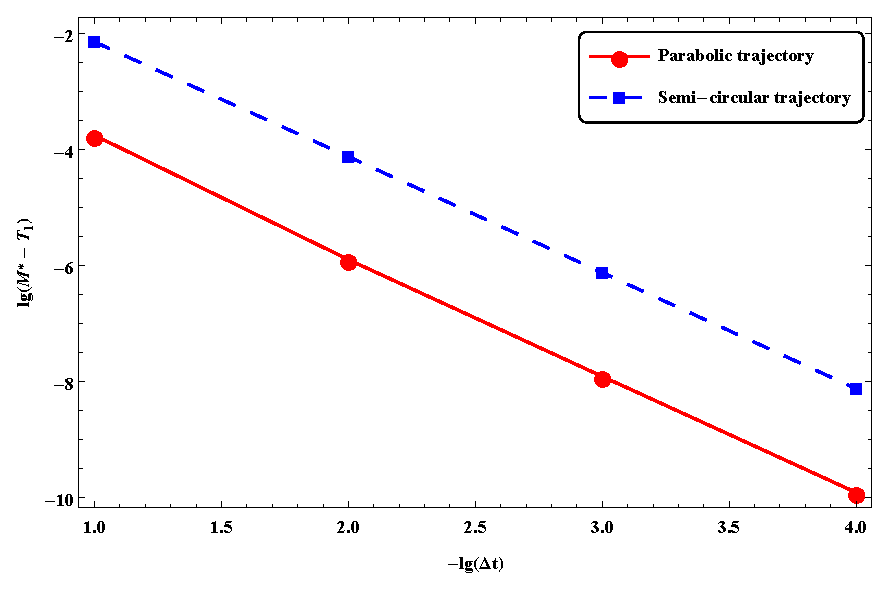
\includegraphics[width=400pt]{different_curve.eps}
  \caption{$\lambda=2$时不同曲线随采样点加密$T_1(N_a)$趋近极限值$M^*$的情况;其中抛物轨迹对应的曲线是$(t,t^2)$,半圆轨迹是$(\cos(\pi t),\sin(\pi t))$}\label{figure:tend_to_limit}
\end{figure}
%圆弧仿真

由图\ref{figure:tend_to_limit}可见,
\begin{itemize}
  \item 随着$\Delta t$的减小,各种曲线均二次收敛于极限值,二次收敛的结果可以从log-log图的斜率是1:2印证,
而从定理\ref{theorem:arbitrary_curve}的证明过程的式(\ref{eq:quatratic_convergence})中出现$\Delta t$的平方可见证明过程的合理性。
  \item 对于不同的曲线,虽然收敛速度的量阶一致,但由于角度变化上有快有慢,所以体现在图中还是有高有低,平均来说,半圆弧在一个时间单位中角度变化了180度,而抛物线只有不到60度,角度变化越小相对更接近直线状态,因而收敛地更快些。
\end{itemize}


虽然$\sqrt{\lambda^2+4\lambda}$是一个最大的信息量,但下面的定理指出,较远的时间间隔的位置的贡献实际上是幂指数衰减的,证明见附录[\ref{B_F_2}]。
\begin{theorem}\label{theorem:exponential_decreasing}
若相邻时间间隔最大的角度变化量小于$\Delta \theta$($\Delta \theta \leq \frac{\pi}{2}$),考虑在$t_1$时刻前的$t_0$时刻引入节点位置$\bm{p}_0$与$\bm{p}_1$有协作,这时由式(\ref{eq:recursive_efim})可计算出$T'_1(N_a)$大于原来的$T_1(N_a)$,记增量$\Delta_+ T_1(N_a):=T'_1(N_a)-T_1(N_a)$,$N_a=1$时有$\Delta_{+} T_{1}=\frac{\lambda}{\lambda+1}$,$N_a\geq 2$时$\Delta_+ T_1(N_a)$满足:
\begin{equation}
\frac{(\cos\Delta\theta)^{2(N_a-1)}}{(1+1/\lambda)^2(\lambda^2+2\lambda)(2+\lambda)^{2(N_a-2)}}\leq \Delta_+ T_1(N_a)\leq\frac{1}{(\lambda^2+2\lambda)(1+\lambda)^{2(N_a-2)}}.
\end{equation}
\end{theorem}
\begin{remark}

$T_1(N_a)$可看作终点位置沿信息椭圆长轴的费舍尔信息量,定理(\ref{theorem:exponential_decreasing})指出在距离终点费舍尔信息随链路是幂指数的衰减的,由于
\begin{align*}
  \Delta \text{SPEB}=&(\frac{1}{\lambda}+\frac{1}{T_1(N_a)})-(\frac{1}{\lambda}+\frac{1}{T_1(N_a)})\\
  =&\frac{\Delta_+ T_1(N_a)}{T_1(N_a)T'_1(N_a)}
\end{align*}
从而推出:
\begin{equation}
\frac{\Delta_+ T_1(N_a)}{(\lambda+1)^2}\leq  \Delta \text{SPEB} \leq \frac{\Delta_+ T_1(N_a)}{\lambda^2}
\end{equation}
所以误差下界的变化规律与$\Delta_{+} T_{1}$的规律一致,即我们得出了在时间协作的场景中的$N_a$条链路之外增加一层协作链路使目标节点定位误差的下降的数量是随$N_a$指数衰减的,因此在对某时刻的节点进行定位时,只需考虑其前后几个时刻的位置即可,较远的时刻基本没有信息量,利用上只会增加计算上的开销而对定位性能不会有多大的提升。
\end{remark}


为说明此结论,我们对式\ref{eq:recursive_efim}取不同的$\lambda$进行简单的数值计算,其中$\theta_i$按照~\ref{section:temporal_cooperative_localization}小节中$[0,2\pi]$均匀分布的假设求不同的$N_a$时$T_i$的性能平均,结果图~\ref{fig:continuous_fraction_exponential}所示。
\begin{figure}
  \centering
  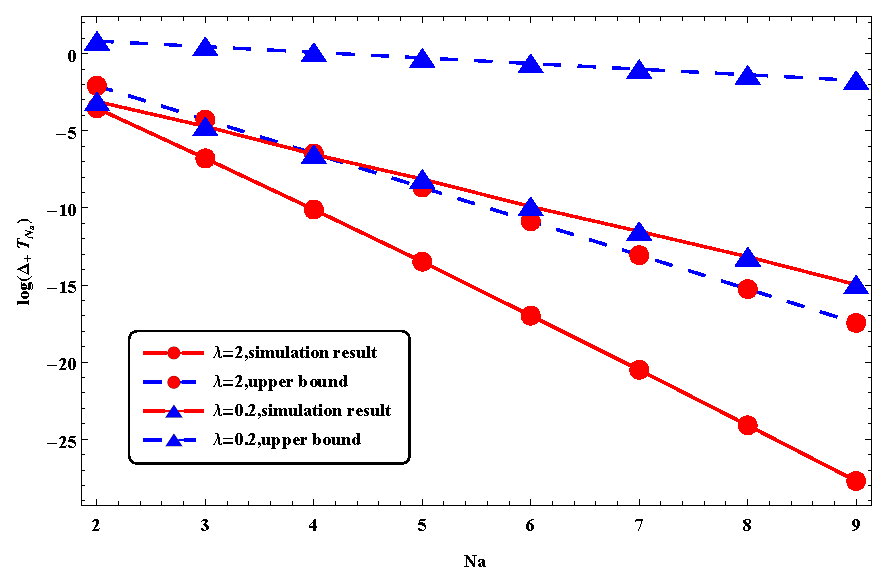
\includegraphics[width=400pt]{decreasing_exponential.eps}
  \caption{连分式指数收敛性图示}\label{fig:continuous_fraction_exponential}
\end{figure}
根据图~\ref{fig:continuous_fraction_exponential}可以看出:
\begin{itemize}
\item 通过蒙特卡罗仿真进一步验证了定理~\ref{theorem:exponential_decreasing}的正确性。
\item $\lambda=a/b$,表示锚点定位强度与目标节点协作强度之比,当$\lambda$较大即锚点定位更强时,图中协作信息量下降得更快,表明更远的协作链路所能提供的信息更少。
\item 实际随机模拟中的信息衰减速度要快于定理~\ref{theorem:exponential_decreasing}给出的上界,这主要是因为随机模拟中出现角度正交的情况时会阻断信息量从较远链路的传播。\end{itemize}

为了讨论信息衰减下界,我们取$\lambda=1$,并假设链路的夹角$\theta_i$服从零均值的正态分布,对于给定的$\Delta \theta$标准差$\sigma$满足$3\sigma=\Delta \theta$,由$3-\sigma$原则可近似认为角度变化不会超过$\Delta \theta$,数值结果如图\ref{fig:continuous_fraction_exponential_lower_bound}所示。
    \begin{figure}
      \centering
      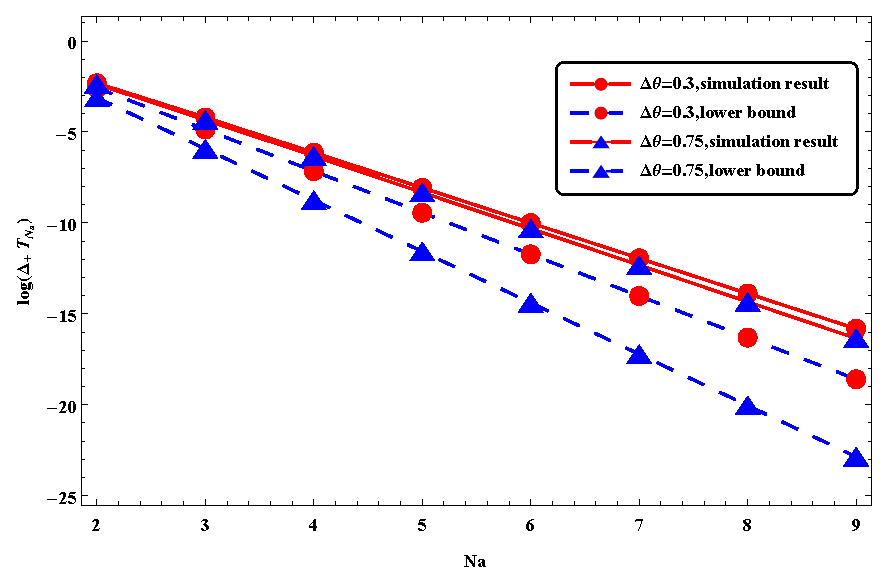
\includegraphics[width=400pt]{decreasing_exponential_lower_bound.eps}
      \caption{连分式指数衰减下界图示}\label{fig:continuous_fraction_exponential_lower_bound}
    \end{figure}

    分析图\ref{fig:continuous_fraction_exponential_lower_bound}可知,对于同等定位强度,如果目标节点角度变化得比较快,则信息衰减得也更快,多条链路后的位置将提供更少的信息量。

%\begin{remark}
%在\ref{section:temporal_cooperative_localization}小节中,我们顺便提到了两个节点时间上一次协作的模型,并在推导得出两个节点时间一%次协作的模型问题可以转化为单节点的模型,但存在一个区别在于这里各时刻速度方向$\theta_i$是随机变量,因此求得的SPEB$\frac{1}%{\lambda}+\frac{1}{T_1}$是关于$\theta_i$的随机变量,要对其求数学期望才能得到平均性能。

%沿用式\ref{eq:recursive_efim}的假设,对诸$\theta_i$求平均后即得平均性能,由于是连分式的形式无法显式给出平均后的结果,但在后续仿真中我%们将分别采用蒙特卡罗模拟的方法估计这个平均性能。

%如果我们考虑的是在固定的时间间隔内加密采样时间,即增大$N_a$,下面的定理指出了$T_1(N_a)$的收敛速度。
%在定理\ref{theorem:arbitrary_curve}的证明过程中已经指出了
%另外由于定理~\ref{theorem:exponential_decreasing}中的信息衰减上下界不含$\theta$,因此也是平均性能提升的衰减速率。如果针对两个节点时%间协作的模型问题,则应
%估计$\sum_{i=N_a}^{2N_a}\frac{1}{q^{2i}}$,结果还是$q^{2N_a}$量级,即$N_a$层后面的所有链路的增益与第$N_a$层的增益相当,即我们有如%下推论,详见附录[\ref{B_F_5}]:
%\end{remark}
%\begin{corollary}[定理\ref{theorem:exponential_decreasing}的推论]\label{corollary:exponential_decreasing}
%在定理\ref{theorem:exponential_decreasing}的的条件下,数列$\{T_{N_a}\}$收敛于$T_{\infty}$,收敛速度是指数收敛的,即\begin{equation}
%\exists q>1,C>0,s.t. |T_{N_a}-T_{\infty}|\leq\frac{C}{q^{N_a}}
%\end{equation}
%\end{corollary}
式(\ref{eq:recursive_efim})的推导过程具有一般性,如果我们不对未知节点测距方差作出相等的假设,也可以得到终点SPEB的连分式表表示形式,推导过程如下:

在$a\bm{I}+b\bm{J}$中提取a,并设$\lambda_{ij}=\frac{b}{a\sigma_{ij}^2}$于是我们只需考虑$\bm{I}+\bm{J}$,其中
\begin{equation}J=\left(
\begin{array}{ccccc}
\lambda_{12}\bm{u}_1\bm{u}_1^{\textrm{T}} &-\lambda_{12}\bm{u}_1\bm{u}_1^{\textrm{T}} &\bm{0}&\dots&\bm{0}\\
&&&&\\
-\lambda_{12}\bm{u}_1\bm{u}_1^{\textrm{T}} &\lambda_{12}\bm{u}_1\bm{u}_1^{\textrm{T}} +&-\lambda_{23}\bm{u}_2\bm{u}_2^{\textrm{T}} &\dots&0\\
&\lambda_{23}\bm{u}_2\bm{u}_2^{\textrm{T}} &&&\\
\vdots &\vdots&\ddots &\vdots&\vdots\\
\bm{0}&\dots&\bm{0}&-\lambda_{N_a-1,N_a}\bm{u}_{N_a-1}\bm{u}_{N_a-1}^{\textrm{T}} &\lambda_{N_a-1,N_a}\bm{u}_{N_a-1}\bm{u}_{N_a-1}^{\textrm{T}} \\
\end{array}
\right).
\end{equation}
类似式~(\ref{eq:recursive_efim}),
我们可以导出终点节点的SPEB$=1+\frac{1}{T_1}$,$T_1$满足下面的递推关系式:
\begin{equation}\label{eq:recursive_efim_second}
  T_i=\frac{1}{\lambda_{i,i+1}^{-1}+\sin^2\theta_i+\frac{\cos^2\theta_i}{T_{i+1}}}
\end{equation}
其基本形式和(\ref{eq:recursive_efim})相同,计算算到$T_{N_a}=1$,
具体推导过程可参考附录[\ref{B_F_3}]

[\ref{B_F_3}]同时证明了,减小诸$\theta$可以提高$T_1$即增大信息量,因此在线性网络中,当目标节点作直线运动时,确定其各个时刻的位置获得的信息量最大,因而精度最高。
\section{正方形网络与正六边形网络}\label{section:square_and_hexagon_network}
在协作定位网络的问题模型下,我们在本节考虑大规模空间协作两种特殊的情形:
正方形网络和正六边形网络。正六边形网络的每个内部节点周围有3个节点与之协作,且该内部节点位于周围三个节点构成的正三角形的重心上。
为研究正六边形网络对定位性能的影响,我们考虑以一个节点$\bm{p}$为网络中心,我们称网络中某节点$\bm{p}_n$位于第n层链路上如果$\bm{p}_n$到$\bm{p}$的最短路径为n,图\ref{HexagonNetwork}就是一个只考虑前两层链路的正六边形网络。
\begin{figure}[h]
  \centering
  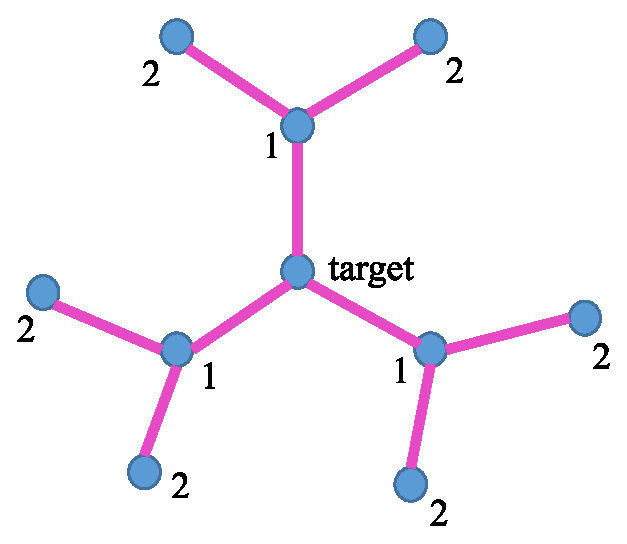
\includegraphics[width=250pt]{massive_spatial.eps}
  \caption{只考虑前两层链路的正六边形网络}\label{HexagonNetwork}
\end{figure}

正方形网络的描述同正六边形网络,如果以目标节点作为坐标原点,含其他未知位置的节点的两条直线作为坐标轴建立平面直角坐标系,
根据前面的正交性的结论,非坐标轴上的点不会对目标节点提供定位信息,而两条坐标轴提供的信息又彼此独立,因此其定位信息量是2个完全相同的部分相加,
每部分由式(\ref{eq:gcf_1})描述,在网络规模很大时近似于极限值$\sqrt{\lambda^2+4\lambda}$。

该结论可以推广至一般矩形网络,且各节点相互测距的方差$\sigma^2_{i,j}$不相等,由式(\ref{eq:recursive_efim_second})可以看出正交性的结论仍然成立,因此非坐标轴上的点不会对目标节点提供定位信息,在实际定位系统的设计中,非坐标轴上的点的信息无需传到目标节点或中央处理器进行解算。

下面我们给出大规模正六边形网络目标节点定位误差界的解析表达式,首先需要下面的引理,推导过程见附录[\ref{B_F_4}]
\begin{lemma}\label{lemma:hexagon}
  设$u$是模长为1的平面向量,那么有:
\begin{equation}\label{eq:equiv}
  u^{\textrm{T}} ((\lambda+\frac{3}{2})I_2-\frac{1}{\lambda+\frac{3}{2}}(\frac{3}{2}I_2-uu^{\textrm{T}} ))^{-1}u
  =((\lambda+\frac{3}{2})-\frac{1/2}{\lambda+\frac{3}{2}})^{-1}.
\end{equation}
\end{lemma}
  由于正六边形网络的特殊性,类似线性网络的情形,我们可以把定位误差下界写出连分式的形式,而上面的引理能够把连分式中与$u$相关的项化为与$u$无关的项,由此推出度为3的协作网络中心节点SPEB满足:
  \begin{equation}
\frac{1}{\text{SPEB}}=\lambda+\frac{3}{2}-\cfrac{3/2}{\lambda+\frac{3}{2}-\cfrac{1/2}{\lambda+3/2-\dots}}.
  \end{equation}
  注意到除了第一层的协作外,后面每层协作由于前一层的削弱系数由3/2变为1/2.
  用同样的方法可求出极限值为:
  \begin{equation}
  \lambda+\frac{3}{2}-\cfrac{3/2}{\lambda+\frac{3}{2}-\cfrac{1/2}{\lambda+3/2-\dots}}=\sqrt{\lambda^2+3\lambda+\frac{1}{4}}-\frac{1}{\lambda+\frac{3}{2}+\sqrt{\lambda^2+3\lambda+\frac{1}{4}}}.
  \end{equation}
  取倒数即为某方向的误差下界,由于网络的各向同性,x方向和y方向的误差下界都是这个数。
且该误差下界总是比正方形网格x或y方向的误差大。

\section{本章小结}\label{section:conclusion4}
  % Keep the summary *very short*.
   本章提供了两种求解定位误差下界的思路:求解特殊矩阵的全部特征值和连分式分析法。

  \begin{itemize}
  \item 求解特殊矩阵的全部特征值能给出高维信息椭圆的全部结构,可以全局地分析误差下界,但已知的能解析求解全部特征值的矩阵非常有限,而且求解本身有很强的技巧性,因此该方法局限性比较大。
  \item 线性网络的费舍尔信息矩阵是块三对角矩阵,块三对角矩阵局部展开后可以得到误差下界的连分式表示法$\ref{eq:U_recursive_formula}$,关于连分式的分析可以相对比较一般,正如 式\ref{eq:recursive_efim_second}所示,我们不需要对线性网络的参数作事先的假定,同时可以通过不等式放缩等技巧对给定的连分式的收敛特性有比较严谨的数学证明。
  \end{itemize}

  同时本章最后借助线性网络中的正交性结论,得到了一般矩形网络中链路信息传播特点,同时还求出了大规模正六边形网络的理论定位误差下界。
\chapter{结论}\label{cha:content5}
    在本文中,我们从协作定位的数学模型出发,通过对费舍尔信息矩阵的分析,研究了定位网络中信息时空传播的机理。首先,我们对费舍尔信息矩阵进行了预处理,将其归为某种类型的矩阵加以研究;同时由于很多时候直接推导存在很大的困难,我们采用猜想-归纳-证明的思路,用数学归纳法给出了部分结论的严谨的证明;
    除此之外,针对推导得出比较复杂的表达式,我们采用了瑞利商、黎曼积分以及连分式等思路进行化简。
    最后,我们结合数值仿真对结论进行了必要的验证。
  \section{已取得的成果}
  % Keep the summary *very short*.
  在数学方法方面,本文主要的成果如下:
  \begin{itemize}
  \item
    使用复数表示法推导得出非协作定位场景下费舍尔信息矩阵的特征值和特征向量的表达式。
  \item
    推导得出秩一矩阵的克罗内克积对N维对称正定矩阵扰动后行列式的表达式。
  \item
    推导得出二维场景下特殊完全图的邻接矩阵所有特征值,其中使用瑞利商给出了最大 特征值的表达式。
  \item 推导得出二维场景下特殊度为2的图的邻接矩阵的所有特征值;当网络规模趋向无穷大时,求出了所有特征值的倒数和的平均值的极限。
  \item 使用连分式推导得出形如式(\ref{eq:Pab})的对称正定矩阵$\bm{A}$确定的$\bm{A}^{-1}_{1\times2,1\times2}$的两个特征值;分析得出了决定特征值的连分式的序列指数收敛的特性,并做出适当的推广。
  \end{itemize}
  \section{工作中的不足之处}
  \begin{itemize}
  \item
  关于两个节点协作的场景中的最优部署角度的结论只是充分性条件,而且结论本身缺少工程直观。
  \item
  考虑的全连接网络过于特殊,而且全连接网络在工程实际中也不现实。
  \item
  关于大规模正方形和正六边形网络的讨论直接给出了结论,由于过程相对很难表述而缺少必要的数学推导或证明。
  \end{itemize}
  \section{未来展望}

  数学方面,本文在线性网络中没有处理成环的情形,环状线性网络对应的费舍尔信息矩阵是循环三对角块状矩阵,应该也可以做出一些好的结果。
  工程方面,本文着重于对网络中信息耦合机理与网络中角度这个几何参量的分析,所研究的模型比较简单,可能与实际问题有一定的出入。今后的工作可以结合计算机仿真工具对复杂网络拓扑下的定位误差作深入的探讨。

%conclusion
%%% 其它部分
\backmatter

%% 本科生要这几个索引,研究生不要。选择性留下。
% 插图索引
\listoffigures
%\listofequations


%% 参考文献
% 注意:至少需要引用一篇参考文献,否则下面两行可能引起编译错误。
% 如果不需要参考文献,请将下面两行删除或注释掉。
\bibliographystyle{thuthesis-numeric}
\bibliography{ref/refs}


%% 致谢
% 如果使用声明扫描页,将可选参数指定为扫描后的 PDF 文件名,例如:
\begin{acknowledgement}[declaration.pdf]
%\begin{acknowledgement}
  衷心感谢导师 沈渊 副教授和数学系 梁恒 副教授对本人的精心指导。他们的言传身教将使我终生受益;感谢黄忠忆教授,本文中关于瑞利商以及部分特殊矩阵特征值的结论即来源于黄老师在课上的讲解。
  同时,我也非常感谢实验室的王云龙师兄、蔡杨师兄,他们在我的毕设期间提供给了我很多宝贵的意见,使我受益匪浅;感谢实验室的刘言师兄,他在我的论文写作过程中就格式规范问题给予了我很多有益的指导;感谢远在千里之外的父母亲时常通过电话给我的鼓励。
  最后感谢 \thuthesis,它的存在让我的论文写作轻松自在了许多,让我的论文格式规整漂亮了许多。
\end{acknowledgement}


%% 附录
\begin{appendix}
%\documentclass[type=bachelor]{thuthesis}
%\documentclass{article}
%\usepackage{xeCJK}%preamble part
%\usepackage{graphicx}
%\usepackage{indentfirst}
%\usepackage{enumerate}
%\usepackage[a4paper, inner=1.5cm, outer=3cm, top=2cm, bottom=3cm, bindingoffset=1cm]{geometry}
%\usepackage{epstopdf}
%\usepackage{listings}
%\usepackage{array}
%\usepackage{fontspec}
%\usepackage{bm}
%\usepackage{gensymb}
%\usepackage{todonotes}
%\usepackage{amsmath, amstheorem, amssymb}
%\usepackage[citecolor=blue]{hyperref}
%\newtheorem{definition}{Definition}
%%\newtheorem{theorem}{Theorem}[section]
%\newtheorem{theorem}{Theorem}
%\newtheorem{corollary}{Corollary}
%\newtheorem{lem}{Lemma}
%\newtheorem{remark}{Remark}
%\DeclareMathOperator{\sgn}{sgn}
%\theoremstyle{remark}
%\newtheorem*{rem}{Remark}
%\setCJKmainfont[BoldFont={SimHei}]{SimSun}
%\setCJKmonofont{SimSun}
%\setmainfont{Times New Roman}
%\newCJKfontfamily[hei]\heiti{SimHei}
%\setlength{\extrarowheight}{4pt}
%\setlength{\parindent}{1cm}
%
%\pagenumbering{arabic} 
%\begin{document}
%\setcounter{page}{40}
%\title{协作定位中的信息耦合} 
%\author{\fontsize{12pt}{\baselineskip}{沈渊,清华大学电子工程系副教授}}
%\maketitle
%\begin{appendix}
\chapter{外文资料的调研阅读报告或书面翻译}
\title{第一篇--协作定位中的信息耦合$^{[1]}$}
\textbf{摘要}:
%第一篇论文翻译,原文的题目是
%Information Coupling in Cooperative Localization
%,原文的摘要翻译如下:
不依赖环境的高精度协作定位网络能有一系列的重要的应用。但是现有的分布式协作定位算法没有考虑到预测节点位置彼此之间的相关性。这篇文章通过费舍尔信息量的度量研究了协作定位网络的相关性问题,产生了信息耦合这个概念。为了描述这个特性,我们重点关注了最简单的非平凡情形并且推导出了信息耦合的表达式。
\section{符号约定}
$\text{tr}{\bm{A}},\text{adj}{\bm{A}}$和$
|\bm{A}|$分布表示方阵A的迹,伴随矩阵和行列式。
$[\cdot]^T$表示变量的转置;$\mathbb{S}^2,\mathbb{S}^2_+,\mathbb{S}^2_{++}$分别表示$2\times 2$的实矩阵、半正定矩阵和正定矩阵。另外$\angle \{ \bm{u},\bm{v}\}
$表示向量$\bm{u}$和向量$\bm{v}$之间的夹角。
\section{协作定位中的联合估计}
考虑一个有$\mathcal{N}_a$个移动节点和$\mathcal{N}_b$个移动节点的协作定位网络,锚点的位置已知${\bm{p}_j:j \in \mathcal{N}_b}$,并且移动节点尝试通过和邻居节点的测距和通信确定它们自己的位置${\bm{p}_k: k \in \mathcal{N}_a}$。
在文献[2]确定的测距信息是FIM的基本组成模块,这种测距信息描述了关于从测量中获得的距离信息的强度和方向。
\begin{definition}
在节点k和j之间的总的测距信息强度(RII)定义为关于从它们之间的距离测量中得到的距离$d_{k,j}=||\bm{p}_k-\bm{p}_j||$的费舍尔信息量。
\end{definition}
\begin{definition}
设$\bm{u}_{i_1,i_2}$为从节点$i_1$到节点$i_2$的单位方向向量。定义$\bm{C}^{n,m}_{k,j}$是关于$k,j,n,m \in \mathcal{N}_a \cup \mathcal{N}_b$矩阵:
\[
\bm{C}^{n,m}_{k,j} \triangleq \frac{\bm{u}_{k,j}\bm{u}_{n,m}^T+\bm{u}_{n,m}\bm{u}_{k,j}^T}{2} \in \mathbb{S}^2
\]
另外,定义
\[
\mathring{\bm{C}}^{n,m}_{k,j} \triangleq \frac{\mathring{\bm{u}}_{k,j}\mathring{\bm{u}}_{n,m}^T+\mathring{\bm{u}}_{n,m}\mathring{\bm{u}}_{k,j}^T}{2} \in \mathbb{S}^2
\]
\end{definition}

其中$\mathring{\bm{u}}_{i_1,i_2}$为逆时针方向上垂直于$\bm{u}_{i_1,i_2}$的单位向量,另外,为记号上的简便,$\bm{C}_{k,j}=\bm{C}^{k,j}_{k,j} \in \mathbb{S}^2_+$。
EFIM的概念[6]让我们能直接通过Schur补的方法从FIM中推导对于参数向量的一个子集的信息不等式。由于在已知移动节点位置的条件下测距彼此之间相互独立,对于移动节点位置的EFIM可以写成闭式解的形式。用求导的链式法则可以证明,对于协作定位这种EFIM是下面分块矩阵的形式:
\begin{equation}\label{eq:FIM}
\bm{J}_e=\left[\begin{array}{cccc}
\bm{K}_1^{\mathcal{N}_a \backslash \{1\}} & -\zeta_{1,2} \bm{C}_{1,2} &\cdots & -\zeta_{1,N_a} \bm{C}_{1,N_a} \\
-\zeta_{1,2} \bm{C}_{1,2} &\bm{K}_2^{\mathcal{N}_a \backslash \{2\}} & \cdots & -\zeta_{2,N_a} \bm{C}_{2,N_a} \\
\vdots & \vdots & \ddots & \vdots\\
-\zeta_{1,N_a} \bm{C}_{1,N_a} & -\zeta_{2,N_a} \bm{C}_{2,N_a} & \cdots & \bm{K}_2^{\mathcal{N}_a \backslash \{N_a\}}\\
\end{array}
\right]
\end{equation}
其中$\mathcal{N}_a=\{1,2 \dotsc N_a\}$,对于$k,j \in \mathcal{N}_a,\zeta_{k,j}$是节点k和节点j总的RII,并且
\[
\bm{K}^{\mathcal{N}}_k=\bm{J}^{\mathcal{N}_b}_k+\sum_{j\in \mathcal{N}} \zeta_{k,j} \bm{C}_{k,j}, \mathcal{N} \subset \mathcal{N}_a
\]
上式中$\bm{J}^{\mathcal{N}_b}_k$表示仅从和$\mathcal{N}_b$测距中获得的关于第k个节点的EFIM。
\begin{remark}
对于式(\ref{eq:FIM})中表示协作定位的EFIM不是对角矩阵,反映了从达到CRLB的位置估计量推断中的移动节点间位置信息是相关的。这种情况阻碍了针对协作定位的最优或次优的分布式算法的设计。%development->设计?
因此在接下来的分析中我们会探究由于非对角结构引起的信息耦合的表现。
\end{remark}
\section{信息耦合}
为获得信息耦合的洞见,我们考虑一个含有$\mathcal{N}_b$个移动节点和三个协作节点的网络:$\mathcal{N}_a=\{1,2,3\}$,这代表了一个最简单的非平凡的信息耦合的情形。下面我们推导每一个移动节点的EFIM和它的逆的闭式解。
\begin{definition}
给定$\zeta_{k,j} \in (0,\infty)$和$\bm{J} \in \mathbb{S}^2_{++}$。定义$\Phi_{k,j}(\bm{J})$是如下形式的商:
\[
\Phi_{k,j}(\bm{J})\triangleq=\frac{|\bm{J}|}{|\bm{J}+\zeta_{k,j}\bm{C}_{k,j}|}\in (0,1).
\]
\end{definition}
\begin{remark}
注意到$\forall \bm{J} \in \mathcal{S}^2_{++},\lim_{\zeta_{k,j} \rightarrow 0}\Phi_{k,j}=1$并且$\lim_{\zeta_{k,j} \rightarrow \infty}\Phi_{k,j}=0$.此外,$\forall \zeta_{k,j} \in (0,\infty)$,$\lim_{|\bm{J}|\rightarrow 0}\Phi_{k,j}=0$并且$\lim_{|\bm{J}|\rightarrow \infty}\Phi_{k,j}=1.$又因为$|\bm{J}+\zeta_{k,j}|=|\bm{J}|+\zeta_{k,j}\bm{u}_{k,j}\text{adj}\{\bm{J}\}\bm{u}_{k,j},$
\[
\frac{\mu_2}{\mu_2+\zeta_{k,j}}\leq \Phi_{k,j}(\bm{J})\leq \frac{\mu_1}{\mu_1+\zeta_{k,j}}
\]
其中 $\mu_1 \geq \mu_2 \ge 0$是$\bm{J}$的两个特征根。$\Phi_{k,j}(\bm{J})$表示从节点j获得的$\zeta_{k,j}$(RII)中可以被节点k有效利用的部分,而$\bm{J}$是这个部分中的不确定性。
\end{remark}
\begin{theorem}
设$\bm{J}_1^{\mathcal{N}_b},\bm{J}_2^{\mathcal{N}_b},\bm{J}_3^{\mathcal{N}_b}$分别表示仅从锚点$\mathcal{N}_b$获得的EFIM,则移动节点1的EFIM由下式给出:
\begin{equation}
\bm{J}_1=\bm{J}_1^{\mathcal{N}_b}+\check{\zeta}_{1,2}\bm{C}_{1,2}+\check{\zeta}_{1,3}\bm{C}_{1,3}+\kappa_{2,3}\bm{C}^{1,3}_{1,2}
\end{equation}
其中
\begin{eqnarray}
\check{\zeta}_{1,2}&=\zeta_{1,2} \cdot \Phi_{1,2}(\bm{J}_2^{\mathcal{N}_b}+\zeta_{2,3} \cdot \Phi_{2,3}(\bm{K}_3^{1})\cdot \bm{C}_{2,3})\\
\check{\zeta}_{1,3}&=\zeta_{1,3} \cdot \Phi_{1,3}(\bm{J}_3^{\mathcal{N}_b}+\zeta_{2,3} \cdot \Phi_{2,3}(\bm{K}_2^{1})\cdot \bm{C}_{2,3})
\end{eqnarray}
并且$\kappa_{2,3}$由(5)式给出。
此外,EFIM的逆为:
\begin{equation}
\bm{J}^{-1}=\frac{1}{|\bm{J}_1|}[\text{adj}\{\bm{J}^{\mathcal{N}_b}_1\}+\check{\zeta}_{1,2}\mathring{\bm{C}}_{1,2}+\check{\zeta}_{1,3}\mathring{\bm{C}}_{1,3}+\kappa_{2,3}\mathring{\bm{C}}_{1,2}^{1,3}]
\end{equation}
其中$|\bm{J}_1|$由(7)式给出。
\end{theorem}
\begin{remark}
移动节点1的EFIM和它的逆都是三项的和,分别对应着从锚点、协作获取的信息以及耦合项。特别的,在(2)式中,第一项$\bm{J}_1^{\mathcal{N}_b}$是从锚点获取的信息,第二项$\check{\zeta}_{1,2}\bm{C}_{1,2}+\check{\zeta}_{1,3}\bm{C}_{1,3}$是从节点12连线和节点13连线获得的信息增量,这个增量取决于RII和由(3)式和(4)式给出的协作节点位置的不确定性。第三项$\kappa_{2,3}\bm{C}_{1,2}^{1,3}$是来自节点2和3的信息耦合项,这一项的的出现是由于节点2和3彼此之间也有协作。在描述EFIM的逆的(6)式中,三项共同的伸缩因子是行列式$|\bm{J}_1|$的倒数,并且后面的每个矩阵都是由原来的单位向量逆时针转90度再做外积得到的。
\end{remark}
从(5)式可以得到,$\kappa_{2,3}$的一个上界是:
\[
\kappa_{2,3}\leq 2\zeta_{1,2}\zeta_{1,3}\zeta_{2,3}|\bm{u}_{1,2}^T(\bm{J}_2^{\mathcal{N}_b})^{-1}\bm{C}_{2,3}(\bm{J}_3^{\mathcal{N}_b})^{-1}\bm{u}_{1,3}|
\]
从上式可以看出,在如下情形中没有耦合:
\begin{enumerate}[(i)]
\item{如果$\angle \{\bm{u}_{1,2},\bm{J}_2^{\mathcal{N}_b}\bm{u}_{2,3}\}$或者$\angle \{\bm{u}_{1,3},\bm{J}_3^{\mathcal{N}_b}\bm{u}_{2,3}\}$为90度,那么$\kappa_{2,3}=0$;}
\item{如果移动节点2成为一个锚点,也就是$|\bm{J}_2^{\mathcal{N}_b}|$趋向于无穷大,那么$\check{\zeta_{1,2}}=\zeta_{1,2},\check{\zeta_{1,3}}=\zeta_{1,3}\cdot \Phi_{1,3}(\bm{J}_3^{\mathcal{N}_b}+\zeta_{2,3}\bm{C}_{2,3}),$并且$\kappa_{2,3}=0$;}
\item{如果节点2和节点3之间不协作,也就是$\zeta_{2,3}=0$,那么$\check{\zeta_{1,2}}=\zeta_{1,2}\cdot \Phi_{1,2}(\bm{J}_2^{\mathcal{N}_b},\check{\zeta_{1,3}}=\zeta_{1,3}\cdot \Phi_{1,3}(\bm{J}_3^{\mathcal{N}_b}),$并且$\kappa_{2,3}=0$;}
\end{enumerate}
这些结果说明了当移动节点的位置满足(i)中的正交性条件或者如$(ii)$或$(iii)$给出的有少于3个节点参与协作时,不会有耦合项出现。
\begin{corollary}
耦合项$\kappa_{2,3}\bm{C}_{1,2}^{1,3}$有特征值$[\cos(\angle \{\bm{u}_{1,2},\bm{u}_{1,3}\})+1]\kappa_{2,3}/2$和$[\cos(\angle \{\bm{u}_{1,2},\bm{u}_{1,3}\})-1]\kappa_{2,3}/2$,分别对应的特征向量是$
\bm{u}_{1,2}+\bm{u}_{1,3}$和$\bm{u}_{1,2}-\bm{u}_{1,3}$。
\end{corollary}
\begin{remark}
这个引理说明了如果$\kappa_{2,3}>0$(对应的,如果$\kappa_{2,3}<0$),如果忽略耦合项,由协作获得的信息椭圆在$
\bm{u}_{1,2}+\bm{u}_{1,3}$方向上会被低估(对应的,高估),而在$
\bm{u}_{1,2}-\bm{u}_{1,3}$方向上会被高估(对应的,低估)。另外当角$\angle \{\bm{u}_{1,2},\bm{u}_{1,3}\}$是锐角(对应的,钝角)时,在$
\bm{u}_{1,2}+\bm{u}_{1,3}$方向上的信息耦合会比$
\bm{u}_{1,2}-\bm{u}_{1,3}$方向上的更显著(对应的,不如前者显著)。
\end{remark}
\begin{figure}
\centering
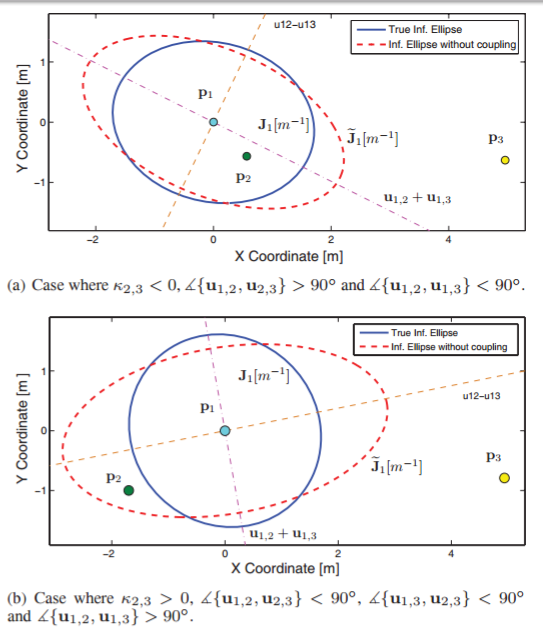
\includegraphics[width=\textwidth/2]{figure_2.png}
\caption{协作定位中的信息耦合可能会严重实际可达到的定位信息}
\end{figure}

举例说明如下,图1描述了考虑和忽略耦合项的信息椭圆的形状。在这两种类别中,从锚点获得的EFIM为简便取成$\bm{J}^{\mathcal{N}_b}_1,\bm{J}^{\mathcal{N}_b}_2,\bm{J}^{\mathcal{N}_b}_3=\text{diag}\{1,1\}$,并且三个协作节点分别位于位置$\bm{p}_1,\bm{p}_2,\bm{p}_3$.
图1展示了节点1的真实信息椭圆$\bm{J}_1$和忽略耦合项后的信息椭圆$\bm{\tilde{J}}_1$的差别。
%\newpage
%% \documentclass[10pt,journal,compsoc]{IEEEtran}
% \usepackage{xeCJK}%preamble part
% \usepackage{graphicx}
% \usepackage{pdfpages}
% \usepackage{indentfirst}
% \usepackage{enumerate}
% \usepackage[a4paper, inner=1.5cm, outer=3cm, top=2cm, bottom=3cm, bindingoffset=1cm]{geometry}
% \usepackage{epstopdf}
% \usepackage{listings}
% \usepackage{array}
% \usepackage{fontspec}
% \usepackage{bm}
% \usepackage{gensymb}
% \usepackage{todonotes}
% \usepackage{amsmath, amsthm, amssymb}
% \usepackage[citecolor=blue]{hyperref}
% \newtheorem{definition}{Definition}
%\newtheorem{thm}{Theorem}[section]
% \newtheorem{thm}{Theorem}
% \newtheorem{corollary}{Corollary}
% \newtheorem{lem}{Lemma}
% \newtheorem{remark}{Remark}
% \newtheorem{proposition}{Proposition}
% \DeclareMathOperator{\sgn}{sgn}
% \theoremstyle{remark}
% \newtheorem*{rem}{Remark}
% \setCJKmainfont[BoldFont={SimHei}]{SimSun}
% \setCJKmonofont{SimSun}
% \setmainfont{Times New Roman}
% \newCJKfontfamily[hei]\heiti{SimHei}
% \setlength{\extrarowheight}{4pt}
% \setlength{\parindent}{1cm}
 
%\begin{document}
\title{第二篇--协作定位网络中的时空信息耦合$^{[2]}$} 
%\author{\fontsize{12pt}{\baselineskip}{沈渊,清华大学电子工程系副教授}}
%\markboth{Journal of \LaTeX\ Class Files,~Vol.~14, No.~8, August~2015}%
%{Shell \MakeLowercase{\textit{et al.}}: Bare Advanced Demo of IEEEtran.cls for IEEE Computer Society Journals}
%\IEEEtitleabstractindextext{
%\begin{abstract}
\textbf{摘要}:%第二篇论文翻译,原文的题目是
%Spatio-Temporal Information Coupling in Cooperative Network Navigation
%原文的摘要翻译如下:
可靠的定位信息对很多基于位置的应用起着至关重要的作用。通过时空联合协作的网络导航可以给移动节点提供高精度和鲁棒的位置信息。同时,由于待测节点的位置相关,这种联合协作导致了错综复杂的信息获取方式,也就是信息耦合的问题。在这篇文章中,通过对费舍尔信息量的分析,我们在四种有代表性的情形中量化了信息耦合。我们说明了每个节点所获得的信息来自与它进行时空协作的节点和由于和邻居节点的协作产生的信息耦合。我们的结果为网络中复杂信息获取提供了洞见,并且能够为高效的网络导航算法提供指导。
%\end{abstract}
%}\maketitle
%reset section counter here
\setcounter{section}{0}
\section{简介}
关于研究背景的翻译略去,下面是原文一些记号上的约定。
$[\cdot]^T$表示变量的转置;$\mathbb{S}^D,\mathbb{S}^D_+,\mathbb{S}^D_{++}$分别表示$D\times D$的实矩阵、半正定矩阵和正定矩阵。$\bm{J}_r(\bm{v}):=\bm{v}\bm{v}^T$表示由向量$\bm{v}$做外积得到的秩1阵。
另外$\angle \{ \bm{u},\bm{v}\}
$表示向量$\bm{u}$和向量$\bm{v}$之间的夹角。
\section{网络导航中的费舍尔信息量}
在本节中,我们首先介绍网络模型和网络导航中的FIM作为预备知识,然后描述这篇文章重点讨论的4种场景。
\subsection{预备知识}
考虑一个由若干节点构成的协作网络,用$\bm{x}_k^{(n)}\in \mathbb{R}^D$表示节点k在时间$t_n$的位置状态,$k=1,2,....,N$且$n=1,2,...T$.网络导航的目标是从测量和先验信息中推断节点的位置信息。
令$\mathcal{S}=\{1,2,...,S\}\text{ with }S=N\cdot T$是位置状态的下标集,文献[8]已经证明了对于S个位置状态FIM可以分解成:
\begin{equation}
\bm{J}=\sum_{(i,j)\in \mathcal{S}^2,i\geq j} \bm{G}^S_{i,j} \otimes \bm{K}_{i,j}
\end{equation}
其中$\otimes$表示Kronecker矩阵积,$S\times S$的矩阵$\bm{G}^S_{i,j}$的元素$(k,r)$由下式给出:
\[
[\bm{G}^S_{i,j}]_{k,r}=\left\{
\begin{array}{c l}	
     1 & k=r=i\\
     1 & k=r=j\\
     -1 & k=i,r=j,k \neq r\\
     -1 & k=j,r=i,k \neq r\\
     0, & \text{otherwise}
\end{array}\right.
\]
$\bm{K}_{i,j}\in \mathbb{S}_+^D$ 描述了包含在测量或先验知识中和位置状态i,j有关的位置信息。$\bm{K}_{i,j}=\bm{K}_{j,i}$并且在缺少关于位置状态i,j的测量或先验知识的情况下$\bm{K}_{i,j}=0$。特别的,如果$i=j$,$\bm{K}_{i,i}$描述了仅仅和位置状态i有关的位置信息。
\subsection{有代表性的场景}
我们考虑图1中的四种场景以获得对时空协作的洞见。
\begin{figure}
\centering
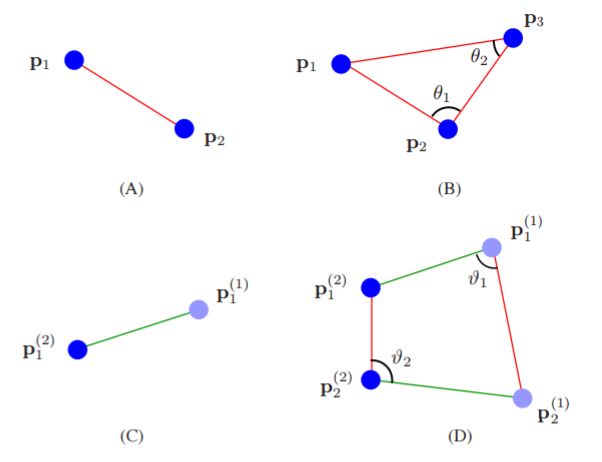
\includegraphics[width=\textwidth/2]{figure_1.png}
\caption{四种场景:(A)两个节点的空间协作(红色的连接);(B)三个节点的空间协作;(C)一个节点的时间协作(绿色的连接);(D)两个节点的时空协作。}
\end{figure}

在这些场景中,位置状态就是节点的位置,节点通过和位置已知的锚点和位置未知的邻居节点的测距中获得位置信息。
在接下来的讨论中,在时间步为n时,$\bm{K}^{(n)}_{i,i}$表示节点i从锚点获取的信息;$\bm{u}_{i,j}^{(n)}$表示节点i和j连线的单位方向向量;$\lambda^{(n)}_{i,j}=\lambda^{(n)}_{j,i}$表示节点i和j之间的测距信息强度(RII);$\bm{u}_{i,i}^{(n)}$表示链接节点i在时间步为n和n+1时的位置的单位方向向量;$\lambda^{(n)}_{i,i}$表示节点i的速度信息强度(SII)。

\textbf{场景A:}两个节点通过彼此测距协作来确定它们的位置,即位置状态是$\bm{p}_1$和$\bm{p}_2$,测距信息是$\bm{J}_r(\bm{v}_{1,2})$,其中$\bm{v}_{1,2}=\sqrt{\lambda_{1,2}}\bm{u}_{1,2}$,因此,基于(1)式我们得到这种场景的FIM是:
\begin{equation}
\bm{J}_A=\left[
\begin{array}{cc}
\bm{K}_{1,1}+\bm{J}_r(\bm{v}_{1,2})&-\bm{J}_r(\bm{v}_{1,2})\\
-\bm{J}_r(\bm{v}_{1,2})&\bm{K}_{2,2}+\bm{J}_r(\bm{v}_{1,2})\\
\end{array}
\right]
\end{equation}
%\begin{figure*}[!t]
\begin{equation*}
\bm{J}_B=\left[
\begin{array}{ccc}
\bm{K}_{1,1}+\bm{J}_r(\bm{v}_{1,2})+\bm{J}_r(\bm{v}_{1,2}) & -\bm{J}_r(\bm{v}_{1,2}) & -\bm{J}_r(\bm{v}_{1,3})\\
-\bm{J}_r(\bm{v}_{1,2}) &\bm{K}_{2,2}+\bm{J}_r(\bm{v}_{1,2})+\bm{J}_r(\bm{v}_{2,3}) & -\bm{J}_r(\bm{v}_{2,3})\\
 -\bm{J}_r(\bm{v}_{1,3}) & -\bm{J}_r(\bm{v}_{2,3})&
\bm{K}_{3,3}+\bm{J}_r(\bm{v}_{1,3})+\bm{J}_r(\bm{v}_{2,3})\\
\end{array}
\right]
\end{equation*}
%\hrulefill
%\vspace*{4pt}
%\end{figure*}

\textbf{场景B:} 三个节点通过彼此测距协作确定它们的位置,即位置状态是$\bm{p}_1,\bm{p}_2$和$\bm{p}_3$,测距信息是$\bm{J}_r(\bm{v}_{i,j})$对于$i,j\in \{1,2,3\},i\neq j$,其中$\bm{v}_{i,j}=\sqrt{\lambda_{i,j}}\bm{u}_{i,j}$,因此,基于式(1)我们可以得到这种情形的FIM由(3)给出,在下一页的最开始的地方。

\textbf{场景C:}单节点在两个不同的时刻通过速度测量协作来确定自身的位置,即位置状态是$\bm{p}^{(1)}_1$和$\bm{p}^{(2)}_1$,速度测量的信息是$\bm{J}_r(\bm{t})$,其中$\bm{t}=\sqrt{\lambda^{(1)}_{1,1}}\bm{u}_{1,1}^{(1)}$.因此基于(1),我们得到这种场景的FIM是:
\[\bm{J}_C=\left[
\begin{array}{cc}
\bm{K}_{1,1}^{(1)}+\bm{J}_r(\bm{t})&-\bm{J}_r(\bm{t})\\
-\bm{J}_r(\bm{t})&\bm{K}_{2,2}^{(2)}+\bm{J}_r(\bm{t})\\
\end{array}\right]
\]

\textbf{场景D:}两个节点在两个不同的时刻协作来确定它们的位置,即,位置状态是$\bm{p}_1^{(1)},\bm{p}_2^{(1)},\bm{p}_1^{(2)}$和$\bm{p}_2^{(2)}$,每个节点测量自身的速度和相对另一节点的距离,并且
\begin{itemize}  
\item 测距信息是$\bm{J}_r(\bm{v}_{1,2})$和$\bm{J}_r(\bm{w}_{i,j})$,其中$\bm{v}_{1,2}=\sqrt{\lambda_{1,2}^{(1)}}\bm{u}^{(2)}_{1,2}$,而$\bm{w}_{1,2}=\sqrt{\lambda_{1,2}^{(2)}}\bm{u}^{(1)}_{1,2}$
\item 测速信息是$\bm{J}_r(\bm{t}_1)$和$\bm{J}_r(\bm{t}_2)$,其中$\bm{t}_i=\sqrt{\lambda_{i,i}^{(1)}}\bm{u}^{(1)}_{i,i}$
\end{itemize}
因此,基于(1)式我们得到这种类形的FIM是
\[
\bm{J}_D=\left[
\begin{array}{cc}
\bm{J}^{(1)}_A+\bm{T}&-\bm{T}\\
-\bm{T}&\bm{J}^{(2)}_A+\bm{T}\\
\end{array}
\right]
\]
其中$\bm{J}^{(1)}_A$和$\bm{J}^{(2)}_A$由(2)式给出,上标代表了时间步长,$\bm{T}=\text{diag}\{\bm{J}_r(\bm{t}_1),\bm{J}_r(\bm{t}_2)\}$.
\section{空间信息耦合}
在这一节中,我们推导了场景A和场景B的EFIM,并且描述了场景B中由于空间协作导致的信息耦合。由于篇幅所限,这篇文章的大部分证明略去。
\begin{proposition}
场景A中节点1的EFI是
\[
\bm{J}_e=\bm{K}_{1,1}+(1-\mu_2^{1,1})\bm{J}_r(\bm{v}_{1,2})
\]
其中
\begin{eqnarray*}
\mu_2^{1,1}=&\bm{v}^T_{1,2}(\bm{K}_{2,2}+\bm{J}_r(\bm{v}_{1,2}))^{-1}\bm{v}_{1,2}\\
=&1-(1+\lambda_{1,2}\bm{u}^T_{1,2}\bm{K}^{-1}_{2,2}\bm{u}_{1,2})^{-1}.
\end{eqnarray*}
此外,$\bm{J}_e \preceq \bm{K}_{1,1}+\bm{J}_r(\bm{v}_{1,2}).$
\end{proposition}
\begin{remark}
场景A中节点1的EFIM是来自锚点和来自与节点2的协作的信息之和。协作在与节点2的连线方向上增加了信息,而节点1可以有效利用的RII随RII $\lambda_{1,2}$增大而增大而随节点2位置在$\bm{u}_{1,2}$方向的不确定性(即$\bm{u}^T\bm{K}^{-1}_{2,2}\bm{u}_{1,2}$)的增大而减小。此外,有效RII总是小于或等于RII。当锚点在节点1,2连线方向上给节点2提供无穷大的信息量时取等号,而当锚点
在这一方向上不提供任何信息时取0。
\end{remark}
\begin{proposition}
在场景B中节点1的EFIM是
\begin{equation}
\begin{split}
\bm{J}_e=\bm{K}_{1,1}+(1-\mu_2^{1,1})\bm{J}_r(\bm{v}_{1,2})+(1-\mu_3^{1,1})\bm{J}_r(\bm{v}_{1,3})\\
+\delta\bm{J}_r(\mu_2^{1,3}\bm{v}_{1,2}+\mu_3^{1,2}\bm{v}_{1,3})
\end{split}
\end{equation}
其中$\mu_i^{j,k}=\bm{v}^T_{j,i}(\bm{K}_{i,i}+\bm{J}_r(\bm{v}_{1,i}))^{-1}\bm{v}_{k,i}$,并且$\delta=(1+\mu_2^{3,3}+\mu_3^{2,2})^{-1}$.除此之外,$\bm{J}_e \preceq \bm{K}_{1,1}+\bm{J}_r(\bm{v}_{1,2})+\bm{J}_r(\bm{v}_{1,3})$.
\end{proposition}
\begin{remark}
命题2说明了场景B下节点1的EFIM是4项的和。第一项对应着从锚点获取的信息,其他三项对应着由于空间协作获得的信息。第二项和第三项对应着沿着与节点2和节点3的连线方向获取的有效信息,而最后一项代表着由于节点2和3协作造成的信息耦合。最后一项是一个秩一阵,有一个非负的特征值$\delta ||\mu_2^{1,3}\bm{v}_{1,2}+\mu_3^{1,2}\bm{v}_{1,3}||^2$并且这个特征值对应的特征向量是$\mu_2^{1,3}\bm{v}_{1,2}+\mu_3^{1,2}\bm{v}_{1,3}$,这个方向既依赖于RII,又依赖于节点2和3位置的不确定性,还和节点的空间拓扑有关。
\end{remark}
接下来我们将说明节点2和3的协作强度如何影响节点1的EFIM.
\begin{corollary}
设$\lambda_{2,3}$和$\tilde{\lambda}_{2,3}$分别表示节点2和节点3之间两个RII,并且$(\mu_2^{1,3},\mu_3^{1,2},\delta),(\tilde{\mu}_2^{1,3},\tilde{\mu}_3^{1,2},\tilde{\delta})$分别表示命题2中对应的两组参数,而其他参数均相同。那么:
\begin{equation}
\delta \bm{J}_r(\mu_2^{1,3}\bm{v}_{1,2}+\mu_3^{1,2}\bm{v}_{1,3}) \preceq \tilde{\delta} \bm{J}_r(\tilde{\mu}_2^{1,3}\bm{v}_{1,2}+\tilde{\mu}_3^{1,2}\bm{v}_{1,3})
\end{equation}
当且仅当$\lambda_{2,3}\leq \tilde{\lambda}_{2,3}$。此外
\[
\lim_{\lambda_{2,3} \rightarrow \infty}\delta \bm{J}_r(\mu_2^{1,3}\bm{v}_{1,2}+\mu_3^{1,2}\bm{v}_{1,3})=\bar{\delta} \bm{J}_r(\bar{\mu}_2^{1,3}\bm{v}_{1,2}+\bar{\mu}_3^{1,2}\bm{v}_{1,3})
\]
其中
\[
\bar{\mu}_2^{1,3}=\bm{v}_{1,2}^T(\bm{K}_{2,2}+\bm{J}_r(\bm{v}_{1,2}))^{-1}\bm{u}_{2,3}
\]
\[
\bar{\mu}_3^{1,2}=\bm{v}_{1,3}^T(\bm{K}_{3,3}+\bm{J}_r(\bm{v}_{1,3}))^{-1}\bm{u}_{2,3}
\]
\[
\bar{\delta}=(\bm{u}_{2,3}^T((\bm{K}_{2,2}+\bm{J}_r(\bm{v}_{1,2}))^{-1}+(\bm{K}_{3,3}+\bm{J}_r(\bm{v}_{1,3}))^{-1})\bm{u}_{2,3})^{-1}.
\]
\end{corollary}
\begin{remark}
从(5)中可以知道,当节点2,3方向保持不变时,节点1从和节点2和3协作中获得的信息随着节点2和3之间的RII的增大而增大。另外,这个信息量的上界是在节点2和3之间测距是理想情况时取得。
\end{remark}
在下面这个推论中,我们将说明如果从协作中获得的信息是分别和节点2,节点3的测距信息的加权和这种情形。
\begin{corollary}
场景B中节点1的EFIM可以写成
\[
\bm{J}_e=\bm{K}_{1,1}+\eta_1 \bm{J}_r(\bm{v}_{1,2})+\eta_2 \bm{J}_r(\bm{v}_{1,3}),\eta_1,\eta_2 \geq 0
\]
当且仅当至少下面至少有一个条件满足:
\begin{itemize}
\item{三个节点共线}
\item $\lambda_{1,2}\cdot \lambda_{1,3}\cdot \lambda_{2,3}=0$
\item $\bm{u}_{1,2}^T(\bm{K}_{2,2}+\bm{J}_r(\bm(v)_{1,2}))^{-1}\bm{u}_{2,3}=0$
\item $\bm{u}_{1,3}^T(\bm{K}_{3,3}+\bm{J}_r(\bm(v)_{1,3}))^{-1}\bm{u}_{2,3}=0$
\end{itemize}
\end{corollary}
接下来我们将说明如果锚点提供各向同性的信息给节点2,3,那么权重参数$\mu_i^{j,k}$可以写成$\theta_1=\angle \{\bm{u}_{1,2},\bm{u}_{2,3}\}$和$\theta_2=\angle \{\bm{u}_{1,3},\bm{u}_{2,3}\}$的函数。
\begin{corollary}
如果$\bm{K}_{i,i}=\xi_i\bm{I}$对于$i=2,3$成立,则场景B中节点1的EFIM为
\begin{equation*}
\begin{split}
\bm{J}_e=\bm{K}_{1,1}+\frac{\xi_2}{\xi_2+\lambda_{1,2}}\bm{J}_r(\bm{v}_{1,2})+\frac{\xi_3}{\xi_3+\lambda_{1,3}}\bm{J}_r(\bm{v}_{1,3})\\
+\delta\bm{J}_r(\mu_2^{1,3}\bm{v}_{1,2}+\mu_3^{1,2}\bm{v}_{1,3})
\end{split}
\end{equation*}
其中
\[
\mu_2^{1,3}=\frac{\sqrt{\lambda_{1,2}\lambda_{2,3}}\cos \theta_1}{\xi_2+\lambda_{1,2}}
\]
\[
\mu_3^{1,2}=\frac{\sqrt{\lambda_{1,3}\lambda_{2,3}}\cos \theta_2}{\xi_3+\lambda_{1,3}}
\]
\[
\mu_2^{3,3}=\frac{\lambda_{2,3}}{\xi_2}(1-\frac{\lambda_{1,2}\cos^2 (\theta_2)}{\xi_2+\lambda_{1,2}})
\]
\[
\mu_3^{2,2}=\frac{\lambda_{2,3}}{\xi_3}(1-\frac{\lambda_{1,3}\cos^2 (\theta_2)}{\xi_3+\lambda_{1,3}})
\]
\end{corollary}
\begin{remark}
这个结果说明了如果$(i)$节点2和3来自锚点或先验的信息是各向同性的$(ii)\bm{u}_{1,2}\perp\bm{u}_{2,3}$或者$\bm{u}_{1,3}\perp\bm{u}_{2,3}$,那么节点1通过写作获得的信息是分别来自节点2的测距信息的加权和。
\end{remark}
\section{空时信息耦合}
在本节中,我们推导出了场景C和D下节点1在时间步2时的EFIM,并且描述了场景D中由于空时协作产生的信息耦合。
\begin{proposition}
场景C中节点1的EFIM是
\[
\bm{J}_e=\bm{K}_{1,1}^{(2)}+\frac{\lambda_{1,1}^{(1)}}{1+\lambda_{1,1}^{(1)}\bm{u}_{1,1}^T(\bm{K}_{1,1}^{1})^{-1}\bm{u}_{1,1}}\bm{J}_r(\bm{u}_{1,1})
\]
此外$\bm{J}_e \preceq \bm{K}_{1,1}^{(2)}+\bm{J}_r(\bm{t})$.
\end{proposition}
\begin{remark}
与场景A类似,场景C中时间步为2时节点1的EFIM是从锚点获取的信息和与节点1在时间步为1时的协作信息之和。协作在节点1在两个时刻位置连线的方向上增加了信息,而节点1可以有效利用的SII随SII $\lambda_{1,1}^{(1)}$的增加而增大而随着节点1在时间步1的位置不确定性(即方向$\bm{u}_{1,1}^T(\bm{K}_{1,1}^{(1)})^{-1}\bm{u}_{1,1}$)的增大而减小。此外,有效的SII总是小于等于SII,当锚点给时间步1时的节点提供无穷大的信息时取等号,当不提供任何信息时取0.
\end{remark}
\begin{proposition}
场景D中节点1在时间步2时的EFIM是
\begin{equation}
\begin{split}
\bm{J}_e=\bm{K}_{1,1}^{(2)}+&[1-\bm{v}_{1,2}^T(\bm{K}_{2,2}^{(2)}+\bm{H}_{1,2})^{-1}\bm{v}_{1,2}]\bm{J}_r(\bm{v}_{1,2})\\
+&[1-\bm{t}_1^T(\bm{K}_{1,1}^{(1)}+\bm{H}_{1,1})^{-1}\bm{t}_1]\bm{J}_r(\bm{t}_1)\\
+&\delta \bm{J}_r(\nu_2 \bm{v}_{1,2}+\nu_1 \bm{t}_1)
\end{split}
\end{equation}
此外$\bm{J}_e \preceq \bm{K}_{1,1}^{(2)}+\bm{J}_r(\bm{v}_{1,2})+\bm{J}_r(\bm{t}_1)$
\end{proposition}
\begin{remark}
和场景B类似,命题4说明了在场景D中,时间步2时节点1的EFIM是4项的和。第一项对应着从锚点获得的信息,其余的项对应着通过协作获得的信息。第二和第三项分别是节点2在时间步2和节点1进行空间协作以及和自身在时间步1的时间协作获得的信息。而最后一项对应着耦合项。最后一项是一个秩一阵,有一个非负的特征值为$\delta||\nu_2\bm{v}_{1,2}+\nu_1\bm{t}_1||^2$,对应的特征向量为$\nu_2\bm{v}_{1,2}+\nu_1\bm{t}_1$。这个方向依赖于RII,SII,协作节点位置的不确定度以及节点在空间上的拓扑。特别的,当$\bm{t}_2^T(\bm{K}_{2,2}^{(1)})^{-1}\bm{w}_{1,2}=0$时,比如$\bm{K}_{2,2}^{(1)}=\xi_{2,2}^{(1)}\bm{I}$且$\bm{u}_{1,2}^{(1)} \perp\bm{u}_{2,2}^{(1)}$,最后一项为0.
\end{remark}
\section{数值结果}
在本节中,我们给出若干个含有信息耦合的EFIM的数值的例子。特别的,我们将考察节点的网络拓扑如何影响信息耦合项。

信息耦合项是协作节点方向加权组合作外积得到的,对于场景B,权系数是$\sqrt{\delta}\mu_2^{1,3}$和
$\sqrt{\delta}\mu_3^{1,2}$,对于场景D权系数是$\sqrt{\delta}\nu_2$和
$\sqrt{\delta}\nu_1$,图2和图3分别说明了这些系数对于角度$\theta_1=\angle \{\bm{u}_{1,2},\bm{u}_{2,3}\},\theta_2=\angle \{\bm{u}_{1,3},\bm{u}_{2,3}\}$或者$\vartheta_1=\angle \{\bm{u}_{1,1},\bm{u}_{1,2}^{(1)}\},\vartheta_2=\angle \{\bm{u}_{2,2},\bm{u}_{1,2}^{(2)}\}$的依赖关系。在数值结果里,我们设
$\bm{K}_{2,2}=\bm{K}_{3,3}=\bm{K}_{2,2}^{(2)}=\bm{K}_{2,2}^{(1)}=\bm{K}_{1,1}^{(1)}=\bm{I}$,所以的RII和SII都取1,并且$\bm{u}_{1,1}^T\bm{u}_{1,2}^{(2)}=0$.

在图2中,我们可以看到$\sqrt{\delta}\mu_2^{1,3}$和$\sqrt{\delta}\mu_3^{1,2}$,即$\bm{v}_{1,2}$或$\bm{v}_{1,3}$的权重,当$\bm{u}_{1,2}$和$\bm{u}_{1,3}$正交于$\bm{u}_{2,3}$时分别为0.此外,这两项在节点1,2,3共线时达到最大值。

类似的,在图3中,我们可以看到$\sqrt{\delta}\nu_2$和$\sqrt{\delta}\nu_1$,即耦合项中$\bm{v}_{1,2}$或$\bm{t}_1$的系数,当$\bm{u}_{2,2}$正交于$\bm{u}_{1,2}^{(2)}$且$\bm{u}_{1,1}$正交于$\bm{u}_{1,2}^{(1)}$时分别为0。此外,这两项当节点2在时间步1和2与节点1在时间步2共线或者节点1在时间步1和2与节点2在时间步1共线时为0.
%\section{结论}
%略
%\begin{thebibliography}{1}
%\item{略}
%\end{thebibliography}
%证明思路,找到一个数,对这个数求逆
%\includepdf{page5.pdf}
%\end{document}
%% \documentclass[10pt,conference]{IEEEtran}
% \usepackage{xeCJK}%preamble part
% \usepackage{graphicx}
% \usepackage{indentfirst}
% \usepackage{enumerate}
% \usepackage[a4paper, inner=1.5cm, outer=3cm, top=2cm, bottom=3cm, bindingoffset=1cm]{geometry}
% \usepackage{epstopdf}
% \usepackage{listings}
% \usepackage{multicol}
% \usepackage{array}
% \usepackage{fontspec}
% \usepackage{bm}
% \usepackage{gensymb}
% \usepackage{todonotes}
% \usepackage{amsmath, amsthm, amssymb}
% \usepackage[citecolor=blue]{hyperref}
% \newtheorem{definition}{Definition}
% \newtheorem{thm}{Theorem}[section]
% \newtheorem{thm}{Theorem}
% \newtheorem{cor}{Corollary}
% \newtheorem{proposition}{Proposition}
% \newtheorem{lem}{Lemma}
% \newtheorem{remark}{Remark}
% \DeclareMathOperator{\sgn}{sgn}
% \theoremstyle{remark}
% \newtheorem*{rem}{Remark}
% \setCJKmainfont[BoldFont={SimHei}]{SimSun}
% \setCJKmonofont{SimSun}
% \setmainfont{Times New Roman}
% \newCJKfontfamily[hei]\heiti{SimHei}
% \setlength{\extrarowheight}{4pt}
% \setlength{\parindent}{1cm}
 
% \begin{document}
% \onecolumn
% \title{宽带定位的理论极限--第二部分:协作网络} 
% \author{\fontsize{12pt}{\baselineskip}{沈渊,清华大学电子工程系副教授}}
% \maketitle
% \begin{multicols}{2}
% \begin{abstract}
\title{第三篇--宽带定位的理论极限---第二部分:协作网络(节选)$^{[3]}$}
%第三篇论文的翻译,原文的题目是
%Fundamental Limits Of Wideband Localization--Part II: Cooperative Networks
%由于原文较长,翻译部分只针对原文关于EFIM的一阶上下界的部分。
%\end{abstract}


对于每个移动节点,EFIM的准确表达式非常复杂。但是我们可以找到每个节点EFIM的上下界,从而获得对定位问题的洞见。

\begin{proposition}
设$\bm{J}_e^A(\bm{p}_k)=\bm{F}(\mu_k,\eta_k,\vartheta_k)$表示节点k从锚点获得的定位信息,$\bm{C}_{kj}=\bm{F}(\nu_{kj},0,\phi_{kj})$表示该节点和节点j协作的测距信息RI。节点k的EFIM $\bm{J}_e(\bm{p}_k)$满足如下不等式:
\[
\bm{J}_e^L(\bm{p}_k) \preceq \bm{J}_e(\bm{p}_k) \preceq \bm{J}_e^U(\bm{p}_k)
\]
其中
\begin{eqnarray}
\bm{J}_e^L(\bm{p}_k)=\bm{J}_e^A(\bm{p}_k)+\sum_{j\in \mathcal{N}_a \backslash {k}} \xi_{kj}^L \bm{C}_{kj}\\
\bm{J}_e^U(\bm{p}_k)=\bm{J}_e^A(\bm{p}_k)+\sum_{j\in \mathcal{N}_a \backslash {k}} \xi_{kj}^U \bm{C}_{kj}
\end{eqnarray}
\end{proposition}
%\end{multicols}
%\hrulefill
\begin{proof}
不失一般性,我们假设k=1.

下界:考虑EFIM$\bm{J}_e^L(\bm{P})$为:
\begin{equation}
\bm{J}_e^L(\bm{P})=\left[
\begin{array}{cccc}
\bm{J}_e^A(\bm{p}_1)+\sum_{j\in \mathcal{N}_a\backslash \{1\}}\bm{C}_{1,j}&-\bm{C}_{1,2}& \dots & -\bm{C}_{1,N_a}\\
-\bm{C}_{1,2} &\bm{J}_e^A(\bm{p}_2)+\bm{C}_{1,2} & \dots & 0\\
\vdots & \vdots & \ddots & \vdots\\
-\bm{C}_{1,N_a} & 0 & \dots & \bm{J}_e^A(\bm{p}_{N_a})+\bm{C}_{1,N_a}
\end{array}
\right]
\end{equation}
%\hrulefill
%\begin{multicols}{2}
这个矩阵是令$\bm{J}_e(\bm{P})$中所有的$\bm{C}_{kj}=0$,对于$1\le k,j \leq N_a$.这个EFIM对应着节点2到$N_a$的协作完全被忽略。通过线性代数的指数可以证明$\bm{J}_e^L(\bm{P})\preceq \bm{J}_e^L(\bm{P})$,这也可直观相符,因为没有利用节点2到$N_a$的协作信息。利用EFI的方法,我们可以得到节点1的EFIM是:
\begin{equation*}
\begin{split}
&\bm{J}_e^L(\bm{p}_1)=\bm{J}_e^A(\bm{p}_1)\\
&+\sum_{j\in \mathcal{N}_a \backslash \{1\}}[\bm{C}_{1,j}-\bm{C}_{1,j}(\bm{J}_e^A(\bm{p}_j)+\bm{C}_{1,j})^{-1}\bm{C}_{1,j}]
\end{split}
\end{equation*}
因为$\bm{C}_{1,j}=\nu_{1,j}\bm{q}_{\phi_{1,j}}\bm{q}_{\phi_{1,j}}^T$,其中$\bm{q}_{\phi_{1,j}}\triangleq=[\cos(\phi_{1,j}),\sin(\phi_{1,j})]^T$,我们可以将$\bm{J}^L_e(\bm{p}_1)$表示成:
\begin{equation}
\bm{J}_e^L(\bm{p}_1)=\bm{J}_e^A(\bm{p}_1)
+\sum_{j\in \mathcal{N}_a \backslash \{1\}}\xi_{1,j}^L\bm{C}_{1,j}
\end{equation}
其中$\xi_{1,j}^L\triangleq 1-\nu_{1,j}\bm{q}^T_{\phi_{1,j}}(\bm{J}^A_e(\bm{p}_j)+\bm{C}_{1,j})^{-1}\bm{q}_{\phi_{1,j}}$.系数$\xi_{1,j}^L$可以进一步化简为
\begin{equation}
\begin{split}
\xi_{1,j}^L=&1-\nu_{1,j}\bm{q}^T_{\vartheta_j-\phi_{1,j}}\\
&\cdot (\text{diag}\{\mu_j,\eta_j\}+\nu_{1,j}\bm{q}_{\vartheta_j-\phi_{1,j}}\bm{q}^T_{\vartheta_j-\phi_{1,j}})^{-1}\bm{q}_{\vartheta_j-\phi_{1,j}}\\
=&\frac{1}{1+\nu_{1,j}\delta_j(\phi_{1,j})}
\end{split}
\end{equation}
其中
$$\delta_j(\phi_{1,j})=\frac{1}{\mu_j}\cos^2(\vartheta-\phi_{1,j})+\frac{1}{\eta_j}\sin^2(\vartheta-\phi_{1,j})$$

上界: 考虑EFIM$\bm{J}_e^U(\bm{P})$为:
%\end{multicols}
%\hrulefill
\begin{equation}
\bm{J}_e^U(\bm{P})=\left[
\begin{array}{cccc}
\bm{J}_e^A(\bm{p}_1)+&-\bm{C}_{1,2}& \dots & -\bm{C}_{1,N_a}\\
\sum_{j\in \mathcal{N}_a\backslash \{1\}}\bm{C}_{1,j}&&&\\
-\bm{C}_{1,2} &\bm{J}_e^A(\bm{p}_2)& \dots & 0\\
&+\bm{C}_{1,2}+\sum_{j\in \mathcal{N}_a\backslash \{1,2\}}2\bm{C}_{1,j} &&\\
\vdots & \vdots & \ddots & \vdots\\
-\bm{C}_{1,N_a} & 0 & \dots & \bm{J}_e^A(\bm{p}_{N_a})\\
&&&+\sum_{j\in \mathcal{N}_a\backslash \{1\}}\bm{C}_{1,j}2\bm{C}_{1,N_a}\\
\end{array}
\right]
\end{equation}
%\hrulefill
%\begin{multicols}{2}
这个矩阵可以通过把$\bm{J}_e^(\bm{P})$种对角元$\bm{C}_{kj}$扩大一倍同时让非对角元$-\bm{C}_{kj}=0$,对$1\le k,j\leq N_a$.用线性代数的知识我们可以证明$\bm{J}_e^U(\bm{P}) \succeq \bm{J}_e(\bm{P})$,这也符合直观,因为节点2到$N_a$之间有了更多的协作。利用EFI的方法,我们可以得到节点1的EFIM是:
\begin{equation*}
\bm{J}_e^U(\bm{p}_1)=\bm{J}_e^A(\bm{p}_1)
+\sum_{j\in \mathcal{N}_a \backslash \{1\}}\xi_{1,j}^U\bm{C}_{1,j}
\end{equation*}
其中
\begin{equation}
\xi_{1,j}^U =\frac{1}{1+\nu_{1,j}\tilde{\delta}_j(\phi_{1,j})}
\end{equation}
而$$\tilde{\delta}_j(\phi_{1,j})=\frac{1}{\tilde{\mu}_j}\cos^2(\tilde{\vartheta}-\phi_{1,j})+\frac{1}{\tilde{\eta}_j}\sin^2(\tilde{\vartheta}-\phi_{1,j})$$
而$\tilde{\mu}_j,\tilde{\eta}_j,\tilde{\vartheta}_j$满足:
$$
\bm{F}(\tilde{\mu}_j,\tilde{\eta}_j,\tilde{\vartheta}_j)=\bm{J}^A_e(\bm{p}_j)+\sum_{k\in \mathcal{N}_a\backslash \{1,j\}} 2\bm{C}_{jk}
$$
%\end{multicols}
\end{proof}
%\end{document}
%\end{appendix}
%\end{document}
\newpage
% \documentclass[10pt,journal,compsoc]{IEEEtran}
% \usepackage{xeCJK}%preamble part
% \usepackage{graphicx}
% \usepackage{pdfpages}
% \usepackage{indentfirst}
% \usepackage{enumerate}
% \usepackage[a4paper, inner=1.5cm, outer=3cm, top=2cm, bottom=3cm, bindingoffset=1cm]{geometry}
% \usepackage{epstopdf}
% \usepackage{listings}
% \usepackage{array}
% \usepackage{fontspec}
% \usepackage{bm}
% \usepackage{gensymb}
% \usepackage{todonotes}
% \usepackage{amsmath, amsthm, amssymb}
% \usepackage[citecolor=blue]{hyperref}
% \newtheorem{definition}{Definition}
%\newtheorem{thm}{Theorem}[section]
% \newtheorem{thm}{Theorem}
% \newtheorem{corollary}{Corollary}
% \newtheorem{lem}{Lemma}
% \newtheorem{remark}{Remark}
% \newtheorem{proposition}{Proposition}
% \DeclareMathOperator{\sgn}{sgn}
% \theoremstyle{remark}
% \newtheorem*{rem}{Remark}
% \setCJKmainfont[BoldFont={SimHei}]{SimSun}
% \setCJKmonofont{SimSun}
% \setmainfont{Times New Roman}
% \newCJKfontfamily[hei]\heiti{SimHei}
% \setlength{\extrarowheight}{4pt}
% \setlength{\parindent}{1cm}
 
%\begin{document}
\title{第二篇--协作定位网络中的时空信息耦合$^{[2]}$} 
%\author{\fontsize{12pt}{\baselineskip}{沈渊,清华大学电子工程系副教授}}
%\markboth{Journal of \LaTeX\ Class Files,~Vol.~14, No.~8, August~2015}%
%{Shell \MakeLowercase{\textit{et al.}}: Bare Advanced Demo of IEEEtran.cls for IEEE Computer Society Journals}
%\IEEEtitleabstractindextext{
%\begin{abstract}
\textbf{摘要}:%第二篇论文翻译,原文的题目是
%Spatio-Temporal Information Coupling in Cooperative Network Navigation
%原文的摘要翻译如下:
可靠的定位信息对很多基于位置的应用起着至关重要的作用。通过时空联合协作的网络导航可以给移动节点提供高精度和鲁棒的位置信息。同时,由于待测节点的位置相关,这种联合协作导致了错综复杂的信息获取方式,也就是信息耦合的问题。在这篇文章中,通过对费舍尔信息量的分析,我们在四种有代表性的情形中量化了信息耦合。我们说明了每个节点所获得的信息来自与它进行时空协作的节点和由于和邻居节点的协作产生的信息耦合。我们的结果为网络中复杂信息获取提供了洞见,并且能够为高效的网络导航算法提供指导。
%\end{abstract}
%}\maketitle
%reset section counter here
\setcounter{section}{0}
\section{简介}
关于研究背景的翻译略去,下面是原文一些记号上的约定。
$[\cdot]^T$表示变量的转置;$\mathbb{S}^D,\mathbb{S}^D_+,\mathbb{S}^D_{++}$分别表示$D\times D$的实矩阵、半正定矩阵和正定矩阵。$\bm{J}_r(\bm{v}):=\bm{v}\bm{v}^T$表示由向量$\bm{v}$做外积得到的秩1阵。
另外$\angle \{ \bm{u},\bm{v}\}
$表示向量$\bm{u}$和向量$\bm{v}$之间的夹角。
\section{网络导航中的费舍尔信息量}
在本节中,我们首先介绍网络模型和网络导航中的FIM作为预备知识,然后描述这篇文章重点讨论的4种场景。
\subsection{预备知识}
考虑一个由若干节点构成的协作网络,用$\bm{x}_k^{(n)}\in \mathbb{R}^D$表示节点k在时间$t_n$的位置状态,$k=1,2,....,N$且$n=1,2,...T$.网络导航的目标是从测量和先验信息中推断节点的位置信息。
令$\mathcal{S}=\{1,2,...,S\}\text{ with }S=N\cdot T$是位置状态的下标集,文献[8]已经证明了对于S个位置状态FIM可以分解成:
\begin{equation}
\bm{J}=\sum_{(i,j)\in \mathcal{S}^2,i\geq j} \bm{G}^S_{i,j} \otimes \bm{K}_{i,j}
\end{equation}
其中$\otimes$表示Kronecker矩阵积,$S\times S$的矩阵$\bm{G}^S_{i,j}$的元素$(k,r)$由下式给出:
\[
[\bm{G}^S_{i,j}]_{k,r}=\left\{
\begin{array}{c l}	
     1 & k=r=i\\
     1 & k=r=j\\
     -1 & k=i,r=j,k \neq r\\
     -1 & k=j,r=i,k \neq r\\
     0, & \text{otherwise}
\end{array}\right.
\]
$\bm{K}_{i,j}\in \mathbb{S}_+^D$ 描述了包含在测量或先验知识中和位置状态i,j有关的位置信息。$\bm{K}_{i,j}=\bm{K}_{j,i}$并且在缺少关于位置状态i,j的测量或先验知识的情况下$\bm{K}_{i,j}=0$。特别的,如果$i=j$,$\bm{K}_{i,i}$描述了仅仅和位置状态i有关的位置信息。
\subsection{有代表性的场景}
我们考虑图1中的四种场景以获得对时空协作的洞见。
\begin{figure}
\centering
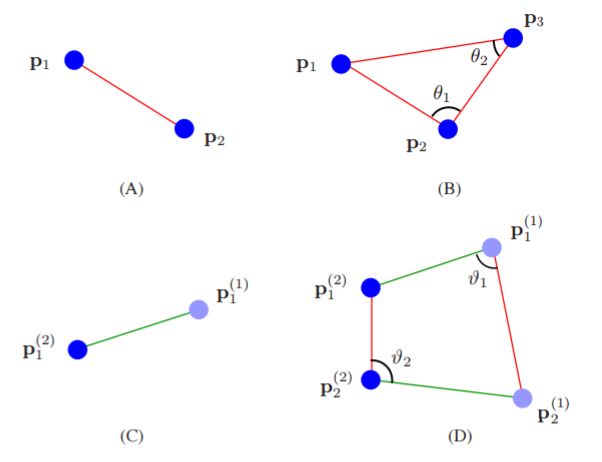
\includegraphics[width=\textwidth/2]{figure_1.png}
\caption{四种场景:(A)两个节点的空间协作(红色的连接);(B)三个节点的空间协作;(C)一个节点的时间协作(绿色的连接);(D)两个节点的时空协作。}
\end{figure}

在这些场景中,位置状态就是节点的位置,节点通过和位置已知的锚点和位置未知的邻居节点的测距中获得位置信息。
在接下来的讨论中,在时间步为n时,$\bm{K}^{(n)}_{i,i}$表示节点i从锚点获取的信息;$\bm{u}_{i,j}^{(n)}$表示节点i和j连线的单位方向向量;$\lambda^{(n)}_{i,j}=\lambda^{(n)}_{j,i}$表示节点i和j之间的测距信息强度(RII);$\bm{u}_{i,i}^{(n)}$表示链接节点i在时间步为n和n+1时的位置的单位方向向量;$\lambda^{(n)}_{i,i}$表示节点i的速度信息强度(SII)。

\textbf{场景A:}两个节点通过彼此测距协作来确定它们的位置,即位置状态是$\bm{p}_1$和$\bm{p}_2$,测距信息是$\bm{J}_r(\bm{v}_{1,2})$,其中$\bm{v}_{1,2}=\sqrt{\lambda_{1,2}}\bm{u}_{1,2}$,因此,基于(1)式我们得到这种场景的FIM是:
\begin{equation}
\bm{J}_A=\left[
\begin{array}{cc}
\bm{K}_{1,1}+\bm{J}_r(\bm{v}_{1,2})&-\bm{J}_r(\bm{v}_{1,2})\\
-\bm{J}_r(\bm{v}_{1,2})&\bm{K}_{2,2}+\bm{J}_r(\bm{v}_{1,2})\\
\end{array}
\right]
\end{equation}
%\begin{figure*}[!t]
\begin{equation*}
\bm{J}_B=\left[
\begin{array}{ccc}
\bm{K}_{1,1}+\bm{J}_r(\bm{v}_{1,2})+\bm{J}_r(\bm{v}_{1,2}) & -\bm{J}_r(\bm{v}_{1,2}) & -\bm{J}_r(\bm{v}_{1,3})\\
-\bm{J}_r(\bm{v}_{1,2}) &\bm{K}_{2,2}+\bm{J}_r(\bm{v}_{1,2})+\bm{J}_r(\bm{v}_{2,3}) & -\bm{J}_r(\bm{v}_{2,3})\\
 -\bm{J}_r(\bm{v}_{1,3}) & -\bm{J}_r(\bm{v}_{2,3})&
\bm{K}_{3,3}+\bm{J}_r(\bm{v}_{1,3})+\bm{J}_r(\bm{v}_{2,3})\\
\end{array}
\right]
\end{equation*}
%\hrulefill
%\vspace*{4pt}
%\end{figure*}

\textbf{场景B:} 三个节点通过彼此测距协作确定它们的位置,即位置状态是$\bm{p}_1,\bm{p}_2$和$\bm{p}_3$,测距信息是$\bm{J}_r(\bm{v}_{i,j})$对于$i,j\in \{1,2,3\},i\neq j$,其中$\bm{v}_{i,j}=\sqrt{\lambda_{i,j}}\bm{u}_{i,j}$,因此,基于式(1)我们可以得到这种情形的FIM由(3)给出,在下一页的最开始的地方。

\textbf{场景C:}单节点在两个不同的时刻通过速度测量协作来确定自身的位置,即位置状态是$\bm{p}^{(1)}_1$和$\bm{p}^{(2)}_1$,速度测量的信息是$\bm{J}_r(\bm{t})$,其中$\bm{t}=\sqrt{\lambda^{(1)}_{1,1}}\bm{u}_{1,1}^{(1)}$.因此基于(1),我们得到这种场景的FIM是:
\[\bm{J}_C=\left[
\begin{array}{cc}
\bm{K}_{1,1}^{(1)}+\bm{J}_r(\bm{t})&-\bm{J}_r(\bm{t})\\
-\bm{J}_r(\bm{t})&\bm{K}_{2,2}^{(2)}+\bm{J}_r(\bm{t})\\
\end{array}\right]
\]

\textbf{场景D:}两个节点在两个不同的时刻协作来确定它们的位置,即,位置状态是$\bm{p}_1^{(1)},\bm{p}_2^{(1)},\bm{p}_1^{(2)}$和$\bm{p}_2^{(2)}$,每个节点测量自身的速度和相对另一节点的距离,并且
\begin{itemize}  
\item 测距信息是$\bm{J}_r(\bm{v}_{1,2})$和$\bm{J}_r(\bm{w}_{i,j})$,其中$\bm{v}_{1,2}=\sqrt{\lambda_{1,2}^{(1)}}\bm{u}^{(2)}_{1,2}$,而$\bm{w}_{1,2}=\sqrt{\lambda_{1,2}^{(2)}}\bm{u}^{(1)}_{1,2}$
\item 测速信息是$\bm{J}_r(\bm{t}_1)$和$\bm{J}_r(\bm{t}_2)$,其中$\bm{t}_i=\sqrt{\lambda_{i,i}^{(1)}}\bm{u}^{(1)}_{i,i}$
\end{itemize}
因此,基于(1)式我们得到这种类形的FIM是
\[
\bm{J}_D=\left[
\begin{array}{cc}
\bm{J}^{(1)}_A+\bm{T}&-\bm{T}\\
-\bm{T}&\bm{J}^{(2)}_A+\bm{T}\\
\end{array}
\right]
\]
其中$\bm{J}^{(1)}_A$和$\bm{J}^{(2)}_A$由(2)式给出,上标代表了时间步长,$\bm{T}=\text{diag}\{\bm{J}_r(\bm{t}_1),\bm{J}_r(\bm{t}_2)\}$.
\section{空间信息耦合}
在这一节中,我们推导了场景A和场景B的EFIM,并且描述了场景B中由于空间协作导致的信息耦合。由于篇幅所限,这篇文章的大部分证明略去。
\begin{proposition}
场景A中节点1的EFI是
\[
\bm{J}_e=\bm{K}_{1,1}+(1-\mu_2^{1,1})\bm{J}_r(\bm{v}_{1,2})
\]
其中
\begin{eqnarray*}
\mu_2^{1,1}=&\bm{v}^T_{1,2}(\bm{K}_{2,2}+\bm{J}_r(\bm{v}_{1,2}))^{-1}\bm{v}_{1,2}\\
=&1-(1+\lambda_{1,2}\bm{u}^T_{1,2}\bm{K}^{-1}_{2,2}\bm{u}_{1,2})^{-1}.
\end{eqnarray*}
此外,$\bm{J}_e \preceq \bm{K}_{1,1}+\bm{J}_r(\bm{v}_{1,2}).$
\end{proposition}
\begin{remark}
场景A中节点1的EFIM是来自锚点和来自与节点2的协作的信息之和。协作在与节点2的连线方向上增加了信息,而节点1可以有效利用的RII随RII $\lambda_{1,2}$增大而增大而随节点2位置在$\bm{u}_{1,2}$方向的不确定性(即$\bm{u}^T\bm{K}^{-1}_{2,2}\bm{u}_{1,2}$)的增大而减小。此外,有效RII总是小于或等于RII。当锚点在节点1,2连线方向上给节点2提供无穷大的信息量时取等号,而当锚点
在这一方向上不提供任何信息时取0。
\end{remark}
\begin{proposition}
在场景B中节点1的EFIM是
\begin{equation}
\begin{split}
\bm{J}_e=\bm{K}_{1,1}+(1-\mu_2^{1,1})\bm{J}_r(\bm{v}_{1,2})+(1-\mu_3^{1,1})\bm{J}_r(\bm{v}_{1,3})\\
+\delta\bm{J}_r(\mu_2^{1,3}\bm{v}_{1,2}+\mu_3^{1,2}\bm{v}_{1,3})
\end{split}
\end{equation}
其中$\mu_i^{j,k}=\bm{v}^T_{j,i}(\bm{K}_{i,i}+\bm{J}_r(\bm{v}_{1,i}))^{-1}\bm{v}_{k,i}$,并且$\delta=(1+\mu_2^{3,3}+\mu_3^{2,2})^{-1}$.除此之外,$\bm{J}_e \preceq \bm{K}_{1,1}+\bm{J}_r(\bm{v}_{1,2})+\bm{J}_r(\bm{v}_{1,3})$.
\end{proposition}
\begin{remark}
命题2说明了场景B下节点1的EFIM是4项的和。第一项对应着从锚点获取的信息,其他三项对应着由于空间协作获得的信息。第二项和第三项对应着沿着与节点2和节点3的连线方向获取的有效信息,而最后一项代表着由于节点2和3协作造成的信息耦合。最后一项是一个秩一阵,有一个非负的特征值$\delta ||\mu_2^{1,3}\bm{v}_{1,2}+\mu_3^{1,2}\bm{v}_{1,3}||^2$并且这个特征值对应的特征向量是$\mu_2^{1,3}\bm{v}_{1,2}+\mu_3^{1,2}\bm{v}_{1,3}$,这个方向既依赖于RII,又依赖于节点2和3位置的不确定性,还和节点的空间拓扑有关。
\end{remark}
接下来我们将说明节点2和3的协作强度如何影响节点1的EFIM.
\begin{corollary}
设$\lambda_{2,3}$和$\tilde{\lambda}_{2,3}$分别表示节点2和节点3之间两个RII,并且$(\mu_2^{1,3},\mu_3^{1,2},\delta),(\tilde{\mu}_2^{1,3},\tilde{\mu}_3^{1,2},\tilde{\delta})$分别表示命题2中对应的两组参数,而其他参数均相同。那么:
\begin{equation}
\delta \bm{J}_r(\mu_2^{1,3}\bm{v}_{1,2}+\mu_3^{1,2}\bm{v}_{1,3}) \preceq \tilde{\delta} \bm{J}_r(\tilde{\mu}_2^{1,3}\bm{v}_{1,2}+\tilde{\mu}_3^{1,2}\bm{v}_{1,3})
\end{equation}
当且仅当$\lambda_{2,3}\leq \tilde{\lambda}_{2,3}$。此外
\[
\lim_{\lambda_{2,3} \rightarrow \infty}\delta \bm{J}_r(\mu_2^{1,3}\bm{v}_{1,2}+\mu_3^{1,2}\bm{v}_{1,3})=\bar{\delta} \bm{J}_r(\bar{\mu}_2^{1,3}\bm{v}_{1,2}+\bar{\mu}_3^{1,2}\bm{v}_{1,3})
\]
其中
\[
\bar{\mu}_2^{1,3}=\bm{v}_{1,2}^T(\bm{K}_{2,2}+\bm{J}_r(\bm{v}_{1,2}))^{-1}\bm{u}_{2,3}
\]
\[
\bar{\mu}_3^{1,2}=\bm{v}_{1,3}^T(\bm{K}_{3,3}+\bm{J}_r(\bm{v}_{1,3}))^{-1}\bm{u}_{2,3}
\]
\[
\bar{\delta}=(\bm{u}_{2,3}^T((\bm{K}_{2,2}+\bm{J}_r(\bm{v}_{1,2}))^{-1}+(\bm{K}_{3,3}+\bm{J}_r(\bm{v}_{1,3}))^{-1})\bm{u}_{2,3})^{-1}.
\]
\end{corollary}
\begin{remark}
从(5)中可以知道,当节点2,3方向保持不变时,节点1从和节点2和3协作中获得的信息随着节点2和3之间的RII的增大而增大。另外,这个信息量的上界是在节点2和3之间测距是理想情况时取得。
\end{remark}
在下面这个推论中,我们将说明如果从协作中获得的信息是分别和节点2,节点3的测距信息的加权和这种情形。
\begin{corollary}
场景B中节点1的EFIM可以写成
\[
\bm{J}_e=\bm{K}_{1,1}+\eta_1 \bm{J}_r(\bm{v}_{1,2})+\eta_2 \bm{J}_r(\bm{v}_{1,3}),\eta_1,\eta_2 \geq 0
\]
当且仅当至少下面至少有一个条件满足:
\begin{itemize}
\item{三个节点共线}
\item $\lambda_{1,2}\cdot \lambda_{1,3}\cdot \lambda_{2,3}=0$
\item $\bm{u}_{1,2}^T(\bm{K}_{2,2}+\bm{J}_r(\bm(v)_{1,2}))^{-1}\bm{u}_{2,3}=0$
\item $\bm{u}_{1,3}^T(\bm{K}_{3,3}+\bm{J}_r(\bm(v)_{1,3}))^{-1}\bm{u}_{2,3}=0$
\end{itemize}
\end{corollary}
接下来我们将说明如果锚点提供各向同性的信息给节点2,3,那么权重参数$\mu_i^{j,k}$可以写成$\theta_1=\angle \{\bm{u}_{1,2},\bm{u}_{2,3}\}$和$\theta_2=\angle \{\bm{u}_{1,3},\bm{u}_{2,3}\}$的函数。
\begin{corollary}
如果$\bm{K}_{i,i}=\xi_i\bm{I}$对于$i=2,3$成立,则场景B中节点1的EFIM为
\begin{equation*}
\begin{split}
\bm{J}_e=\bm{K}_{1,1}+\frac{\xi_2}{\xi_2+\lambda_{1,2}}\bm{J}_r(\bm{v}_{1,2})+\frac{\xi_3}{\xi_3+\lambda_{1,3}}\bm{J}_r(\bm{v}_{1,3})\\
+\delta\bm{J}_r(\mu_2^{1,3}\bm{v}_{1,2}+\mu_3^{1,2}\bm{v}_{1,3})
\end{split}
\end{equation*}
其中
\[
\mu_2^{1,3}=\frac{\sqrt{\lambda_{1,2}\lambda_{2,3}}\cos \theta_1}{\xi_2+\lambda_{1,2}}
\]
\[
\mu_3^{1,2}=\frac{\sqrt{\lambda_{1,3}\lambda_{2,3}}\cos \theta_2}{\xi_3+\lambda_{1,3}}
\]
\[
\mu_2^{3,3}=\frac{\lambda_{2,3}}{\xi_2}(1-\frac{\lambda_{1,2}\cos^2 (\theta_2)}{\xi_2+\lambda_{1,2}})
\]
\[
\mu_3^{2,2}=\frac{\lambda_{2,3}}{\xi_3}(1-\frac{\lambda_{1,3}\cos^2 (\theta_2)}{\xi_3+\lambda_{1,3}})
\]
\end{corollary}
\begin{remark}
这个结果说明了如果$(i)$节点2和3来自锚点或先验的信息是各向同性的$(ii)\bm{u}_{1,2}\perp\bm{u}_{2,3}$或者$\bm{u}_{1,3}\perp\bm{u}_{2,3}$,那么节点1通过写作获得的信息是分别来自节点2的测距信息的加权和。
\end{remark}
\section{空时信息耦合}
在本节中,我们推导出了场景C和D下节点1在时间步2时的EFIM,并且描述了场景D中由于空时协作产生的信息耦合。
\begin{proposition}
场景C中节点1的EFIM是
\[
\bm{J}_e=\bm{K}_{1,1}^{(2)}+\frac{\lambda_{1,1}^{(1)}}{1+\lambda_{1,1}^{(1)}\bm{u}_{1,1}^T(\bm{K}_{1,1}^{1})^{-1}\bm{u}_{1,1}}\bm{J}_r(\bm{u}_{1,1})
\]
此外$\bm{J}_e \preceq \bm{K}_{1,1}^{(2)}+\bm{J}_r(\bm{t})$.
\end{proposition}
\begin{remark}
与场景A类似,场景C中时间步为2时节点1的EFIM是从锚点获取的信息和与节点1在时间步为1时的协作信息之和。协作在节点1在两个时刻位置连线的方向上增加了信息,而节点1可以有效利用的SII随SII $\lambda_{1,1}^{(1)}$的增加而增大而随着节点1在时间步1的位置不确定性(即方向$\bm{u}_{1,1}^T(\bm{K}_{1,1}^{(1)})^{-1}\bm{u}_{1,1}$)的增大而减小。此外,有效的SII总是小于等于SII,当锚点给时间步1时的节点提供无穷大的信息时取等号,当不提供任何信息时取0.
\end{remark}
\begin{proposition}
场景D中节点1在时间步2时的EFIM是
\begin{equation}
\begin{split}
\bm{J}_e=\bm{K}_{1,1}^{(2)}+&[1-\bm{v}_{1,2}^T(\bm{K}_{2,2}^{(2)}+\bm{H}_{1,2})^{-1}\bm{v}_{1,2}]\bm{J}_r(\bm{v}_{1,2})\\
+&[1-\bm{t}_1^T(\bm{K}_{1,1}^{(1)}+\bm{H}_{1,1})^{-1}\bm{t}_1]\bm{J}_r(\bm{t}_1)\\
+&\delta \bm{J}_r(\nu_2 \bm{v}_{1,2}+\nu_1 \bm{t}_1)
\end{split}
\end{equation}
此外$\bm{J}_e \preceq \bm{K}_{1,1}^{(2)}+\bm{J}_r(\bm{v}_{1,2})+\bm{J}_r(\bm{t}_1)$
\end{proposition}
\begin{remark}
和场景B类似,命题4说明了在场景D中,时间步2时节点1的EFIM是4项的和。第一项对应着从锚点获得的信息,其余的项对应着通过协作获得的信息。第二和第三项分别是节点2在时间步2和节点1进行空间协作以及和自身在时间步1的时间协作获得的信息。而最后一项对应着耦合项。最后一项是一个秩一阵,有一个非负的特征值为$\delta||\nu_2\bm{v}_{1,2}+\nu_1\bm{t}_1||^2$,对应的特征向量为$\nu_2\bm{v}_{1,2}+\nu_1\bm{t}_1$。这个方向依赖于RII,SII,协作节点位置的不确定度以及节点在空间上的拓扑。特别的,当$\bm{t}_2^T(\bm{K}_{2,2}^{(1)})^{-1}\bm{w}_{1,2}=0$时,比如$\bm{K}_{2,2}^{(1)}=\xi_{2,2}^{(1)}\bm{I}$且$\bm{u}_{1,2}^{(1)} \perp\bm{u}_{2,2}^{(1)}$,最后一项为0.
\end{remark}
\section{数值结果}
在本节中,我们给出若干个含有信息耦合的EFIM的数值的例子。特别的,我们将考察节点的网络拓扑如何影响信息耦合项。

信息耦合项是协作节点方向加权组合作外积得到的,对于场景B,权系数是$\sqrt{\delta}\mu_2^{1,3}$和
$\sqrt{\delta}\mu_3^{1,2}$,对于场景D权系数是$\sqrt{\delta}\nu_2$和
$\sqrt{\delta}\nu_1$,图2和图3分别说明了这些系数对于角度$\theta_1=\angle \{\bm{u}_{1,2},\bm{u}_{2,3}\},\theta_2=\angle \{\bm{u}_{1,3},\bm{u}_{2,3}\}$或者$\vartheta_1=\angle \{\bm{u}_{1,1},\bm{u}_{1,2}^{(1)}\},\vartheta_2=\angle \{\bm{u}_{2,2},\bm{u}_{1,2}^{(2)}\}$的依赖关系。在数值结果里,我们设
$\bm{K}_{2,2}=\bm{K}_{3,3}=\bm{K}_{2,2}^{(2)}=\bm{K}_{2,2}^{(1)}=\bm{K}_{1,1}^{(1)}=\bm{I}$,所以的RII和SII都取1,并且$\bm{u}_{1,1}^T\bm{u}_{1,2}^{(2)}=0$.

在图2中,我们可以看到$\sqrt{\delta}\mu_2^{1,3}$和$\sqrt{\delta}\mu_3^{1,2}$,即$\bm{v}_{1,2}$或$\bm{v}_{1,3}$的权重,当$\bm{u}_{1,2}$和$\bm{u}_{1,3}$正交于$\bm{u}_{2,3}$时分别为0.此外,这两项在节点1,2,3共线时达到最大值。

类似的,在图3中,我们可以看到$\sqrt{\delta}\nu_2$和$\sqrt{\delta}\nu_1$,即耦合项中$\bm{v}_{1,2}$或$\bm{t}_1$的系数,当$\bm{u}_{2,2}$正交于$\bm{u}_{1,2}^{(2)}$且$\bm{u}_{1,1}$正交于$\bm{u}_{1,2}^{(1)}$时分别为0。此外,这两项当节点2在时间步1和2与节点1在时间步2共线或者节点1在时间步1和2与节点2在时间步1共线时为0.
%\section{结论}
%略
%\begin{thebibliography}{1}
%\item{略}
%\end{thebibliography}
%证明思路,找到一个数,对这个数求逆
%\includepdf{page5.pdf}
%\end{document}
% \documentclass[10pt,conference]{IEEEtran}
% \usepackage{xeCJK}%preamble part
% \usepackage{graphicx}
% \usepackage{indentfirst}
% \usepackage{enumerate}
% \usepackage[a4paper, inner=1.5cm, outer=3cm, top=2cm, bottom=3cm, bindingoffset=1cm]{geometry}
% \usepackage{epstopdf}
% \usepackage{listings}
% \usepackage{multicol}
% \usepackage{array}
% \usepackage{fontspec}
% \usepackage{bm}
% \usepackage{gensymb}
% \usepackage{todonotes}
% \usepackage{amsmath, amsthm, amssymb}
% \usepackage[citecolor=blue]{hyperref}
% \newtheorem{definition}{Definition}
% \newtheorem{thm}{Theorem}[section]
% \newtheorem{thm}{Theorem}
% \newtheorem{cor}{Corollary}
% \newtheorem{proposition}{Proposition}
% \newtheorem{lem}{Lemma}
% \newtheorem{remark}{Remark}
% \DeclareMathOperator{\sgn}{sgn}
% \theoremstyle{remark}
% \newtheorem*{rem}{Remark}
% \setCJKmainfont[BoldFont={SimHei}]{SimSun}
% \setCJKmonofont{SimSun}
% \setmainfont{Times New Roman}
% \newCJKfontfamily[hei]\heiti{SimHei}
% \setlength{\extrarowheight}{4pt}
% \setlength{\parindent}{1cm}
 
% \begin{document}
% \onecolumn
% \title{宽带定位的理论极限--第二部分:协作网络} 
% \author{\fontsize{12pt}{\baselineskip}{沈渊,清华大学电子工程系副教授}}
% \maketitle
% \begin{multicols}{2}
% \begin{abstract}
\title{第三篇--宽带定位的理论极限---第二部分:协作网络(节选)$^{[3]}$}
%第三篇论文的翻译,原文的题目是
%Fundamental Limits Of Wideband Localization--Part II: Cooperative Networks
%由于原文较长,翻译部分只针对原文关于EFIM的一阶上下界的部分。
%\end{abstract}


对于每个移动节点,EFIM的准确表达式非常复杂。但是我们可以找到每个节点EFIM的上下界,从而获得对定位问题的洞见。

\begin{proposition}
设$\bm{J}_e^A(\bm{p}_k)=\bm{F}(\mu_k,\eta_k,\vartheta_k)$表示节点k从锚点获得的定位信息,$\bm{C}_{kj}=\bm{F}(\nu_{kj},0,\phi_{kj})$表示该节点和节点j协作的测距信息RI。节点k的EFIM $\bm{J}_e(\bm{p}_k)$满足如下不等式:
\[
\bm{J}_e^L(\bm{p}_k) \preceq \bm{J}_e(\bm{p}_k) \preceq \bm{J}_e^U(\bm{p}_k)
\]
其中
\begin{eqnarray}
\bm{J}_e^L(\bm{p}_k)=\bm{J}_e^A(\bm{p}_k)+\sum_{j\in \mathcal{N}_a \backslash {k}} \xi_{kj}^L \bm{C}_{kj}\\
\bm{J}_e^U(\bm{p}_k)=\bm{J}_e^A(\bm{p}_k)+\sum_{j\in \mathcal{N}_a \backslash {k}} \xi_{kj}^U \bm{C}_{kj}
\end{eqnarray}
\end{proposition}
%\end{multicols}
%\hrulefill
\begin{proof}
不失一般性,我们假设k=1.

下界:考虑EFIM$\bm{J}_e^L(\bm{P})$为:
\begin{equation}
\bm{J}_e^L(\bm{P})=\left[
\begin{array}{cccc}
\bm{J}_e^A(\bm{p}_1)+\sum_{j\in \mathcal{N}_a\backslash \{1\}}\bm{C}_{1,j}&-\bm{C}_{1,2}& \dots & -\bm{C}_{1,N_a}\\
-\bm{C}_{1,2} &\bm{J}_e^A(\bm{p}_2)+\bm{C}_{1,2} & \dots & 0\\
\vdots & \vdots & \ddots & \vdots\\
-\bm{C}_{1,N_a} & 0 & \dots & \bm{J}_e^A(\bm{p}_{N_a})+\bm{C}_{1,N_a}
\end{array}
\right]
\end{equation}
%\hrulefill
%\begin{multicols}{2}
这个矩阵是令$\bm{J}_e(\bm{P})$中所有的$\bm{C}_{kj}=0$,对于$1\le k,j \leq N_a$.这个EFIM对应着节点2到$N_a$的协作完全被忽略。通过线性代数的指数可以证明$\bm{J}_e^L(\bm{P})\preceq \bm{J}_e^L(\bm{P})$,这也可直观相符,因为没有利用节点2到$N_a$的协作信息。利用EFI的方法,我们可以得到节点1的EFIM是:
\begin{equation*}
\begin{split}
&\bm{J}_e^L(\bm{p}_1)=\bm{J}_e^A(\bm{p}_1)\\
&+\sum_{j\in \mathcal{N}_a \backslash \{1\}}[\bm{C}_{1,j}-\bm{C}_{1,j}(\bm{J}_e^A(\bm{p}_j)+\bm{C}_{1,j})^{-1}\bm{C}_{1,j}]
\end{split}
\end{equation*}
因为$\bm{C}_{1,j}=\nu_{1,j}\bm{q}_{\phi_{1,j}}\bm{q}_{\phi_{1,j}}^T$,其中$\bm{q}_{\phi_{1,j}}\triangleq=[\cos(\phi_{1,j}),\sin(\phi_{1,j})]^T$,我们可以将$\bm{J}^L_e(\bm{p}_1)$表示成:
\begin{equation}
\bm{J}_e^L(\bm{p}_1)=\bm{J}_e^A(\bm{p}_1)
+\sum_{j\in \mathcal{N}_a \backslash \{1\}}\xi_{1,j}^L\bm{C}_{1,j}
\end{equation}
其中$\xi_{1,j}^L\triangleq 1-\nu_{1,j}\bm{q}^T_{\phi_{1,j}}(\bm{J}^A_e(\bm{p}_j)+\bm{C}_{1,j})^{-1}\bm{q}_{\phi_{1,j}}$.系数$\xi_{1,j}^L$可以进一步化简为
\begin{equation}
\begin{split}
\xi_{1,j}^L=&1-\nu_{1,j}\bm{q}^T_{\vartheta_j-\phi_{1,j}}\\
&\cdot (\text{diag}\{\mu_j,\eta_j\}+\nu_{1,j}\bm{q}_{\vartheta_j-\phi_{1,j}}\bm{q}^T_{\vartheta_j-\phi_{1,j}})^{-1}\bm{q}_{\vartheta_j-\phi_{1,j}}\\
=&\frac{1}{1+\nu_{1,j}\delta_j(\phi_{1,j})}
\end{split}
\end{equation}
其中
$$\delta_j(\phi_{1,j})=\frac{1}{\mu_j}\cos^2(\vartheta-\phi_{1,j})+\frac{1}{\eta_j}\sin^2(\vartheta-\phi_{1,j})$$

上界: 考虑EFIM$\bm{J}_e^U(\bm{P})$为:
%\end{multicols}
%\hrulefill
\begin{equation}
\bm{J}_e^U(\bm{P})=\left[
\begin{array}{cccc}
\bm{J}_e^A(\bm{p}_1)+&-\bm{C}_{1,2}& \dots & -\bm{C}_{1,N_a}\\
\sum_{j\in \mathcal{N}_a\backslash \{1\}}\bm{C}_{1,j}&&&\\
-\bm{C}_{1,2} &\bm{J}_e^A(\bm{p}_2)& \dots & 0\\
&+\bm{C}_{1,2}+\sum_{j\in \mathcal{N}_a\backslash \{1,2\}}2\bm{C}_{1,j} &&\\
\vdots & \vdots & \ddots & \vdots\\
-\bm{C}_{1,N_a} & 0 & \dots & \bm{J}_e^A(\bm{p}_{N_a})\\
&&&+\sum_{j\in \mathcal{N}_a\backslash \{1\}}\bm{C}_{1,j}2\bm{C}_{1,N_a}\\
\end{array}
\right]
\end{equation}
%\hrulefill
%\begin{multicols}{2}
这个矩阵可以通过把$\bm{J}_e^(\bm{P})$种对角元$\bm{C}_{kj}$扩大一倍同时让非对角元$-\bm{C}_{kj}=0$,对$1\le k,j\leq N_a$.用线性代数的知识我们可以证明$\bm{J}_e^U(\bm{P}) \succeq \bm{J}_e(\bm{P})$,这也符合直观,因为节点2到$N_a$之间有了更多的协作。利用EFI的方法,我们可以得到节点1的EFIM是:
\begin{equation*}
\bm{J}_e^U(\bm{p}_1)=\bm{J}_e^A(\bm{p}_1)
+\sum_{j\in \mathcal{N}_a \backslash \{1\}}\xi_{1,j}^U\bm{C}_{1,j}
\end{equation*}
其中
\begin{equation}
\xi_{1,j}^U =\frac{1}{1+\nu_{1,j}\tilde{\delta}_j(\phi_{1,j})}
\end{equation}
而$$\tilde{\delta}_j(\phi_{1,j})=\frac{1}{\tilde{\mu}_j}\cos^2(\tilde{\vartheta}-\phi_{1,j})+\frac{1}{\tilde{\eta}_j}\sin^2(\tilde{\vartheta}-\phi_{1,j})$$
而$\tilde{\mu}_j,\tilde{\eta}_j,\tilde{\vartheta}_j$满足:
$$
\bm{F}(\tilde{\mu}_j,\tilde{\eta}_j,\tilde{\vartheta}_j)=\bm{J}^A_e(\bm{p}_j)+\sum_{k\in \mathcal{N}_a\backslash \{1,j\}} 2\bm{C}_{jk}
$$
%\end{multicols}
\end{proof}
%\end{document}
\title{外文资料原文的索引}
\begin{translationbib}
\item S. Mazuelas, Y. Shen and M. Z. Win, "Information Coupling in Cooperative Localization," in IEEE Communications Letters, vol. 15, no. 7, pp. 737-739, July 2011.
\item S. Mazuelas, Y. Shen and M. Z. Win, "Spatio-temporal information coupling in cooperative network navigation," 2012 IEEE Global Communications Conference (GLOBECOM), Anaheim, CA, 2012, pp. 2403-2407.
\item Y. Shen, H. Wymeersch and M. Z. Win, "Fundamental Limits of Wideband Localization— Part II: Cooperative Networks" in IEEE Transactions on Information Theory, vol. 56, no. 10, pp. 4981-5000, Oct. 2010.
\end{translationbib}
\chapter{公式的推导}
\section{建模过程的一些推导过程}
\subsection{定位问题中费舍尔信息矩阵一般结构推导}\label{A_F_1}
在非协作单节点定位中,测量量的联合概率分布由式(\ref{eq:single})给出,费舍尔信息矩阵是费舍尔信息量的自然推广,在满足一定正则性的条件下,费舍尔信息矩阵可以写成:
\begin{equation}
I(\bm{p})=-\mathbb{E}_{\bm{x}}(\bigtriangledown_{\bm{p}} \log f(\vec{x}|\bm{p}))^{\textrm{T}}(\bigtriangledown_{\bm{p}} \log f(\vec{x}|\bm{p}))
\end{equation}
其中f是随机向量$\vec{x}$的密度函数,利用上面的公式,首先对式(\ref{eq:single})取对数并求梯度得:
\begin{equation}
\bigtriangledown_{\bm{p}}\ln f=-\sum_{i=1}^{N_b}\frac{||\bm{p}_i^b-\bm{p}||-x_i}{\sigma_i^2}\frac{\bm{p}^b_i-\bm{p}}{||\bm{p}^b_i-\bm{p}||}.
\end{equation}
注意到$\frac{||\bm{p}_i^b-\bm{p}||-x_i}{\sigma_i}\sim N(0,1)$,所以按照费舍尔信息矩阵的定义可得到式(\ref{eq:uu})的结果。
\section{研究成果的一些推导过程}
\subsection{两个未知节点协作最小误差界的一个充分条件}\label{B_F_0}
由式(\ref{eq:4_characteristic_polynomial}),SPEB为其所有根的倒数和,因此具有如下形式
\begin{equation}\label{eq:SPEB_GLOBAL}
\text{SPEB}=\frac{\displaystyle\sum \frac{1}{\lambda_i}+\epsilon(\frac{\cos^2(\theta)}{\lambda_1}(\sum_{i \neq 1}\frac{1}{\lambda_i})+\frac{\sin^2(\theta)}{\lambda_2}(\displaystyle\sum_{i \neq 2}\frac{1}{\lambda_i})+\frac{\cos^2(\phi)}{\lambda_3}(\sum_{i \neq 3}\frac{1}{\lambda_i})+\frac{\sin^2(\phi)}{\lambda_4}(\sum_{i \neq 4}\frac{1}{\lambda_i}))}{\displaystyle 1+\epsilon(\frac{\cos^2(\theta)}{\lambda_1}+\frac{\sin^2(\theta)}{\lambda_2}+\frac{\cos^2(\phi)}{\lambda_3}+\frac{\sin^2(\phi)}{\lambda_4})}.
\end{equation}
对固定的$\phi$,我们证明SPEB关于$\theta$是单调递减的。记$k=\frac{\cos^2 \theta}{a_1}+\frac{\sin^2 \theta}{a_2}$,$u=(\frac{1}{a_3}+\frac{1}{a_4}),v=(\frac{1}{a_1}+\frac{1}{a_2})$.~(\ref{eq:SPEB_GLOBAL})可以化为:
\begin{equation}
\text{SPEB}=u\frac{1+(\frac{1}{a_1}+\frac{1}{a_2})/u+\epsilon(\frac{1}{a_1a_2 u}+\frac{1}{a_3a_4 u}+k+(\frac{\cos^2\phi}{a_3}+\frac{\sin^2\phi}{a_4})\frac{v}{u})}{1+\epsilon(k+(\frac{\cos^2\phi}{a_3}+\frac{\sin^2\phi}{a_4}))}.
\end{equation}
SPEB可以写成关于k的反比例函数$u\frac{A+k}{B+k}$的形式,其中
\begin{align}\notag
A=&(1+(\frac{1}{a_1}+\frac{1}{a_2})/u)/\epsilon+\frac{1}{a_1a_2 u}+\frac{1}{a_3a_4 u}+(\frac{\cos^2\phi}{a_3}+\frac{\sin^2\phi}{a_4})\frac{v}{u}\\
B=&1/\epsilon+(\frac{\cos^2\phi}{a_3}+\frac{\sin^2\phi}{a_4}).
\end{align}
如果能证明$A \geq B$,那么该反比例函数关于k是单调递减的。
\begin{align}\notag
A-B=&(\frac{1}{a_1}+\frac{1}{a_2})/u\epsilon+\frac{1}{a_1a_2 u}+\frac{1}{a_3a_4 u}+(\frac{\cos^2\phi}{a_3}+\frac{\sin^2\phi}{a_4})(\frac{v}{u}-1)\\
\geq &\frac{1}{a_3a_4 u}+(\frac{\cos^2\phi}{a_3}+\frac{\sin^2\phi}{a_4})(\frac{v}{u}-1)\\
=&\frac{1}{u}((\frac{1}{a_1}+\frac{1}{a_2})(\frac{\cos^2\phi}{a_3}+\frac{\sin^2\phi}{a_4})-(\frac{\cos^2\phi}{a_3^2}+\frac{\sin^2\phi}{a_4^2})).\notag
\end{align}
由假设:$\frac{1}{a_1}+\frac{1}{a_2}\geq \max\{\frac{1}{a_4},\frac{1}{a_3}\}$,
所以$A-B\geq 0$。
\begin{equation}
k=\frac{1}{a_1}+\sin^2 \theta(\frac{1}{a_2}-\frac{1}{a_1}).
\end{equation}
根据上式,和假设条件$a_1\geq a_2$,可得在$\sin^2(\theta)\in[0,1]$的区间内k关于$\sin^2(\theta)$是单调递增的。所以由复合函数的单调性,SPEB关于$\theta$是单调递减的。
同理可证明条件$\frac{1}{a_3}+\frac{1}{a_4}\geq \max\{\frac{1}{a_1},\frac{1}{a_2}\}$是保证固定$\theta$的情况下SPEB关于$\phi \in [0,\frac{\pi}{2}]$是单调递减的。
\subsection{单节点动态定位问题等效费舍尔信息矩阵推导}\label{B_F_1}
为简化符号,记$\bm{u}:=\bm{u}_{N_a-1}$,2阶单位阵记为$\bm{I}_2$,由等效费舍尔信息矩阵的定义,有
\begin{align}\notag\label{eq:initial_efim}
  U_{N_a}=&\lambda \bm{I}_2+\bm{u}\bm{u}^{\textrm{T}}-\bm{u}\bm{u}^{\textrm{T}} U_{N_a-1}^{-1}\bm{u}\bm{u}^{\textrm{T}}\\
  =&\lambda \bm{I}_2+(1-\bm{u}^{\textrm{T}} U_{N_a-1}^{-1}\bm{u})\bm{u}\bm{u}^{\textrm{T}}.
\end{align}
因为$\bm{u}\bm{u}^{\textrm{T}}=U\begin{pmatrix}
                     1 & 0 \\
                     0 & 0
                   \end{pmatrix}U^{-1}$,其中$U$是由$\bm{u}$的方向角确定的二维旋转矩阵,所以
$U_{N_a}$相似于下面的矩阵
\begin{equation}
U_{N_a}\sim \begin{pmatrix}
                           \lambda+1-\bm{u}^{\textrm{T}} U_{N_a-1}^{-1}\bm{u} & 0 \\
                           0 & \lambda
                         \end{pmatrix}.
\end{equation}

我们定义$T_i=\lambda+1-\bm{u}^{\textrm{T}} U_{N_a-i}^{-1}\bm{u}$并设$U_{N_a-1}=\bm{u}\bm{u}^{\textrm{T}}+J_2$
由式(\ref{eq:woodbury})可得
\begin{align}\notag
T_1=&\lambda+1-\bm{u}^{\textrm{T}} (\bm{u}\bm{u}^{\textrm{T}}+J_2)^{-1}\bm{u}\\
=&\lambda+(1+\bm{u}^{\textrm{T}} J_2^{-1}\bm{u})^{-1}.
\end{align}
进一步设$v:=\bm{u}_{N_a-2}$,则$J_2=\lambda \bm{I}_2+(1-\bm{v}^{\textrm{T}} U_{N_a-2}^{-1}\bm{v})\bm{v}\bm{v}^{\textrm{T}}=V\begin{pmatrix}
                     \lambda+1-\bm{v}^{\textrm{T}} U_{N_a-2}^{-1}\bm{v} & 0 \\
                     0 & \lambda
                   \end{pmatrix}V^{-1}$
设$\bm{u}=(\cos\phi_1,\sin\phi_1)^{\textrm{T}},\bm{v}=(\cos\phi_2,\sin\phi_2)^{\textrm{T}}$,则
\begin{equation}
V^{-1}\bm{u}=\begin{pmatrix}
                     \cos\phi_2 & \sin\phi_2 \\
                     -\sin\phi_2 & \cos\phi_2
                   \end{pmatrix}\binom{\cos\phi_1}{\sin\phi_1}=\binom{\cos(\phi_1-\phi_2)}{\sin(\phi_1-\phi_2)}=:w.
\end{equation}
所以
\begin{align*}
T_1=&\lambda+(1+\bm{w}^{\textrm{T}} \begin{pmatrix}
                     \lambda+1-\bm{v}^{\textrm{T}} U_{N_a-2}^{-1}\bm{v} & 0 \\
                     0 & \lambda
                   \end{pmatrix}^{-1}\bm{w})^{-1}\\
                   =&\frac{1}{1+\cfrac{\cos^2(\phi_1-\phi_2)}{T_2}+\cfrac{\sin^2(\phi_1-\phi_2)}{\lambda}}.
\end{align*}
递推可得一般形式。
终止条件:
\begin{align*}
T_{N_a-1}&=\lambda+1-\bm{u}_1^{\textrm{T}}(\lambda\bm{I}+\bm{u}_1\bm{u}_1^{\textrm{T}})^{-1}\bm{u}_1\\
&=\lambda+\cfrac{1}{\lambda+\cfrac{1}{\lambda}}.
\end{align*}
\subsection{定理\ref{theorem:arbitrary_curve}的证明}\label{B_F_6}
式(\ref{eq:starting_or_ending})给出了式(\ref{eq:limiting_cf})右端是$\bm{p}(t)$为直线的情形。由于对于任意的平面曲线和角度序列$\{\theta_i\}$,$T_1(N_a)$是关于$N_a$的增函数且小于$\lambda+1$,因此式(\ref{eq:limiting_cf})左端的极限总是存在的。
考虑由$\bm{p}(t)$确定的角度序列$\{\theta_i\}$以如下的方式趋近于直线对应的直线序列:
\begin{equation}
\{\theta_1,\theta_2,\theta_3,\dots\}\rightarrow\{0,\theta_2,\theta_3,\dots\}\rightarrow
\{0,0,\theta_3,\dots\}\rightarrow\dots
\end{equation}
记将前n个角度置零后由式(\ref{eq:recursive_efim})确定的连分式为$K_n$,我们首先给出:
\begin{equation}\label{eq:arbitrary_curve_1}
\lim_{n\to\infty}K_n=\frac{\lambda+\sqrt{4\lambda+\lambda^2}}{2}
\end{equation}
为证式(\ref{eq:arbitrary_curve_1}),记角度序列$\{0,0,\dots,\theta_{n+1},\dots,\}$去掉前r项后对应的连分式为$K^r_n$
\begin{align}\notag
|K_n-M^*|=&\frac{|\frac{1}{M^*}-\frac{1}{K^2_n}|}{(1+\frac{1}{M^*})(1+\frac{1}{K^2_n})}\\
\leq &|\frac{1}{M^*}-\frac{1}{K^2_n}|\notag\\
= &\frac{|\frac{1}{M^*}-\frac{1}{K^3_n}|}{K^2_n(M^*+1)(1+\frac{1}{K^3_n})}\\
=& \frac{|\frac{1}{M^*}-\frac{1}{K^3_n}|}{(M^*+1)(\lambda+1+\frac{1}{K^3_n+1})}\notag\\
\leq & \frac{|\frac{1}{M^*}-\frac{1}{K^3_n}|}{(\lambda+1)^2}.\notag
\end{align}
当$r<n$ 时,
\begin{equation}
|\frac{1}{M^*}-\frac{1}{K^r_n}|\leq \frac{|\frac{1}{M^*}-\frac{1}{K^{r+1}_n}|}{(\lambda+1)^2}.
\end{equation}
因此:
\begin{equation}
|K_n-M^*|\leq \frac{|\frac{1}{M^*}-\frac{1}{K^{n}_n}|}{(\lambda+1)^{2(n-2)}}.
\end{equation}
故式(\ref{eq:arbitrary_curve_1})成立。
补充定义$K_0=\lim_{\Delta t\to 0}T_1(N_a)$这样式(\ref{eq:limiting_cf})即等价为
\begin{equation}\label{eq:equivalent_limiting_cf}
\sum_{i=1}^{\infty}(K_{i-1}-K_{i})=0.
\end{equation}
先考虑$K_0-K_1$,二者的差别是$\theta_1$是否为0,
\begin{align}\notag
K_0-K_1=&\frac{1}{1+\frac{1}{K_1^1}}-\frac{1}{1+\frac{1}{K_1^1}+\sin^2\theta_1(\frac{1}{\lambda}-\frac{1}{K_1^1})}\\
\leq & (\frac{1}{\lambda}-\frac{1}{K_1^1})\sin^2\theta_1.
\end{align}
类似式(\ref{eq:arbitrary_curve_1})的推导:
\begin{equation}
K_r-K_{r+1}\leq \sin^2\theta_{r+1}(\frac{1}{\lambda}-\frac{1}{K_{r+1}^{r+1}})\frac{1}{(\lambda+1)^{2r}}.
\end{equation}
由条件$\bm{p}'(t)$存在且连续可得切向量是连续变化的,由微分中值定理在闭区间内存在常数c使得角度变化量$\theta_i\leq c\Delta t$。
由正弦函数的单调性推出:
\begin{equation}
K_r-K_{r+1}\leq \sin^2 (c\Delta t) \frac{1}{\lambda}\frac{1}{(\lambda+1)^{2r}}.
\end{equation}
因此
\begin{equation}\label{eq:quatratic_convergence}
0\leq \sum_{i=1}^{N_a}(K_{i-1}-K_{i})\leq \sin^2 (c\Delta t) \frac{1}{\lambda}\sum_{i=1}^{\infty}\frac{1}{(\lambda+1)^{2i}}.
\end{equation}
无穷级数$\sum_{i=1}^{\infty}\frac{1}{(\lambda+1)^{2i}}$收敛,所以当$\Delta t\to 0$时$N_a\to \infty$,式(\ref{eq:equivalent_limiting_cf})成立。

%\subsection{单节点动态定位问题等效费舍尔信息衰减上下界}\label{B_F_2}
%为记号简便记$T'_1=T_1(N_a+1),T_1=T_1(N_a)$
%由于我们在连分式的第一层嵌入了新的节点,设引入的角度参数为$\theta$,于是可以得到:
%\begin{equation}
%T'_1=\lambda+\frac{1}{1+\frac{\sin^2\theta}{\lambda}+\frac{\cos^2\theta}{T_1}}.
%\end{equation}
%对固定的$T_1>\lambda$,$T'_1$是关于$\theta$的减函数,于是我们有:
%\begin{equation}
%T'_1\leq \lambda+\frac{1}{1+\frac{1}{T_1}}.
%\end{equation}
%递推下去我们可以得到结论$T_1$当各个角度的正弦值均为0时取得最大值:
%\begin{align}\label{eq:MMM}
%T_1\leq &[\lambda,1,\underbrace{\lambda,1}_{\text{repeat $N_a-1$ times}},\lambda]:=M_{N_a}\\
%\leq  & M^* \text{参见式}(\ref{eq:starting_or_ending})\notag
%\end{align}
%下面考虑$T'_1-T_1$:
%\begin{equation}
%T'_1-T_1\leq \lambda-\frac{T_1^2}{T_1+1}
%\end{equation}
%且上式右端关于$T_1$是减函数,故由式(\ref{eq:MMM})可得:
%\begin{equation}
%T'_1-T_1\leq \lambda-\frac{T_1^2}{M_{N_a}+1}
%\end{equation}

%考虑在原有基础上增加一层节点,
%于是协作层数由原来的$N_a-1$变为$N_a$。等效费舍尔信息矩阵较大的特征值分别记为$T_1,T'_1$,

%上界:
\subsection{单节点动态定位问题等效费舍尔信息衰减上下界}\label{B_F_2}
为记号简便记$T'_1=T_1(N_a+1),T_1=T_1(N_a)$
%考虑在原有基础上增加一层节点,
%于是协作层数由原来的$N_a-1$变为$N_a$。等效费舍尔信息矩阵较大的特征值分别记为$T_1,T'_1$,
为便于比较,我们在$T_1$中引入虚拟节点将其层数也拓展为$N_a$,它只有锚点的定位信息,这样它们的区别是连分式的末端$T_{N_a}=\lambda$,$T'_{N_a}=\lambda+\frac{1}{1+1/\lambda}$
对$|T_1-T'_1|$从外向里通分得:
\begin{align}\notag
|T_1-T'_1|=&\frac{|\frac{1}{T_2}-\frac{1}{T'_2}|\cos^2\theta_1}{(1+\frac{\sin^2\theta_1}{\lambda}+\frac{\cos^2\theta_1}{T_2})
(1+\frac{\sin^2\theta_1}{\lambda}+\frac{\cos^2\theta_1}{T'_2})}\\
\leq &|\frac{1}{T_2}-\frac{1}{T'_2}|.
\end{align}
继续放缩$|\frac{1}{T_2}-\frac{1}{T'_2}|$有:
\begin{align}\notag
|\frac{1}{T_2}-\frac{1}{T'_2}|= & \frac{|\frac{1}{T_3}-\frac{1}{T'_3}|\cos^2\theta_2}{(1+\lambda(1+\frac{\sin^2\theta_2}{\lambda}+\frac{\cos^2\theta_2}{T_3}))
(1+\lambda(1+\frac{\sin^2\theta_2}{\lambda}+\frac{\cos^2\theta_2}{T'_3}))}\\
\leq & |\frac{1}{T_3}-\frac{1}{T'_3}|\frac{1}{(1+\lambda)^2}.
\end{align}
逐次递推得
\begin{equation}
|T_1-T'_1|\leq \frac{1}{(1+\lambda)^{2(N_a-2)}} |\frac{1}{T_{N_a}}-\frac{1}{T'_{N_a}}|.
\end{equation}
而:
\begin{equation}
|\frac{1}{T_{N_a}}-\frac{1}{T'_{N_a}}|=\frac{1}{\lambda^2+2\lambda}.
\end{equation}
对于下界,因为$T_2,T'_2\geq \lambda$
\begin{equation}
|T_1-T'_1|\geq \frac{\cos^2\Delta\theta|\frac{1}{T_2}-\frac{1}{T'_2}|}{(1+1/\lambda)^2}.
\end{equation}
\begin{equation}
|\frac{1}{T_2}-\frac{1}{T'_2}|\geq \frac{\cos^2\Delta\theta|\frac{1}{T_3}-\frac{1}{T'_3}|}{(2+\lambda)^2}
\end{equation}
逐次递推得下界。
%\subsection{推论\ref{corollary:exponential_decreasing}的证明}\label{B_F_5}
%由定理\ref{theorem:exponential_decreasing}的结论:
%\begin{equation}
%T_{N_a}=\sum_{k=1}^{N_a-1}\Delta_{+}T_k
%\end{equation}
%因此当$N_a\geq 2$时
%\begin{equation}
%|T_{N_a}-T_{\infty}|=\sum_{k=N_a}^{\infty}\Delta_{+}T_k\leq %\frac{1}{\lambda^2+2\lambda}\sum_{k=N_a}^{\infty}\frac{1}{(\lambda+1)^{2(k-2)}}=\frac{1}{(\lambda^2+2\lambda)^2}\frac{1}{(\lambda+1)^{2(N_a-3)}}
%\end{equation}
%取$q=(\lambda+1)^2$,其余常数为C即可。
\subsection{单节点非均一测距误差等效费舍尔信息矩阵推导}\label{B_F_3}
类似式(\ref{eq:initial_efim})有:
\begin{equation}
U_{N_a}=\bm{I}+(\lambda_1-\lambda_1^2 \bm{u}^{\textrm{T}} U_{N_a-1}^{-1}\bm{u})\bm{u}\bm{u}^{\textrm{T}}.
\end{equation}
而
\begin{equation}
T_1=1+\lambda_1-\lambda_1^2 \bm{u}^{\textrm{T}} U_{N_a-1}^{-1}\bm{u}=1+(\lambda_1^{-1}+\bm{u}^{\textrm{T}}\bm{J}_2^{-1}\bm{u})^{-1}.
\end{equation}
对$J_2=\bm{I}_2+(\lambda_2-\lambda_2^2\bm{v}^{\textrm{T}} U_{N_a-2}^{-1}\bm{v})\bm{v}\bm{v}^{\textrm{T}}$提取关于$\bm{v}$的旋转矩阵即得到
式(\ref{eq:recursive_efim_second})。
另外从式(\ref{eq:recursive_efim_second})出发,设$\theta'_1\leq \theta_1$,作差:
\begin{equation}
T_1(\theta'_1)-T_1(\theta_1)=\frac{1}{A}(\cos^2\theta'_1-\cos^2\theta_1)(1-\frac{1}{T_2})\geq 0
\end{equation}
其中$A>0$,由上式可看出角度$\theta_1$越小$T_1$越大,同理$\theta_i$越小$T_i$越大,而由连分式的表达式可以看出$T_1$关于$T_2$递增,而连分式本身具有自相似性,因此诸$\theta_i$减小可以增大信息量$T_1$。

\subsection{引理~\ref{lemma:hexagon}的推导}\label{B_F_4}
  设式(\ref{eq:equiv})左边为B,$A=\lambda+\frac{3}{2}$,那么由Woodbury矩阵求逆公式有
  \begin{equation}
  (A+\frac{1}{\lambda+3/2-\frac{3/2}{\lambda+3/2}})^{-1}=A^{-1}-A^{-1}BA^{-1}.
  \end{equation}
  整理得:
  \begin{equation}
  B=A-\frac{A^2}{A+\frac{1}{\lambda+3/2-\frac{3/2}{\lambda+3/2}}}.
  \end{equation}
  通分化简得证。
\section{本文中用到的关于连分式的结论}\label{C_F}
\begin{definition}
  有限序列$t_1,t_2,\dots,t_r$满足$t_j\geq 1$对于$j\geq2$可以递推地定义有限连分式
  \begin{equation}
  [t_1,t_2,\dots,t_r]:=t_1+\frac{1} {[t_2,\dots,t_r]}.
  \end{equation}
\end{definition}
\begin{theorem}\label{thm:basic}
  设$p_j=t_j p_{j-1}+p_{j-2},q_j=t_j q_{j-1}+q_{j-2}$,$M_j=\left(\begin{matrix}p_j&p_{j-1}\\q_j&q_{j-1}\end{matrix}\right)$,
  $p_0,p_1,q_0,q_1$由$M_0=I_2$给出,且$T_j=\left(\begin{matrix}t_j&1\\1&0\end{matrix}\right)$则有下面三个恒等式:
  \begin{enumerate}
    \item $M_j=M_{j-1}T_j$,
    \item $\binom{p_j}{q_j}=(\prod_{i=1}^r T_i )\binom{1}{0}$,
    \item $[t_1,t_2,\dots,t_r]=\frac{p_r}{q_r}$.
  \end{enumerate}
\end{theorem}
\begin{theorem}\label{theorem:quadratic_cyclic}
若$\lim_{r\to \infty}[t_1,t_2,\dots,t_r]$存在,该极限是形如$\frac{a+b\sqrt{m}}{c}$的二次根式当且仅当序列$t_i$从某项开始是周期的,即$\exists c\text{和}r,\,s.t.\, t_{i}=t_{i+r},\forall i\geq c$。
\end{theorem}
\begin{remark}

对于定理\ref{theorem:quadratic_cyclic},$\lim_{r\to \infty}[t_1,t_2,\dots,t_r]$值可用二次方程不动点的方法求出\cite{ContinuedFraction}。
%设$\left(\begin{matrix}a&b\\c&d\end{matrix}\right)=(\prod_{i=1}^{rc} %T_{i+c})$,称$\left(\begin{matrix}a&b\\c&d\end{matrix}\right)$对应着分式线性变换K,如果$K(z)=\frac{az+b}{cz+d}$。
%可以证明系数为实数的分式线性变换以函数复合作为群运算与行列式为1的2阶方阵以矩阵乘积作为群运算是同构的。
%c之前的$t_i$对应着矩阵$T_i$的乘积矩阵看作分式线性变换F。可以进一步说明二次根式和T和F的有如下的关系:
%\begin{enumerate}
%  \item 首先求解$K$的不动点即解二次方程$x=\frac{ax+b}{cx+d}$得x
%  \item $F(x)=\lim_{r\to \infty}[t_1,t_2,\dots,t_r]$,F(x)即为极限$\lim_{r\to \infty}[t_1,t_2,\dots,t_r]$
%\end{enumerate}
%一般二次方程有两个根,而有限连分式的极限值是唯一的,这时可根据极限值介于序列的前两个数之间剔除一个不合理的不动点。
\end{remark}

\end{appendix}


%% 本科生进行格式审查是需要下面这个表格,答辩可能不需要。选择性留下。
% 综合论文训练记录表
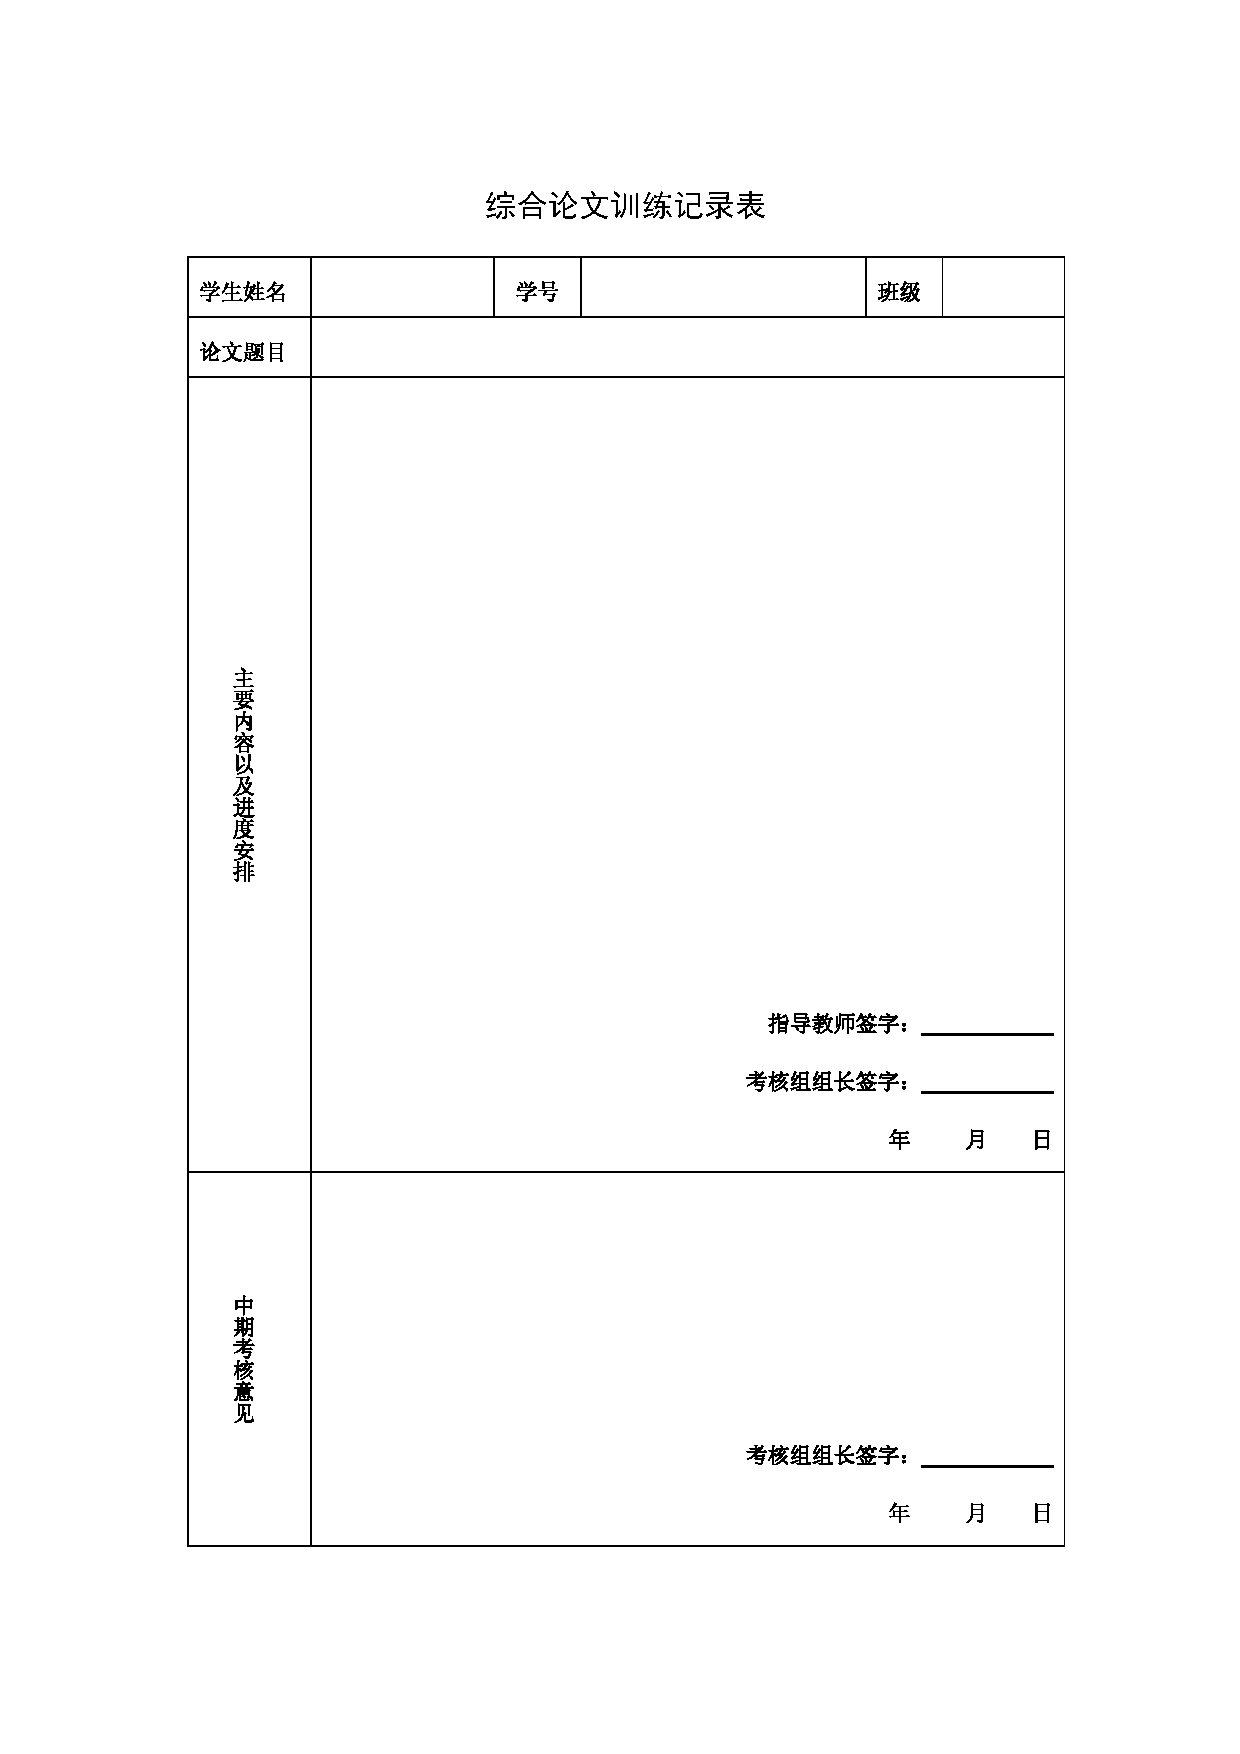
\includepdf[pages=-]{scan-record.pdf}
\end{document}
